%!TEX program = xelatex 
\documentclass[UTF8]{ctexbook}
\usepackage{clcxsj}

\makeindex

\begin{document}

\pagenumbering{Alph}
%!TEX root = ../clcxsj.tex

%%
% 对课程进行介绍
%%

\pdfbookmark{标题页}{title}
\thispagestyle{empty}

\vspace*{\stretch{1}}
\noindent\begin{minipage}{\textwidth}
\raggedleft
{\huge \bfseries 测量程序设计}
\noindent\rule[-1ex]{\textwidth}{5pt}\\[2.5ex]
\hfill\emph{\Large  C\#--WPF }
\end{minipage}

\vspace{\stretch{1}}
\noindent\rlap{%
  \begin{minipage}{\textwidth}
  \linespread{1.67}\selectfont\raggedleft
   {\bfseries  朱学军  编著}  \\
  {\bfseries  xazhuxj@qq.com }  \\
  {\bfseries 西安科技大学 }    \\
  {\bfseries  测绘科学与技术学院 }   \\
  {\bfseries } \zhdigits*{\the\year}年\zhnumber{\the\month}月
  \end{minipage}%
}

\vspace{\stretch{2}}

\newpage\thispagestyle{empty}
\begin{quote}\footnotesize
    本文档仅适用于西安科技大学测绘相关专业本科二年级以上学生教学使用。

    也可用于其他专业人员参考。

    内部文档,版权所有 \copyright{}  2018,朱学军。

    未经作者本人授权,严谨出版发行!
\end{quote}

\frontmatter
%!TEX root = ../clcxsj.tex

%%
% 对课程进行介绍
%%

\chapter{教学计划及课程目标}

\section*{教学计划}

\subsection*{教学课时}
该课程标准学时为32+8学时。总学时为48学时,上课16次32学时,上机4次8学时。

必修课,考试。笔试(50\%)+上机实验与作业(50\%)

\subsection*{学习内容}

学习面向对象的程序设计与编写;

学习基本的测量算法程序编写,学习软件界面的编写。

\section*{编程语言的选择}

注意:该课程不是再次学习某种编程语言,而是运用某种编程语言进行
测量数据处理及测量算法的编写。

可能大家只学习了C语言,C语言是面向过程的功能强大的语言,执行效率高,但界面程序编写较复杂。
现代编程语言更多的是面向对象的编程语言,高效而且兼容C语言的是 \cpp ,但界面的编写仍较复杂。
因此我们选择更加现代化的编程语言 \cs ,它语法优美,界面编写方式有 WinForm 与 WPF方式,虽然
执行效率没有 \cpp 高,但在Windows7、Windows8/8.1、Windows10+中都几乎预装了运行库 .Net Framework,
并且得到了Microsoft的大力推广,Microsoft的许多软件都在使用 \cs 开发,学习与开发成本相比与 \cpp 显著减少,
开发效率显著提升。

\cs 的语法与JAVA的许多语法是极其相似的,现代软件工程的许多方法也可以用 \cs 去实现。因此,在本课程中我们将
学习 \cs 编程语言,并且会学习如何运用 \cs 语言进行测量程序设计及测量数据处理。

现代软件基本上都具有简洁易用的界面,我们还将学习WPF的界面编写技术,为我们的程序设计处美观简洁的界面,
这些都包含在 \cs 之中。

\section*{编程环境与工具}

由于.Net Framwork 正在向 .Net Core发展,而在即将发布的.Net 6、Net 8 中,以.Net Core为基础将.Net 的各种技术整合。
而且 \cs 已经更新到8.0、9.0、10.0,且11也在预览之中。为了探究新的技术,
本课程的基本编程工具定为Visual Studio,版本理论上为2017及更新版,推荐大家用Visual Studio 2019或2022社区版(Community)。

\section*{参考教材}

\cs 语言及WPF界面编写参考马骏主编,人民邮电出版社出版,《\cs 程序设计及应用教程》第3版。

测量算法参考本教程(一直更新中......)。
 %%课程介绍及课程目标

\tableofcontents

\mainmatter
\include{chapter/csenv/csenv}            %%C#开发环境 与 从C走向C\#
%!TEX root = ../../clcxsj.tex

\chapter{ \cs 语言基础}

\cs 程序设计语言是类 C 语言,基本语法与 C 基本相同, 本章主要讲解 \cs 中不同于 C 的基础语法。

\section{ \cs 中的数据类型}
 为保持 \cs 语言的高效性,\cs 中的数据类型分为两类:值类型 (value type) 和引用类型 (reference type)。
值类型的变量直接包含它们的数据,也就是直接在栈中保存变量的值, 变量的值自动生成、自动释放;
而引用类型的变量存储对数据的引用,即在堆中生成变量的值,在栈中保存堆中值的地址,在堆中生成的变量不自动释放,靠 .Net 架构回收。

\subsection{值类型}
 \cs  的值类型进一步划分为简单类型 ( simple type )、枚举 ( enum )、结构( struct )
和可以为 null 的值类型 (nullable type)。

对于值类型,每个变量都有它们自己的数据副本(除 ref 和 out 参数变量外),
因此对一个变量的操作不可能影响另一个变量。

\begin{tabular}{|l|l|}
\hline
类别   & 说明 \\
\hline
简单类型   & 有符号整型:sbyte 、short 、int 、long \\
          & 无符号整型:byte、ushort、uint、ulong \\
          & Unicode 字符:char \\
          & IEEE 浮点:float、double \\
          & 高精度小数型:decimal \\
          & 布尔:bool \\
\hline
结构                & struct S {...} 形式的用户定义的类型 \\
枚举                & enum E {...} 形式的用户定义的类型   \\
可以为 null 的值类型 & 其他所有具有 null 值的值类型的扩展   \\
\hline
\end{tabular}


\subsection{引用类型}
 \cs  的引用类型进一步划分为类 (class)、接口(interface)、
数组 (array) 和委托(delegate)。
对于引用类型,两个变量可能引用同一个对象,因此对一个变量的操作可能影响另一个变量所引用的对象。

\begin{tabular}{|l|l|}
\hline
类别          & 说明 \\
\hline
类class       &  所有其他类型的最终基类:object \\
              &  Unicode 字符串:string \\
              &  class C {...} 形式的用户定义的类型 \\
\hline
接口interface     & interface I {...} 形式的用户定义的类型  \\
数组              & 一维和多维数组,例如 int[] 和 int[,]  \\
委托 delegate     & delegate int D(...) 形式的用户定义的类型  \\
\hline
\end{tabular}

 \cs 中的 string不是值类型数据,而是引用类型数据。

\subsection{自定义类型}
 \cs  程序使用类型声明 (type declaration) 创建新类型。类型声明指定新类型的名称和成员。
在  \cs  类型分类中,有五类是用户可定义的:类(class)、结构(struct)、
接口(interface)、枚举(enum) 和委托(delegate)。

注:\cs 7.0 提供了元组(tuple), \cs 9.0 提供了记录(record)。


类是定义了一个包含数据成员(字段)和函数成员(方法、属性等)的数据结构,类支持单一继承和多态。

结构与类相似,表示一个带有数据成员和函数成员的结构。
但是,与类不同,结构是值类型,不需要堆分配。
结构类型不支持用户指定的继承,所有结构类型都隐式地从类 System.Object 继承。

接口定义了一个协定,是一个公共函数成员的命名集。
实现某个接口的类或结构必须提供该接口的函数成员的实现。
一个接口可以从多个接口继承,而一个类或结构可以实现多个接口。

委托表示对具有特定参数列表和返回类型的方法的引用。
通过委托,我们能够将方法作为实体赋值给变量和作为参数传递。
委托类似于在其他某些语言中的函数指针的概念,但是与函数指针不同,委托是面向对象的,并且是类型安全的。

类、结构、接口和委托都支持泛型,因此可以通过其他类型将其参数化。

枚举是具有命名常量的独特的类型。每种枚举类型都具有一个基础类型,
该基础类型必须是八种整型之一。枚举类型的值集和它的基础类型的值集相同。

 \cs  支持由任何类型组成的一维和多维数组。与以上列出的类型不同,数组类型不必声明就可以使用。
实际上,数组类型是通过在某个类型名后加一对方括号来构造的。
例如,int[] 是一维 int 数组,int[,] 是二维 int 数组,int[][] 是一维 int 数组的一维数组。

可以为 null 的类型也不必声明就可以使用。对于每个不可以为 null 的值类型 T,
都有一个相应的可以为 null 的类型 T?,该类型可以容纳附加值 null。
例如,int? 类型可以容纳任何 32 位整数或 null 值。

\subsection{装箱与拆箱}
 \cs  的类型系统是统一的,因此任何类型的值都可以按对象处理。 \cs  中的每个类型直接或间接地从 object 类类型派生,
而 object 是所有类型的根基类。引用类型的值都被视为 object 类型,被简单地当作对象来处理。
值类型的值则通过对其执行装箱和拆箱操作按对象处理。下面的示例将 int 值转换为 object,然后又转换回 int。

\begin{lstlisting}
using System;
class Test
{
    static void Main()
    {
        int i = 123;
        object o = i;      // Boxing
        int j = (int)o;    // Unboxing
    }
}
\end{lstlisting}

当将值类型的值转换为类 object 时,将分配一个对象实例(也称为“箱子”)以包含该值,
并将值复制到该箱子中。反过来,当将一个 object 引用强制转换为值类型时,
将检查所引用的对象是否含有正确的值类型,如果有,则将箱子中的值复制出来。


\subsection{延伸阅读值类型}

实际上值类型和引用类型都是从System.Object继承的,System.Object类是 \cs 中所有类的基类。
所有值类型都隐式继承自类 System.ValueType,而类System.ValueType又继承自类 System.Object(别名object),
System.ValueType 用更合适的值类型实现重写了Object 中的虚方法。 

但任何类型都不能直接从值类型System.ValueType派生。

这样就有一个问题,值类型与引用类型都是从System.Object继承的,怎么object类型与int类型就不一样呢?

这里大致可以这样理解,.Net是动态加载运行 \cs 代码的,CLR在运行时把值类型装载到栈,把引用类型装载到堆,
栈中只提供一个引用指向堆,即引用。

\subsection{\cs 新版本中的类型}

\begin{itemize}
    \item 元组(tuple)
    
    用于将多个数据元素分组成一个轻型数据结构。
    如:
\begin{lstlisting}
(double, int) t1 = (4.5, 3);
Console.WriteLine($"Tuple with elements {t1.Item1} and {t1.Item2}.");
// Output:
// Tuple with elements 4.5 and 3.
(double Sum, int Count) t2 = (4.5, 3);
Console.WriteLine($"Sum of {t2.Count} elements is {t2.Sum}.");
// Output:
// Sum of 3 elements is 4.5.
\end{lstlisting}

    元组类型是值类型,元组元素是公共字段。元组字段的默认名称为 Item1、Item2、Item3 等。

    \item 记录(record)
    
    record类型是一种用record关键字声明的新的引用类型,与类不同的是,
    它是基于值相等而不是唯一的标识符——对象引用。
    它有着引用类型的支持大对象、继承、多态等特性,也有着结构的基于值相等的特性。
    可以说有着class和struct两者的优势,在一些情况下可以用以替代class和struct。

    如以下代码就定义了一个类Point:
\begin{lstlisting}
public record Point(string Name, double X, double Y, double Z);
\end{lstlisting}

\end{itemize}


\subsection{变量的定义}

\cs 中变量是前置定义的,需先指定类型,然后是变量名,最后是其值。
如: int i = 0;

变量可以显示指定类型,也可以隐式定义,让编译器根据变量的值进行推定,如:
var i = 0;

值类型数据可以在声明时赋初始值,引用类型变量在定义时需用new生成实例对象或
将其它实例对象的引用赋值给它,或直接赋值为null。


\section{表达式与语句}

\subsection{表达式}
表达式由操作数 (operand) 和运算符 (operator) 构成。表达式的运算符指示对操作数适用什么样的运算。
运算符的示例包括+、-、*、/ 和 new。操作数的示例包括文本、字段、局部变量和表达式。

\begin{tabular}{|l|l|}
\hline
类别            & 说明 \\
\hline
x.m            &          成员访问  \\
x(...)         &           方法和委托调用  \\
x[...]         &           数组和索引器访问  \\
x++            &        后增量  \\
x--            &           后减量  \\
new T(...)     &       对象和委托创建  \\
new T(...){...}&      使用初始值设定项创建对象  \\
new {...}      &         匿名对象初始值设定项  \\
new T[...]     &        数组创建  \\
typeof(T)      &      获取 T 的 System.Type 对象  \\
checked(x)     &    在 checked 上下文中计算表达式  \\
unchecked(x)   & 在 unchecked 上下文中计算表达式  \\
default(T)     &       获取类型 T 的默认值  \\
delegate {...} &      匿名函数(匿名方法)  \\
(T)x           &             将 x 显式转换为类型 T  \\
await x        &         异步等待 x 完成  \\
x is T         &            如果 x 为 T,则返回 true,否则返回 false  \\
x as T         &           返回转换为类型 T 的 x,如果 x 不是 T 则返回 null  \\
(T x) => y     &       匿名函数(lambda 表达式)  \\
\hline
\end{tabular}

其它的与 C 或 \cpp 语言基本相同。


\subsection{ 语句 }
程序的操作是使用语句 (statement) 来表示与实现的。

\cs 中常见的语句有:
\begin{itemize}
\item 声明语句 (declaration statement) 

    用于声明局部变量和常量。

\item 表达式语句 (expression statement) 

    用于对表达式求值。

    可用作语句的表达式包括方法调用、使用 new 运算符的对象分配、
使用 = 和复合赋值运算符的赋值、使用 ++ 和 -- 运算符的增量和减量运算以及 await 表达式。

\item 选择语句 (selection statement) 

用于根据表达式的值从若干个给定的语句中选择一个来执行。
这一组中有 if else、 switch case、 ? : 、 ??语句。

??表示如果左值为null,则用右值进行计算,如下代码所示:
\begin{lstlisting}
int? a = null;
int b = a ?? -1;
Console.WriteLine(b);  // output: -1
\end{lstlisting}

\item 迭代语句 (iteration statement) 

用于重复执行嵌入语句,常用语句有 while、do、for 和 foreach 语句。

\cs 中常用foreach语句进行循环,示例代码如下:

\begin{lstlisting}
static void Main(string[] args)
{
    foreach (string s in args)
    {
        Console.WriteLine(s);
    }
}
\end{lstlisting}


\item 跳转语句 (jump statement) 

用于转移控制,常用语句有 break、continue、goto、throw、return 和 yield 语句。

\item 异常捕捉

try...catch 语句用于捕获在块的执行期间发生的异常,try...finally 语句用于指定终止代码,不管是否发生异常,该代码都始终要执行。
    
\begin{lstlisting}
static double Divide(double x, double y)
{
    if (y == 0) throw new DivideByZeroException();
    return x / y;
}

static void Main(string[] args)
{
    try
    {
        if (args.Length != 2)
        {
            throw new Exception("Two numbers required");
        }
        double x = double.Parse(args[0]);
        double y = double.Parse(args[1]);
        Console.WriteLine(Divide(x, y));
    }
    catch (Exception e)
    {
        Console.WriteLine(e.Message);
    }
    finally
    {
        Console.WriteLine(“Good bye!”);
    }
}
\end{lstlisting}

\item checked 语句和 unchecked 语句

用于控制整型算术运算和转换的溢出检查上下文。

\begin{lstlisting}
static void Main()
{
    int i = int.MaxValue;
    checked 
    {
        Console.WriteLine(i + 1);       // Exception
    }
    unchecked
    {
        Console.WriteLine(i + 1);       // Overflow
    }
}
\end{lstlisting}

\item lock 语句

用于获取某个给定对象的互斥锁,执行一个语句,然后释放该锁。

\begin{lstlisting}
class Account
{
    decimal balance;
    public void Withdraw(decimal amount)
    {
        lock (this)
        {
            if (amount > balance)
            {
                throw new Exception("Insufficient funds");
            }
            balance -= amount;
        }
    }
}
\end{lstlisting}

\item using 语句

用于获得一个资源,执行一个语句,然后释放该资源。

\begin{lstlisting}
static void Main()
{
    using (TextWriter w = File.CreateText("test.txt"))
    {
        w.WriteLine("Line one");
        w.WriteLine("Line two");
        w.WriteLine("Line three");
    }
}
\end{lstlisting}


\end{itemize}


\section{ \cs 特殊语法}

\subsection{泛型}
在定义类时,在类名后用尖括号括起来的类型参数列表,称之为泛型。如:
\begin{lstlisting}
public class Pair<T1, T2>
{
    public T1 first;
    public T2 second;
}
\end{lstlisting}
代码中的T1与T2为类型参数。

泛型是现代编程语言非常重要的语法。

\subsection{集合}
数组Array、列表List、词典Dictionary、栈Stack、队列Queue 
是程序设计中常用的数据结构,在 \cs 中均以类库形式提供,
在\cs 程序设计中可以直接使用。

在使用这些集合类时,应尽量使用泛型集合,如动态数组:List<int>

\subsection{委托}
委托类似于C、\cpp 中的函数指针。语法为:

访问修饰符 delegate 返回类型 委托名(参数序列);

从语法上可以看出,delegate之后实际上就是函数的定义。

.Net中预定义了Func和Action委托。

Func委托代表有返回值的委托,参数最多有16个,最后一个参数必须是返回参数TResult,语法形式为:

public delegate TResult Func<in T1, ..., in T15, out TResult>(T1 arg1, ..., T15 arg15);

Action委托代表无有返回值的委托,参数最多有16个,语法形式为:

public delegate void Action<in T1,...,in T16>(T1 arg1, ..., T16 arg2);

\subsection{Lambda语句}
Lambda表达式主要用于简化委托的编写形式,是一种可用于创建委托或表达式树类型的匿名函数。语法为:

(输入参数列表) => \{表达式或语句块\}

Lambda表达式实质是一个匿名函数,如下代码所示:
\begin{lstlisting}
List<int> list = new List<int>(){1,2,3,4,5,6,7,8,10,11,12,13,14,15};
var q = list.Were( x => x%2 == 0);
\end{lstlisting}
list.Where函数中调用的就是Lambda表达式。

\subsection{迭代器}

迭代器用于逐步迭代集合(如列表和数组)。

迭代器方法或 get 访问器可对集合执行自定义迭代。 迭代器方法使用 yield return 语句返回元素,每次返回一个。 到达 yield return 语句时,会记住当前在代码中的位置。 下次调用迭代器函数时,将从该位置重新开始执行。

通过 foreach 语句或 LINQ 查询从客户端代码中使用迭代器。

如下所示代码,将输出 3 5 8

\begin{lstlisting}
using System;

namespace ConsoleApp1
{
    class Program
    {
        static void Main(string[] args)
        {
            foreach (int number in SomeNumbers())
            {
                Console.Write(number.ToString() + " ");
            }
            // Output: 3 5 8
            Console.ReadKey();

        }

        public static System.Collections.IEnumerable SomeNumbers()
        {
            yield return 3;
            yield return 5;
            yield return 8;
        }
    }
}
\end{lstlisting}

迭代器方法或 get 访问器的返回类型可以是 IEnumerable、IEnumerable<T>、IEnumerator 或 IEnumerator<T>。

可以使用 yield break 语句来终止迭代。

yield语句

\begin{lstlisting}
static IEnumerable<int> Range(int from, int to) {
    for (int i = from; i < to; i++) {
        yield return i;
    }
    yield break;
}
static void Main()
{
    foreach (int x in Range(-10,10)) {
        Console.WriteLine(x);
    }
}
\end{lstlisting}



\section{小结}
这一章我们学习了 \cs 基本语法:数据与语句,数据分为数值类型与引用类型,
数据定义时可以使用var关键字让编译器推断变量的数据类型,还可以使用泛型。

\cs 语句相对于C、\cpp 而言,出现了一些新的如lambda语句、迭代器等,
这些是许多现代语言中必不可少的语言特征,
我们将在后续课程中将其继续学习与应用。

\section{上机实验}
\begin{enumerate}
\item 冒泡排序 (Bubble Sort)

冒泡排序是一种较简单的排序算法。它重复地走访过要排序的元素列,
依次比较两个相邻的元素,如果顺序错误就把他们交换过来。
走访元素的工作是重复地进行直到没有相邻元素需要交换,也就是说该元素列已经排序完成。
这个算法的名字由来是因为越小的元素会经由交换慢慢“浮”到数列的顶端(升序或降序排列),
就如同碳酸饮料中二氧化碳的气泡最终会上浮到顶端一样,故名“冒泡排序”。

原理如下:

比较相邻的元素。如果第一个比第二个大,就交换他们两个。

针对所有的元素重复以上的步骤,除了最后一个。

持续每次对越来越少的元素重复上面的步骤,直到没有任何一对数字需要比较;

\item 快速排序 (Quick Sort)

基本思想:通过一趟排序将待排记录分隔成独立的两部分,其中一部分记录的关键字均比另一部分的关键字小,则可分别对这两部分记录继续进行排序,以达到整个序列有序。

算法描述:

    快速排序使用分治法来把一个串(list)分为两个子串(sub-lists)。具体算法描述如下:

    从数列中挑出一个元素,称为 “基准”(pivot);

    重新排序数列,所有元素比基准值小的摆放在基准前面,所有元素比基准值大的摆在基准的后面(相同的数可以到任一边)。在这个分区退出之后,该基准就处于数列的中间位置。这个称为分区(partition)操作;

    递归地(recursive)把小于基准值元素的子数列和大于基准值元素的子数列排序。

\end{enumerate}

          %% C# 基础/
%!TEX root = ../../clcxsj.tex

\chapter{\cs 面向对象特性}

类(class) 是面向对象程序设计的基础与核心,封装、继承、多态(polymorphism)是面向对象程序设计的三大特征。

封装把客观事物封装成抽象的类,在类中把自己的数据和方法只让可信的类或者对象操作,对不可信的类或对象进行信息隐藏。

也就是应尽可能的把类成员变量的访问权限定为 private 或 protected ,通过属性(Property)或方法向外开放;
类的方法/函数 应尽可能的定义为 public ;
需向下继承的类成员,尽可能可以定义为 protected ;
项目内能访问的成员,尽可能定义为 internal 。

继承 (Inheritance) 是指这样一种能力:它可以使用现有类的所有功能,并在无需重新编写原来的类的情况下对这些功能进行扩展。

继承符合开闭原则。

通过继承创建的新类称为“子类”或“派生类”, 被继承的类称为“基类”、“父类”或“超类”。
继承的过程,是从一般到特殊的过程。

多态(polymorphism)是指将子对象赋值给父对象,父对象就可以根据当前赋值给它的子对象的特性以不同的方式运作。


\section{类与对象}
类是 \cs 中最基础最重要的类型,是一种将数据(字段)与对数据的操作(方法、函数以及属性等)组合在一起的数据结构。

严格地说,类分为实例类与静态类,实例类为动态创建类的实例 (instance) 提供定义,
实例也称为对象 (object)。也可以说类是定义,对象是类的实例。
静态类不能生成类的实例,在此声明,若非特别语境下,以后本书中所指的类均为实例类。

在 \cs 中类支持单继承 (inheritance),通过类继承产生派生类 (derived class), 
从而扩展和专用化基类 (base class) 。

 \cs 中所有的类均从 System.Object 继承,如果一个类只从 System.Object 类继承,
 则可以将其省略。

 \subsection{类的定义}

类的关键字为 class ,定义一个新类的方式如下:

\begin{lstlisting}
[public/internal] class ClassName [: BaseClass, Interface1,...,InterfaceN]
{
    ......
}
\end{lstlisting}

先指定类的修饰符, class 关键字后是类名称(类名称首字母一般大写),接着是要继承的基类
与需实现的接口。
之后是类的主体,它由一组位于一对大括号 ``\{'' 和 ``\}'' 之间的成员声明组成。

由于测绘行业的基本任务是提供位置服务的,点位是我们经常使用的概念,我们就对它来定义一个类 Point :

\begin{lstlisting}
public class Point : System.Object
{
    ......
}
\end{lstlisting}

上面是测量点的简单定义,关键字 class 前的 public 为访问限定符,表示访问不受限制。 
也可以为 internal ,表示该类仅限于当前程序集访问,外部程序集不能访问。
如果在 class 前不加访问修饰符,默认的访问权限为 internal 。

点名后的 ``: System.Object'' 表示 Point 类从 System.Object 类( System 为命名空间)继承。
\cs 中 System.Object 类为所有类的 根基类,如果不写类的基类,则默认从System.Object继承,
上例中 ``: System.Object'' 可以省略。

上面的代码可以简写为:
\begin{lstlisting}
public class Point
{
    ......
}
\end{lstlisting}

%%%%%%%%%%%%%%%%%%%%%%%%%%%%%%%%%%%%%%%%%%%%%%%%%%%%%%%%%%%%%%%%%%%%%%
\subsection{类的实例对象}

在 \cs 中用 new 操作符生成类的实例对象。该运算符为新的实例分配内存、
调用构造函数初始化实例,并返回对该实例的引用。

下面的语句生成两个 Point 实例对象,并将对这两个对象的引用存储在两个变量 p1 、p2 中:

\begin{lstlisting}
{
    ......
    Point p1 = new Point();
    Point p2 = new Point();
    ......
}
\end{lstlisting}

当程序执行到这段代码后边的 ``\}'' 时,将自动释放变量 p1、p2,
p1与p2所指向的内存,将由 .Net 系统自动收回。

\subsection{类的字段(Filed)}
一个类通常由两部分组成:数据与对数据的操作。字段是与类或类的实例相关的变量,
用于存储类的数据。

如上面的点 Point 类,我们可以为其定义数据成员如下:

\begin{lstlisting}
public class Point
{
    public string name;
    public string code;
    public double x;
    public double y;
    public double z;
}
\end{lstlisting}

在定义点时,点的位置属性(x,y,z)很容易理解,但很容易忽略点的点名与编码两个属性,
其实,测绘中往往用点名指代某个位置,点也有控制点与一般点之分,需要用编码区分点的类型,
所以点名于编码这两个字段也就很有必要。

\subsection{类字段的可访问性}

从以上点 Point 类的定义看出,每个字段的定义前都有 public ,代表着对字段的访问权限。

类的每个成员都可以关联可访问性,以控制访问该类成员的权限,默认的可访问性为private。

有六种可能的可访问性形式,如下表所示:

\begin{tabular}{|l|l|}
\hline
可访问性                 &   含义  \\
\hline
public                  &  访问不受限制   \\
protected               &  访问仅限于该类及该类的派生类  \\
internal                &  访问仅限于当前程序集  \\
protected internal      &  访问仅限于当前程序集或该类的派生类  \\
private                 &  访问仅限于包含类  \\
private protected       &  访问限于包含类或当前程序集中派生自包含类的类型。 \\
\hline
\end{tabular}

一个类可以访问自己的属性,可以通过this关键字进行引用访问,在不引起混淆的情况下,可以省略this。
this关键字指类的实例本身。

在Point类的定义 public 访问权限的数据成员后,就可以按照``实例.数据成员''进行引用了,
如下代码所示:

\begin{lstlisting}
{
    ......
    Point p1 = new Point();
    p1.name = "p1";
    p1.x = 100.0;
    p1.y = 100.0;
    p1.z = 410.0;

    Point p2 = new Point();
    p2.name = "p2";
    p2.x = 200.0;
    p2.y = 200.0;
    p2.z = 420.0;
    ......
}
\end{lstlisting}

\subsection{类的构造函数}

从上面的p1、p2的引用语句看,实际上是在给p1、p2两个点赋初值。
如果每个点都这样做的话,十分不方便。初始化实例对象更好的方法是使用构造函数。

\textbf{构造函数是函数名称与类名完全相同,且没有返回类型(即使返回类型为void也不行)的函数,
它的作用是做类的初始化工作(主要是初始化类的数据)。}

定义与使用Point类的代码如下:
\begin{lstlisting}
//在Point.cs文件中定义
public class Point : System.Object
{
    public string name;
    public string code;
    public double x;
    public double y;
    public double z;

    public Point(string name, string code, double x, double y, double z)
    {
        this.name = name;
        this.code = code;
        this.x = x;
        this.y = y;
        this.z = z;
    }
}

//在Program.cs文件中Main()函数中使用
Point p1 = new Point("p1", "", 100.0, 100.0, 410.0);
Point p2 = new Point("p2", "", 200.0, 200.0, 420.0);
\end{lstlisting}

构造函数支持重载(overload)。所谓的\textbf{函数重载} 就是函数名称相同,但函数的参数类型或参数个数不一样。
请注意,函数重载没有关注函数的返回值,只关注了函数的参数。

没有参数的构造函数称为\textbf{默认构造函数}。如果类中不定义任何构造函数,系统会为我们生成一个默认构造函数,
一旦我们定义了一个构造函数,系统就不会为我们再生成这个默认构造函数。
如果仍然要使用这个默认的构造函数,需要显式定义。

为了方便Point类的初始化,我们为Point类定义多个构造函数如下:

\begin{lstlisting}
//在Point.cs文件中定义
public class Point : System.Object
{
    public string name;
    public string code;
    public double x;
    public double y;
    public double z;

    public Point() //默认构造函数
    {
        this.name = null;
        this.code = null;
        this.x = 0;
        this.y = 0;
        this.z = 0;
    }

    public Point(double x, double y)
    {
        this.name = null;
        this.code = null;
        this.x = x;
        this.y = y;
        this.z = 0;
    }

    public Point(double x, double y, double z)
    {
        this.name = null;
        this.code = null;
        this.x = x;
        this.y = y;
        this.z = z;
    }

    public Point(string name, double x, double y)
    {
        this.name = name;
        this.code = null;
        this.x = x;
        this.y = y;
        this.z = 0;
    }

    public Point(string name, double x, double y, double z)
    {
        this.name = name;
        this.code = null;
        this.x = x;
        this.y = y;
        this.z = z;
    }

    public Point(string name, string code, double x, double y, double z)
    {
        this.name = name;
        this.code = code;
        this.x = x;
        this.y = y;
        this.z = z;
    }
}
\end{lstlisting}

注意以上构造函数中的 this 关键字不可省略, this.name 限定了name 是类中的name,
而 ``='' 后的 name 根据就近原则指的是函数参数中的name。
其含义为将参数name的值赋值给类中的name字段。

有了上面重载形式的构造函数,我们就可以多种方式生成Point类的实例了,如下代码所示:

\begin{lstlisting}
//在Program.cs文件中Main()函数中使用
Point p1 = new Point();
Point p2 = new Point(100.0, 100.0);
Point p3 = new Point(300.0, 300.0, 430.0);
Point p4 = new Point("p4",400.0, 400.0);
Point p5 = new Point("p5",500.0, 500.0, 450.0);
Point p6 = new Point("p6","001", 600.0, 600.0, 460.0);
\end{lstlisting}

构造函数只能用于new操作符生成类的实例,不能显式调用。

构造函数的访问权限一般定义为public,在某些特殊的场景中也可以定义为private。
如果定义为private,该类的new操作只能在该类的静态函数中使用,在其它类中是无法生成该类的实例。

构造函数不能被继承,但子类在其构造函数中可以使用 base 关键字进行调用。

\subsection{类的属性 (property) }

在前面的Point类中我们将各个字段定义为public访问权限,这会导致在任何能引用到类的实例的地方都能
修改类中字段的数据,很显然这不符合封装的原则。在很多情况下,我们需要对类中数据的访问与修改添加
一定的规则,比如测量行业中的坐标 (x、y) 一般情况下不能为负值。

因此,我们需将Point类中的字段访问权限定义为 private 或 protected,代码如下:

\begin{lstlisting}
//在Point.cs文件中定义
public class Point
{
    private string name;
    private string code;
    private double x;
    private double y;
    private double z;

    //此处省略掉Point的构造函数,代码如前面所示
}
\end{lstlisting}

为了支持对Point类中字段的快捷访问,\cs 中引入了\textbf{属性 (Property)}。
属性(Property) 是字段的自然扩展,是 \cs 核心语法,也是后面界面编写的核心。

属性和字段都是类的命名成员,都具有相关的类型,访问字段和属性的语法也相同。

与字段不同的是属性不存储数据。属性本质上讲是两个函数/方法(get与set),也叫做访问器 (accessor),
get代表读数据,set代表写数据,访问器指定在它们的值被读取或写入时需执行的语句。

属性的声明与字段类似,不同的是属性声明以位于定界符 \{ 和 \} 之间的一个 get 访问器和/或一个 set 访问器结束,
不是以分号结束。

Point类属性定义代码如下所示:

\begin{lstlisting}
//在Point.cs文件中定义
public class Point : System.Object
{
    private string name;
    public string Name
    {
        get{ return name;}
        set{ name = value;}
    }

    private string code;
    public string Code
    {
        get{ return code;}
        set{ code = value;}
    }

    private double x;
    public double X
    {
        get{ return x;}
        set{ x = value;}
    }

    private double y;
    public double Y
    {
        get{ return y;}
        set{ y = value;}
    }

    private double z;
    public double Z
    {
        get{ return z;}
        set{ z = value;}
    }

    //此处省略掉Point的构造函数,代码如前面所示    
}
\end{lstlisting}

同时具有 get 访问器和 set 访问器的属性是读写属性 (read-write property),
只有 get 访问器的属性是只读属性 (read-only property),
只有 set 访问器的属性是只写属性 (write-only property)。

get 访问器相当于一个具有属性类型返回值的无形参方法。
除了作为赋值的目标,当在表达式中引用属性时,将调用该属性的 get 访问器以计算该属性的值。

set 访问器相当于具有一个名为 value 的参数并且没有返回类型的方法。
当某个属性作为赋值的目标被引用,或者作为 $++$ 或 $--$ 的操作数被引用时,
将调用 set 访问器,并传入提供新值的实参。

如果属性比较简单,可以使用lambda表达式进行简写:
\begin{lstlisting}
private double x;
public double X
{
    get => x;
    set => x = value;
}
\end{lstlisting}

如果属性只有get部分,如 X 属性可以写成:
\begin{lstlisting}
private double x;
public double X => x;
\end{lstlisting}

如果属性不使用字段的话,可以简写成 get/set 形式,如 X 属性可以写成:
\begin{lstlisting}
//private double x;
public double X
{
    get;
    set;
}
\end{lstlisting}

属性的访问权限一般都定义为public,用于对外交换数据。


\subsection{类的实例方法(method)}

方法也称为函数,是类的一种行为成员,用于实现类的计算或操作。

\begin{itemize}
\item 方法的签名 (signature)

方法的签名在声明该方法的类中必须唯一。方法的签名由方法的名称、
参数类型、参数个数、返回类型、修饰符组成。

方法可以有重载形式,但必须符合重载规则。

方法的参数 (parameter) 表示传递给该方法的值或变量,参数列表可以为空;

方法还有一个返回类型 (return type),用于指定该方法的返回值类型。
如果方法没有返回值,返回类型必须定义为 void,不能不定义或省略。

\item 方法/函数的参数

参数用于向方法传数据,可以传值或传变量。
有四类参数:值参数、引用参数、输出参数和参数数组。

    \begin{itemize}
	\item 值参数 (value parameter)

    值参数用于传递值类型数据。一个值参数相当于一个局部变量,它的初始值来自于该形参传递的实参数据。
    值参数在传递时,实际上是传递值参数的一个拷贝,因此在函数内部对值参数的任何修改不会影响到传值的实参的。
    值参数在传值时可以直接传递数值。

	\item 引用参数 (reference parameter)

    引用参数可用于传递输入和输出的数据。
    在方法执行期间,引用参数与实参变量表示同一存储位置,因此为引用参数传递的实参必须是变量,
    而且必须是具有初始值的变量。

    引用参数使用 ref 修饰符声明。

    下面的交换两个变量值的代码演示了 ref 参数的用法:

\begin{lstlisting}
using System;
class Test
{
    static void Swap(ref int x, ref int y)//交换两个变量的值
     {
        int temp = x;
        x = y;
        y = temp;
    }

    static void Main()
    {
        int i = 1, j = 2; //变量i与j必须初始化
        Swap(ref i, ref j);
        Console.WriteLine("{0} {1}", i, j);  // 输出为 2 1
    }
}
\end{lstlisting}


	\item 输出参数(output parameter)

    输出参数用于函数输出计算数据值。对于输出参数来说,调用方提供的实参的初始值并不重要。
    除此之外,输出参数与引用参数类似。输出参数用 out 修饰符声明的。

    下面的代码演示 out 参数的用法:

\begin{lstlisting}
using System;
class Test
{
    static void Divide(int x, int y, out int result, out int remainder) 
    {
        result = x / y;
        remainder = x % y;
    }

    static void Main() 
    {
        Divide(10, 3, out int res, out int rem);
        Console.WriteLine("{0} {1}", res, rem); // Outputs "3 1"
    }
}
\end{lstlisting}

    第12行代码为较新式的 \cs 语法。

	\item 参数数组 (parameter array)

    参数数组允许向方法传递可变数量的实参。

    参数数组使用 params 修饰符声明。只有方法的最后一个参数才可以是参数数组,
    并且参数数组的类型必须是一维数组类型。

    System.Console 类的 Write 和 WriteLine 方法就是参数数组用法的很好示例,
    它们的声明如下:

\begin{lstlisting}
public class Console
{
    public static void Write(string fmt, params object[] args) {...}
    public static void WriteLine(string fmt, params object[] args) {...}
}
\end{lstlisting}

    在使用参数数组的方法中,参数数组的行为完全就像常规的数组类型参数。
    但是,在具有参数数组的方法的调用中,既可以传递参数数组类型的单个实参,
    也可以传递参数数组的元素类型的任意数目的实参。在后一种情况下,
    将自动创建一个数组实例,并使用给定的实参对它进行初始化。

    传递参数数组类型的单个实参代码示例如下:

\begin{lstlisting}
Console.WriteLine("x={0} y={1} z={2}", x, y, z);
\end{lstlisting}

    上面代码等价于以下语句:

\begin{lstlisting}
string s = "x={0} y={1} z={2}";
object[] args = new object[3];
args[0] = x;
args[1] = y;
args[2] = z;
Console.WriteLine(s, args);
\end{lstlisting}

    \end{itemize}

\end{itemize}

现在我们为Point类增加一个方法:计算两点的平面距离,定义如下:

\begin{lstlisting}
//在Point.cs文件中定义
using System;
public class Point : System.Object
{ 
    //其它省略,代码如前面所示
    public double Distance(Point other)
    {
        double dx = this.x - other.x;
        double dy = this.y - other.y;
        return Math.Sqrt(dx*dx + dy*dy);
    }    
}
\end{lstlisting}

注意这个函数的定义,初学者可能认为这个函数需要两个参数,因为两个点嘛,
实际上这是一个实例类,其本身就是一个点,程序中用this关键字表示的,
因此只需参数传入另一个点Other。

方法的访问权限与类字段相同。



\subsection{类的静态成员}

前边所讲的字段、属性、方法均为类的实例成员,它们为类的每个实例所有,
在类中可以用关键字this进行应用。

如果一个类的成员不属于某个类实例,则应定义为类的静态成员,静态成员属于定义它的类,
通过类名进行引用。

类的静态成员有静态字段,用于存储属于整个类的数据;
有静态属性,用于读写类的静态字段;也有静态方法,用于操作类的静态数据;
类中的常量也属于类的静态字段。

使用 static 修饰符声明的字段、属性、方法为类的静态成员。

试想我们要对前面我们定义的点Point类生成的实例对象进行计数,这个计数的字段最佳的定义方式就是定义为
类的静态字段(实例对象的个数不应该存在于某个实例中,应属于整个点Point类)。

为了能够访问这个计数数字,我们也可为它定义一个静态只读属性,代码如下:

\begin{lstlisting}
//在Point.cs文件中定义
public class Point
{
    private static int count = 0;
    public static int Count => count;

    //此处省略掉Point的其它部分,代码如前面所示    
}
\end{lstlisting}

现在我们要站在上帝的视角来实现两个点的距离计算,同样可以将函数定义为静态的,
由于静态函数中没有实例对象了,所以参数也应该定义为两个点,实现的代码如下:

\begin{lstlisting}
//在Point.cs文件中定义
using System;
public class Point
{ 
    //其它省略,代码如前面所示
    public static double Distance(Point from, Point to)
    {
        double dx = from.x - to.x;
        double dy = from.y - to.y;
        return Math.Sqrt(dx*dx + dy*dy);
    }    
}
\end{lstlisting}

静态方法中不能使用 this 关键字。


\subsection{类的实例成员与静态成员的关系}

一个类的静态方法或属性不能直接通过this关键字调用类的实例成员(如字段、属性、方法等),
但可以通过类的实例对象调用类的实例成员。如上面静态计算两点距离的函数更好的实现方法为:

\begin{lstlisting}
//在Point.cs文件中定义
using System;
public class Point
{ 
    //其它省略,代码如前面所示
    public static double Distance(Point from, Point to)
    {      
        return from.Distance(to);
    }
}
\end{lstlisting}

也就是通过类Point的实例对象from调用实例方法Distance实现计算,这样可以避免写相同或相似的
计算平距的代码两份。

由于静态成员是属于整个类的,因此实例方法或属性是可以直接读写类的静态字段的,
也是可以直接调用类的静态方法和属性的。

比如我们要在类Point添加一个Id属性,实现Id的自增,外部不能修改这个Id值,
则可以在类Point的构造函数中调用Point的静态字段count实现自增并赋值给id实例字段,
这样每个Point类实例都有自己的Id属性值了。完整的Point类代码如下:

\begin{lstlisting}
//在Point.cs文件中定义
public class Point
{
    private static int count = 0;
    public static int Count => count;

    private int id;
    public int Id => id;

    private string name;
    public string Name
    {
        get => name;}
        set => name = value;
    }

    private string code;
    public string Code
    {
        get => code;
        set => code = value;
    }

    private double x;
    public double X
    {
        get => x;
        set => x = value;
    }

    private double y;
    public double Y
    {
        get => y;
        set => y = value;
    }

    private double z;
    public double Z
    {
        get => z;
        set => z = value;
    }

    public Point() //默认构造函数
    {
        this.name = null;
        this.code = null;
        this.x = 0;
        this.y = 0;
        this.z = 0;

        id = ++count;
    }

    public Point(double x, double y)
    {
        this.name = null;
        this.code = null;
        this.x = x;
        this.y = y;
        this.z = 0;

        id = ++count;
    }

    public Point(double x, double y, double z)
    {
        this.name = null;
        this.code = null;
        this.x = x;
        this.y = y;
        this.z = z;

        id = ++count;
    }

    public Point(string name, double x, double y)
    {
        this.name = name;
        this.code = null;
        this.x = x;
        this.y = y;
        this.z = 0;

        id = ++count;
    }

    public Point(string name, double x, double y, double z)
    {
        this.name = name;
        this.code = null;
        this.x = x;
        this.y = y;
        this.z = z;

        id = ++count;
    }

    public Point(string name, string code, double x, double y, double z)
    {
        this.name = name;
        this.code = code;
        this.x = x;
        this.y = y;
        this.z = z;

        id = ++count;
    }

    public override string ToString()
    {
        return $"Id={id}, Name={name}, Code={code}, X={x}, Y={y}, Z={z}";
    }

    public double Distance(Point other)
    {
        double dx = this.x - other.x;
        double dy = this.y - other.y; 
        return Math.Sqrt(dx*dx +dy*dy);
    }

    public static double Distance(Point p1,Point p2)
    {            
        return p1.Distance(p2);
    }
}
\end{lstlisting}

以上代码的第7、8行定义了只读的Id属性,第53、64、75、86、97、108行
为在类Point的所有构造函数中先将计数count加1,赋值给id字段,
从而实现Id属性的自我增长。

第111至114行重写了ToString()函数,这样就可以方便的输出Point的信息了,
在Main函数中的测试代码如下:

\begin{lstlisting}
//在Program.cs文件中Main()函数中使用
Point p1 = new Point();
Console.WriteLine(p1);

Point p2 = new Point(100.0, 100.0);
Console.WriteLine(p2);

Point p3 = new Point(300.0, 300.0, 430.0);
Console.WriteLine(p3);

Point p4 = new Point("p4", 400.0, 400.0);
Console.WriteLine(p4);

Point p5 = new Point("p5", 500.0, 500.0, 450.0);
Console.WriteLine(p5);

Point p6 = new Point("p6", "001", 600.0, 600.0, 460.0);
Console.WriteLine(p6);

Console.WriteLine($"已生成的总点数为:{Point.Count}"); 
Console.WriteLine($"p1--p2点的距离为:{p1.Distance(p2)}"); 
Console.WriteLine($"p3--p4点的距离为:{Point.Distance(p3, p4)}"); 
\end{lstlisting}

测试代码的输出为:
\begin{verbatim}
Id=1, Name=, Code=, X=0, Y=0, Z=0
Id=2, Name=, Code=, X=100, Y=100, Z=0
Id=3, Name=, Code=, X=300, Y=300, Z=430
Id=4, Name=p4, Code=, X=400, Y=400, Z=0
Id=5, Name=p5, Code=, X=500, Y=500, Z=450
Id=6, Name=p6, Code=001, X=600, Y=600, Z=460
已生成的总点数为:6
p1--p2点的距离为:141.4213562373095
p3--p4点的距离为:141.4213562373095
\end{verbatim}


\subsection{类成员扩展阅读}
\cs 中类的成员不仅有字段、方法、属性、常量等,还有其它的一些类型成员,
在本课程中不常用到,所以在此就不详讲了,如果在后续用到了我们再进行讲解。
有些区的同学可以参照下表自行阅读:

\cs 中类的成员如下表所示:
\begin{tabular}{|l|l|}
\hline
成员     &  说明   \\
\hline
常量     &         与类关联的常量值 \\
字段     &         类的变量 \\
方法     &         类可执行的计算和操作 \\
属性     &         与读写类的命名属性相关联的操作 \\
索引器   &      与以数组方式索引类的实例相关联的操作 \\
事件     &         可由类生成的通知 \\
运算符   &      类所支持的转换和表达式运算符 \\
构造函数 &   初始化类的实例或类本身所需的操作 \\
析构函数 &   在永久释放类的实例之前执行的操作 \\
类型     &         类所声明的嵌套类型 \\
\hline
\end{tabular}

类中成员的类型也可以用泛型类型进行定义,则这个类就是泛型类了。

如在下面的代码中,类Pair中就有两个类型参数 T1 和 T2:

\begin{lstlisting}
public class Pair<T1,T2>
{
    public T1 First;
    public T2 Second;
}
\end{lstlisting}

泛型类在实际使用时必须类型化,如下所示:

\begin{lstlisting}
Pair<int,string> pair = new Pair<int,string> { First = 1, Second = “two” };
int i = pair.First;     // TFirst is int
string s = pair.Second; // TSecond is string
\end{lstlisting}

有关泛型的深入阅读请阅读相应的资料。


\section{静态类}

\subsection{静态类}

如果一个类的所有数据成员、属性、方法均与类的单个实例没有关系,则这个类应定义为静态类。
静态类中的所有成员均为静态成员。

类的静态成员通过类名进行引用。

静的态方法和静态属性的定义是在访问修饰符后加static关键字,其它的与实例类中的定义相同。
如我们在前面将排序算法时定义的Sort类,更应该以静态类的形式定义为如下形式:
\begin{lstlisting}
//Sort.cs文件中的内容
using System.Collections.Generic;

namespace ZXY
{
    public static class Sort
    {
        public static int BubbleSort(List<int> arr)
        ...... //此处省略的代码与前面的相同

        public static int QuickSort(List<int> arr)
        ...... //此处省略的代码与前面的相同
    }
}
\end{lstlisting}

在调用时就不用再生成类Sort的示例了,直接用类名Sort进行引用调用,
代码如下:

\begin{lstlisting}
//Program.cs文件中Main函数中的内容

//Sort sort = new Sort();//定义为静态的排序算法,此语句就没有必要
Stopwatch st = new Stopwatch();
st.Start();
//Sort.BubbleSort(list); //冒泡排序,通过类名引用
Sort.QuickSort(list);    //快速排序,通过类名引用
st.Stop();
Console.WriteLine($"运行时间:{st.Elapsed}");
\end{lstlisting}



\subsection{静态构造函数}
 \cs 中所有的类均有一个静态构造函数(static constructor) ,
 它是在第一次加载类本身时执行,用于实现类的初始化操作
 (也是在类的所有构造函数执行之前执行)。

 在构造函数声明前加入 static 修饰符,则显示声明了静态构造函数。

 比如我们可以在前面的Point类中加入静态构造函数,如下所示:

\begin{lstlisting}
namespace ZXY
{
    public class Point
    {
        private static int count;
            
        static Point() //静态构造函数
        {
            count = 0;
            Console.WriteLine("这是Point类静态构造函数");
        }

        //其它代码省略
    }
}
\end{lstlisting}

第7至11行为静态函数内容, 第9行用于初始化静态字段count的值,
第10行用于观察静态构造函数执行的时机,从输出结果可以观察到静态构造函数优先于Point类的
其它函数执行。

静态函数没有重载形式,也不能被显示调用。在类被使用到时由系统自动调用。


\section{继承(Inheritance)}

继承是指这样一种能力:它可以使用现有类的所有功能,并在无需重新编写原来的类的情况下对这些功能进行扩展。

通过继承创建的新类称为“子类”或“派生类”。

被继承的类称为“基类”(base class)、“父类”或“超类”(super class)。

继承的过程,就是从一般到特殊的过程,也称为泛化。

在考虑使用继承时,有一点需要注意,那就是两个类之间的关系应该是“属于”关系(is a)。

%%%%%%%%%%%%%%%%%%%%%%%%%%%%%%%%%%%%
\subsection{使用继承的目的}

复用代码,减少类的冗余代码,减少开发工作量(符合开闭原则:对扩展开放,对修改关闭,简称为开闭原则)。

使得类与类之间产生关系,为多态的实现打下基础。

继承概念的实现方式有二种:类继承与接口继承(或称为接口实现)


%%%%%%%%%%%%%%%%%%%%%%%%%%%%%%%%%%%%
\subsection{ \cs 类继承}

指使用基类的属性和方法而无需额外编码的能力,如:
子窗体(类)使用基窗体(类)的外观和实现代码的能力。
如在 WinForm 项目中,使用 System.Windows.Forms 生成我们自己的 Form1 :

\begin{lstlisting}
public partial class Form1 : System.Windows.Forms.Form
{
	.........................   
}
\end{lstlisting}

如在 WPF 项目中,使用 System.Windows.Forms 生成我们自己的 WPF 窗体 MainWindow :

\begin{lstlisting}
public partial class MainWindow : System.Windows.Window
{
	.........................................
}
\end{lstlisting}

如此,微软构造了各种类库,我们只需简单的继承,就可以使用微软已经定义好的类库。

\cs 中类的继承为单继承,不支持类的多继承。

\cs 中类的继承形式为: 子类 : 基类


%%%%%%%%%%%%%%%%%%%%%%%%%%%%%%%%%%%%
\subsection{继承的写法}

在类名后面添加一个冒号和基类的名称来指定一个基类,省略基类的类默认为从类 System.Object 派生。
下面的代码:

\begin{lstlisting}
class A : System.Object
{
}
\end{lstlisting}

可以写成:

\begin{lstlisting}
class A
{
}
\end{lstlisting}

若A为基类, B为子类,则写成:

\begin{lstlisting}
class A {}

class B : A
{
}
\end{lstlisting}

\cs 中类的继承只支持单继承。

\subsection{子类继承基类的成员}

子类继承了基类的所有成员,继承意味着子类隐式地将它的基类的所有成员当作自已的成员,无论基类中的成员权限是 private,还是 protected 或 public。基类中的 private 不能直接访问,但可以通过 protected 或 public 方法间接访问。

\begin{lstlisting}
class A
{
	private int a1=1;
	protected int a2=2;
	public int a3=3;
		
	public int Sum()
	{
		return a1+a2+a3;
	}
}
	
class B : A
{
	private int b1=10;
	
	public int Sum1()
	{
		return a1 + a2 + a3 + b1; 
	}
	
	public int Sum2()
	{
		return Sum() + b1; 
	}
}
\end{lstlisting}

子类 B 中的方法 Sum1 会报错,因为 a1 为基类 A 中的 private 字段,不能直接使用。

子类 B 中的方法 Sum2 通过基类 A 中 public 方法 Sum 调用了基类 A 的 private 字段 a1,正确。


\subsection{子类对基类方法的隐藏:使用关键字new}

如果将上面代码中的子类 B 中的求和方法也定义为 Sum,则 子类 B 中的方法 Sum 隐藏了基类 A 中的方法Sum,编译器会给出警告提示,如下面代码所示:

\begin{lstlisting}
class A
{
	private int a1=1;
	protected int a2=2;
	public int a3=3;
	
	public int Sum()
	{
		return a1+a2+a3;
	}
}

class B : A
{
	private int b1=10;	
	
	public new int Sum()
	{
		return base.Sum() + b1; 
	}
}
\end{lstlisting}

为消除警告,需在17行添加 new 关键字,告诉编译器这是子类 B 中的新方法,在19行为了引用基类中的Sum方法,需使用 base 关键字指明,否则会形成循环调用。


\subsection{继承中的构造函数}

\begin{itemize}
\item {基类与子类的构造函数执行顺序}

子类中的一部分是来自基类中的,在构造子类时,必须先构造基类,因此基类的构造函数肯定是先于子类的构造函数执行的,
可以通过如下代码验证:

\begin{lstlisting}
class A 
{	
	public A()
	{
		Console.WriteLine("A: A()");
	}
}

class B : A
{
	public B()
	{
		Console.WriteLine("B: B()");
	}
}
\end{lstlisting}

如果在 Main 函数中运行如下代码:

\verb| B objB = new B(); |

则输出为:

\begin{verbatim}
A: A() 
B: B()
\end{verbatim}

说明基类的构造函数会先于子类的构造函数执行的。



\item{子类调用基类的非默认构造函数的形式}

以上在 new B() 时,系统会先调用默认的 A 类的构造函数 A(), 如果 A类中不存在 默认构造函数A() 时,系统会报错。

此时需在子类 B 中的构造函数中用关键字base调用基类 A 类的构造函数, 如下代码所示:

\begin{lstlisting}
class A 
{
	private int a1=1;
	protected int a2=2;
	public int a3=3;	

	public A(int a1, int a2, int a3)
	{
		this.a1 = a1;
		this.a2 = a2;
		this.a3 = a3;
	}
}

class B : A
{
	private int b1;
	
	public B(int a1, int a2, int a3, int b1) : base(a1, a2, a3)
	{
		this.b1 = b1;
	}
}
\end{lstlisting}

\end{itemize}



 
\subsection{小结}

 基类是不能直接调用子类的方法或函数,子类可以调用继承自基类的 protected 和 public 字段、属性与方法;
 
 子类中的构造函数对基类构造函数的引用形式为 \verb| base(…, ….)| ;
 
 如果在子类中要调用基类中的属性或方法时,用关键字 base;
 
 对子类自己的调用 用关键字 this 。
 



\section{多态与虚函数}
在编程语言和类型论中,多态(polymorphism)是指为不同数据类型的实体提供统一的接口。

\begin{figure}[htbp]
	\centering
	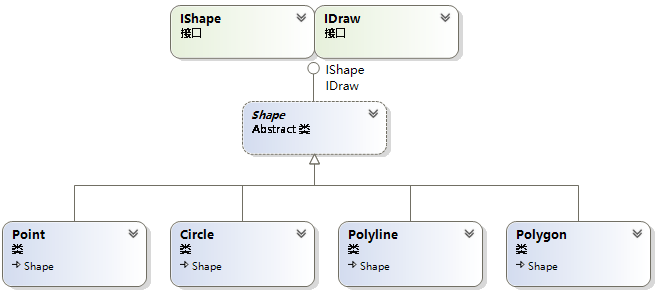
\includegraphics[scale=0.8]{chapter/csobject/graph.png}
	\caption{几何图形关系图}
	\label{fig:graph}
\end{figure}




\section{接口(interface)}
接口(interface)是指公开约定的属性或方法,接口是面向对象编程方法的重要概念。



\subsection{面向接口编程}

\subsection{接口跳转}


\section{封闭类(sealed class)}

\section{小结}      %% C# 之面向对象

%!TEX root = ../../clcxsj.tex

\chapter{测量基础函数设计}

本章我们将编写一些测量程序设计中常用的函数,用于以后的测绘算法之中。

\section{C\# 知识点}

C\# 是纯面向对象语言,也就是说所有的常量与方法都需要以类$class$为载体。

C\#中的类分为实例类与静态类。实例类需要用关键字 new 将类实例化,在一些与类的实例成员操作无关的
环境中,对类进行实例化的操作显得冗余,而静态类与类的静态成员可以很好的解决这个问题。 

如果我们分析C\#系统中的System.Math类,我们会发现常用的一些数学函数都被设计成了静态函数。因此,我们也如同System.Math类一样,
也将我们常用的测绘算法也用类名$SMath(SurveyMath)$命名,保存在$SMath.cs$文件中,
将常用的一些常量及方法定义也定义为静态成员。

示例代码如下所示:
\begin{lstlisting}
namespace ZXY
{
    public static class SMath
    {
        public const double PI=Math.PI;
        public const double TWOPI=2*Math.PI;
        public const double TODEG=180.0/PI; 
        public const double TORAD=PI/180.0;
        public const double TOSECOND=180.0*3600.0/PI;
    
        public static double DMStoRAD(double dmsAngle)
        {
            ......
        }
    
        public static double RADtoDMS(double radAngle)
        {
            ......
        }
    }
}
\end{lstlisting}

以上示例代码为了与其他的函数或符号相区别,也为了与其他的代码一起配合使用,
在此加入了自己的命名空间 ZXY (这是我用的名称空间,
你当然也可以根据自己的习惯或爱好命名适当的名称空间)。


\section{测绘常用算法设计}

\subsection{测绘算法中的常量}
角度、距离与高差是测量工程师工作的基本对象,度分秒形式的角度与弧度之间的转换是我们进行测量数据处理的基础。
为了方便的进行测量数据处理,我们首先需要定义一些常量,如上述示例代码所示,其中:

$PI$表示$\pi$, $TWOPI$表示$2\pi$;
$TODEG$表示$180/\pi$,用于将弧度化为度;
$TORAD$表示$\pi/180$,用于将度化为弧度;
$TOSECOND$表示$180*3600/\pi$,用于将弧度转换为秒。

在静态类SMath中我们采用常量const的形式定义了$\pi, 2\pi$等常用的数值,在 C\# 中 const类型的数据总是
静态的(static),而且是不需要static修饰符的。另外需注意,const类型的数据在声明时必须进行初始化,且其值
必须在编译时就能确定计算出。

\subsection{六十进制度分秒化弧度函数}

 在测量工程中角度的常用习惯表示法是度分秒的形式,
 在计算程序中测量工程人员也常将度分秒形式的角度用格式为xxx.xxxxx的形式表示,
 即以小数点前的整数部分表示度,小数点后两位数表示分,从小
 数点后第三位起表示秒。在计算机编程时所用的角度要以弧度表示的,因此需要
 设计函数相互转换。

 
角度化弧度函数的逻辑非常简单,许多测量编程人员将其写成如下的形式:

\begin{lstlisting}
public static double DMStoRAD(double dmsAngle)
{
   int d = (int)dmsAngle;
   dmsAngle = (dmsAngle - d) * 100.0;
   int m = (int)dmsAngle;
   double s = (dmsAngle - m) * 100.0;
   return (d + m / 60.0 + s / 3600.0) * TORAD;
}
\end{lstlisting}

但由于计算机中浮点数的表示方法的原因,以上函数并不能精确的将度分秒的角度转换为弧度。

 如角值为$1\degree 40'00''$,以1.4000浮点数输入,计算机将表示为1.3999999999999999的形式。
 这在计算机中并没有什么错误,但以上函数在提取角度的分秒时,提取到的m值为39,提取到的s值为
 99.999999999999,即我们提取到的角度为$1\degree 39'100''$,有 $40''$ 的角度误差,显然这是我们测绘工程人员不能接受的。
 
 有的软件设计人员在软件中发现这个问题后的处理的办法是让用户在角度后加减一秒,进行规避这种误差,显然,
 将软件人员的责任推给用户是极其不合适和不负责任的。还有许多的书籍中介绍了许多五花八门的处理方法,但奏效的小,
 不奏效的却很多,甚至有的将这么简单的算法逻辑变得逻辑十分复杂。
 
 虽然浮点数的表达不够精确,但我们知道在计算机中,整数的表达与计算却是精确的,因此在角度的度分秒值提取中,
 我们采用先将度分秒角度值提取为整数,然后再提取度分秒的运算方式进行计算,相应代码如下。
 
\begin{lstlisting}
public static double DMStoRAD(double dmsAngle)
{
    dmsAngle *= 10000; 
    int angle = (int)dmsAngle;
    int d = angle / 10000;
    angle -= d * 10000;
    int m = angle / 100;
    double s = dmsAngle - d * 10000 - m * 100;
    return (d + m / 60.0 + s / 3600.0) * TORAD;
}
\end{lstlisting}

首先将浮点形式的六十进制角度值乘以10000,如$1\degree 40'00''$表示为
13999.999999999999的形式,然后将其四舍五入取整到整秒,其值为14000。
再利用整数整除的精确算法将度(d)与分(m)提取出来。为了保持秒值的有效精度,
我们用精度无损失的dmsAngle值减去d与m的值提取出秒值(s)。 这样既可以正确提取出度
与分值,又可以保证秒值的有效精度。算法虽然简单,但确实需要保证这两个方面的需求。

 以上算法对于负的角度值的转换同样有效。

 考察精度(秒之后五位小数)是否足够:$39\degree 52'0.71672''$


\subsection{弧度函数化六十进制度分秒}

同样的道理,以下函数将不能正确的将一些弧度值转换为度分秒形式的角度值,
在某些情况下转换出的角度将出现$59'60''$或$59'59.9999''$的形式。

\begin{lstlisting}
public static double RADtoDMS(double radAngle)
{
    radAngle *= TODEG;
    int d = (int)radAngle;
    radAngle = (radAngle - d) * 60;
    int m = (int)radAngle;
    double s = (radAngle - m) * 60;
    return (d + m / 100.0 + s / 10000.0);
}
\end{lstlisting}

我们需要利用整数的精确表达能力与计算能力来进行转换,正确的代码如下:

\begin{lstlisting}
public static double RADtoDMS(double radAngle)
{
    radAngle *= TOSECOND;
    int angle = (int)radAngle; 
    int d = angle / 3600;
    angle -= d * 3600;
    int m = angle / 60;
    double s = radAngle - d * 3600 - m * 60;
    return (d + m / 100.0 + s / 10000.0);
}
\end{lstlisting}

首先我们将弧度转化为以秒为单位的double值,这个转换过程是精确的。其次,我们再将其四舍五入转换为
整秒值(虽然这个过程有精度损失,但我们仅用这个值提取度与分值)。再利用整数的精确计算能力提取度与分值,
最后用无精度损失的radAngle值减去度与分值就可以提取出正确的度分秒值了,而且也可以保证秒值的有效精度。

在这个算法中,将弧度值首先转换为秒为单位的值是关键,保证秒值的精确有效位数也很重要。

同样这个算法对负值也适用。

\subsection{角度规划函数}

在导线计算中,我们推算出的方位角值常常超出$0 -2\pi$的范围,这时我们就需要将角度规划到$0 -2\pi$范围内。
函数代码如下所示,rad的单位为弧度。

\begin{lstlisting}
 public static double To0_2PI(double rad)
 {
   int f = rad >= 0 ? 0 : 1;
   int n = (int)(rad / TWOPI);

   return rad - n * TWOPI + f * TWOPI;
 }
 \end{lstlisting}

 以上算法我们采用去整周角的算法,先计算出角度中所包含的$2\pi$个数n,
 然后减去这n个$2\pi$值。

 对于负的角度,以上算出的角度为负值,因此我们根据角度的符号性决定在角度为负值时再多加一个$2\pi$。


\subsection{坐标方位角计算}

在测量中,常常需要根据两点的坐标反算其坐标方位角,计算坐标方位角的关键是进行象限判断了。

已知A点与B点的坐标: A(xA, yA), B(xB, yB), 计算A->B的坐标方位角,函数名称定义为Azimuth,函数返回值为
两点的坐标方位角,单位为弧度,相应的代码如下:

\begin{lstlisting}
public static double Azimuth(double xA, double yA, double xB, double yB)
{
   double dx = xB - xA;
   double dy = yB - yA;
   return Math.Atan2(dy, dx) + (dy < 0 ? 1 : 0) * TWOPI;
}
\end{lstlisting}

在以上代码中,我们没有用常用的Math.Atan函数,该函数的取值范围为$-\pi /2 - \pi/2$,
取值区间为$\pi$,与坐标方位角的取值区间$2\pi$不相符,将其转换
到坐标方位角的取值范围内十分麻烦,而且还需要判断dx是否为0的情况。

查阅MSDN中对Math.Atan2函数的解释,我们发现其取值范围为$-\pi - \pi$,刚好为$2\pi$区间,
与坐标方位角的定义一致。且第一、第二象限的计算值为$0-\pi$, 与测量上的方位角定义一致;第三、第四象限的
计算值为$-\pi - 0$, 我们将其平移$2\pi$区间就可以将其转换到测量的第三、第四象限内,使其
与坐标方位角的定义一致。测量上第三、第四象限的判断条件为 $dy<0$,故只需要在Math.Atan2的计算值上
用三目运算符``?~ : ~''加上修正值$(dy < 0 ? 1 : 0) * TWOPI$就可以了。这样可以最大程度的保持代码的简洁了。

计算A、B两点的平距函数设计如下:
\begin{lstlisting}
public static double Distance(double xA, double yA, double xB, double yB)
{
    double dx = xB - xA;
    double dy = yB - yA;
    return Math.Sqrt(dx * dx + dy * dy);
}
\end{lstlisting}

可以看出,Azimuth函数与Distance函数十分相似,为了提高效率,也可以将这两个函数合并在一起,代码如下所示:

\begin{lstlisting}
public static double Azimuth(double xA, double yA, double xB, double yB, out double azimuth)
{
   double dx = xB - xA;
   double dy = yB - yA;
   azimuth = Math.Atan2(dy, dx) + (dy < 0 ? 1 : 0) * TWOPI;
   return Math.Sqrt(dx * dx + dy * dy);
}
\end{lstlisting}

在测量计算中,往往方位角的计算更加常用和重要,因此我们用out形式回带计算出的坐标方位角值,以函数返回值的形式返回两点的
平距,当不需要平距时,不接收函数返回值就可以了。


\section{算法的扩展}

六十进制的ddd.mmsss值十分利于角度数据的组织与输入,但不利于正式场景的角度展示。因此,在很多情况下我们需要
将角度表示为$23\degree 05'47.6324''$或$-23\degree 05'47.6324''$这种形式。
我们可以将前面的函数拷贝改写成如下形式的代码:

\begin{lstlisting}
public static string DMStoString(double dmsAngle)
{
    dmsAngle *= 10000; 
    int angle = (int)Math.Round(dmsAngle);
    int d = angle / 10000;
    angle -= d * 10000;
    int m = angle / 100;
    double s = dmsAngle - d * 10000 - m * 100;
    return string.Format("{0}`$\degree$`{1:00}`'`{2:00.0####}`''`", d, m, s);
}
\end{lstlisting}

第9行语句利用string的Format函数将度分秒值组合为字符串形式,其中的分值我们保持为两位整数数据,
不足两位的前面填0,同样的秒值整数部分也做这样的处理。秒值的小数部分保留五位小数,
如果后边为零的话自动去掉相应的小数位,但至少保持到0.1''。

这样在我们的代码中就存在着两份实现提取度分秒功能的代码了。在程序设计中,本着相同或相似的代码应尽可能的
只写一次的原则,我们应该将这部分功能代码独立出来,如下所示:

\begin{lstlisting}
public static void DMStoDMS(double dmsAngle, out int d, out int m, out double s)
{
    dmsAngle *= 10000; 
    int angle = (int)Math.Round(dmsAngle);
    d = angle / 10000;
    angle -= d * 10000;
    m = angle / 100;
    s = dmsAngle - d * 10000 - m * 100;
}
\end{lstlisting}

然后在DMStoRAD函数和DMStoString函数中进行调用,保持功能代码的唯一性。

\begin{lstlisting}
public static double DMStoRAD(double dmsAngle)
{
    DMStoDMS(dmsAngle, out int d, out int m, out double s);
    return (d + m / 60.0 + s / 3600.0) * TORAD;
}

public static string DMStoString(double dmsAngle)
{
    DMStoDMS(dmsAngle, out int d, out int m, out double s);
    return $"{d}`$\degree$`{m:00}`'`{s:00.0####}`''`";
}
\end{lstlisting}

第10行代码是C\# 6的语法,相对于前面的string.Format函数的写法,更加简洁。

同样的道理,我们对RADtoDMS函数与RADtoString函数也应做相应的处理,其代码如下:
\begin{lstlisting}
public static void RADtoDMS(double radAngle, out int d, out int m, out double s)
{
    radAngle *= TOSECOND;
    int angle = (int)Math.Round(radAngle);
    d = angle / 3600;
    angle -= d * 3600;
    m = angle / 60;
    s = radAngle - d * 3600 - m * 60;
}

public static double RADtoDMS(double radAngle)
{
    RADtoDMS(radAngle, out int d, out int m, out double s);
    return (d + m / 100.0 + s / 10000.0);
}

public static string RADtoString(double radAngle)
{
    RADtoDMS(radAngle, out int d, out int m, out double s);
    return $"{d}`$\degree$`{m:00}`'`{s:00.0####}`''`";
}
\end{lstlisting}



\subsection{对算法进行单元测试}

SMath项目中的各个函数是我们的基础测量算法函数,必须保证它们的正确性。
为此对其编写单元测试函数进行严格的测试。如果以后需要对这些算法进行优化,
执行这些单元测试函数也可确保优化后的算法正确性。

点击展开UnitTestSMath项目,鼠标右键点击原来的文件UnitTest1.cs,
在弹出的菜单中选择Rename命令,将其改名为UnitTestSMath.cs,
在弹出的确认对话框中选择按钮 `是(Y)'就可以将其中的类名改为UnitTestSMath了。

我们首先编写DMStoDMS函数的测试函数,其代码如下:

\begin{lstlisting}
//UnitTestSMath.cs文件内容
using System;
using Microsoft.VisualStudio.TestTools.UnitTesting;

namespace UnitTestSMath
{
    [TestClass]
    public class UnitTestSMath
    {
        [TestMethod]
        public void TestDMStoDMS()
        {
            ZXY.SMath.DMStoDMS(1.4, out int d, out int m, out double s);
            Assert.AreEqual(1, d);
            Assert.AreEqual(40, m);
            Assert.AreEqual(0, s, 1e-8);

            ZXY.SMath.DMStoDMS(-1.4, out d, out m, out s);
            Assert.AreEqual(-1, d);
            Assert.AreEqual(-40, m);
            Assert.AreEqual(0, s, 1e-8);

            ZXY.SMath.DMStoDMS(235.07492345, out d, out m, out s);
            Assert.AreEqual(235, d);
            Assert.AreEqual(7, m);
            Assert.AreEqual(49.2345, s, 1e-8);

            ZXY.SMath.DMStoDMS(-235.07492345, out d, out m, out s);
            Assert.AreEqual(-235, d);
            Assert.AreEqual(-7, m);
            Assert.AreEqual(-49.2345, s, 1e-8);
        }
    }
}
\end{lstlisting}

测试的原理非常简单,那就是已知一个值,让它经过一系列的运算得到期望的值。如果算法结果
与期望值相符,则测试通过,否则测试就不通过。

在Visual Studio系统中,单元测试的主要函数在Assert类中,其静态重载函数AreEqual
用于判断期望值(expected)与实际运算值(actual)是否相等。对于上述代码中d与m,由于
是整数,可以直接判断是否相等,而s是double类型,需给出一定的容错范围,不能直接判断
是否相等。

在测试代码中,我们分别用$1^{\degree} 40'$、$-1^{\degree} 40'$、
$235^{\degree} 07'49.2345''$、$-235^{\degree} 07'49.2345''$进行
测试,确保秒后第8位小数的准确性。

依次点击菜单栏上的Test -> Run -> All Tests 菜单项,在左侧的侧栏Test Explorer中
就可以显示测试结果,如图\ref{fig:AzimuthApp8}所示,图中左侧Test Explorer中测试项
显示为绿色,表明测试通过。

\begin{figure}[htbp]
    \centering
    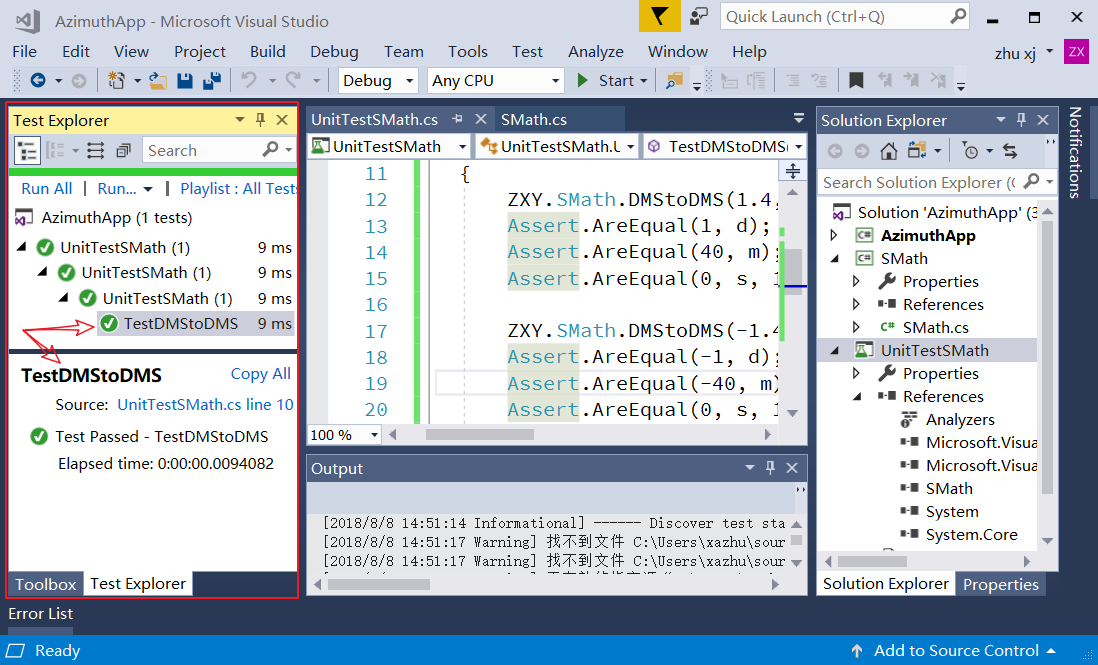
\includegraphics[scale=0.65]{chapter/surveybase/AzimuthApp8.png}
    \caption{执行单元测试成功的示意图}
    \label{fig:AzimuthApp8}
\end{figure}

如果我们将第30行代码中的-7改为-8,再执行测试命令,执行结果如图\ref{fig:AzimuthApp9},
图中左侧Test Explorer中测试项显示为红色的``×'',表明相应测试项未通过。

在Test Explorer下部显示了未通过测试的函数名称,位于源代码的哪一行,期望值是-8,
而实际值为-7。我们就可以根据这些信息去修正未通过测试的函数。

\begin{figure}[htbp]
    \centering
    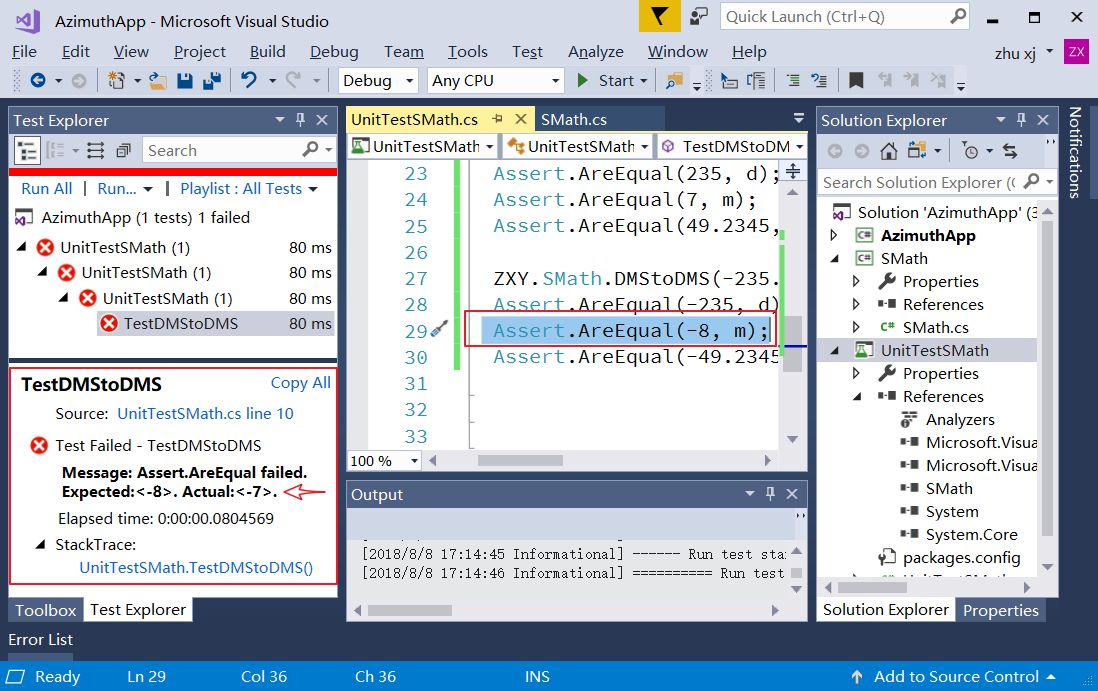
\includegraphics[scale=0.65]{chapter/surveybase/AzimuthApp9.png}
    \caption{执行单元测试失败的示意图}
    \label{fig:AzimuthApp9}
\end{figure}

由图\ref{fig:AzimuthApp8}与图\ref{fig:AzimuthApp9}可看出,测试通过,相应函数测试项
显示为绿色,测试项中之一不能通过,则相应函数测试项显示为红色。这就免去了我们人工再去比对的
环节,也利于机器的自动测试实施。


%%%%%%%%%%%%%%%%%%%%%%%%%%%%%%%%%%%%%
\section*{作业}

\begin{enumerate}
\item 以上DMStoString函数与RADtoString函数可以正确的将角度值中的度分秒值提取出来并
以更好阅读的字符串$23\degree 05'47.6324''$形式表达。但对于负的角度会表达为
$-23\degree -05'-47.6324''$形式,对于追求完美的某些程序员来讲这似乎有些不可接受,
他们仍然想将负的角度表达为$-23\degree 05'47.6324''$或$-0\degree 05'47.6324''$
形式。请试着改进以上的DMStoString与RADtoString函数。
    
\item 请用Math.Atan函数编写两点坐标反算坐标方位角的函数Azimuth。

\item 请将单元测试项目UnitTestSMath中的测试函数TestAzimuth与TestRADtoDMS等补充编写完整。
\end{enumerate}  %% 测量基础函数

%!TEX root = ../../clcxsj.tex

\chapter{面向对象程序设计原则}

面向对象程序设计的核心是类与接口,设计良好的程序需要遵循类的七个如下设计原则:

\begin{itemize}
	\item 开闭原则(OCP)
	\item 里氏代换原则
	\item 迪米特原则(最少知道原则)
	\item 单一职责原则
	\item 接口分隔原则
	\item 依赖倒置原则
	\item 组合/聚合复用原则
\end{itemize}

七大原则之间并不是相互孤立的,彼此之间是存在着一定关联,一个可以是另一个原则的加强或基础。
违反其中的某一个原则,可能同时也会违反其余的原则。

开闭原则是面向对象的可复用设计的基石。其他设计原则是实现开闭原则的手段和工具。

一般地,可以把这七个原则分成了以下两个部分:
\begin{itemize}
	\item 设计目标
	开闭原则、里氏代换原则、迪米特原则
	\item 设计方法
	单一职责原则、接口分隔原则、依赖倒置原则、组合/聚合复用原则
\end{itemize}


\section{开闭原则(OCP)}

\subsection{思想}
\emph{ 软件实体(模块,类,方法等)应该对扩展开放,对修改关闭。}

开闭原则英文为 The Open-Closed Principle,简称为OCP,是指在进行面向对象设计中,设计类或其他程序单位时,应该遵循:

\begin{itemize}

    \item 对扩展开放(open)

	某模块的功能是可扩展的,则该模块是扩展开放的。软件系统的功能上的可扩展性要求模块是扩展开放的。
    
    \item 对修改关闭(closed) 的设计原则

	某模块被其他模块调用,如果该模块的源代码不允许修改,则该模块修改关闭的。软件系统的功能上的稳定性,持续性要求模块是修改关闭的。

\end{itemize}

开闭原则是判断面向对象设计是否正确的最基本的原理之一。

根据开闭原则,在设计一个软件系统模块(类,方法)的时候,应该可以在不修改原有的模块(修改关闭)的基础上,能扩展其功能(扩展开放)。

\subsection{原因}

\begin{itemize}
\item{稳定性}

开闭原则要求扩展功能不修改原来的代码,这可以让软件系统在变化中保持稳定。

\item{扩展性}

开闭原则要求对扩展开放,通过扩展提供新的或改变原有的功能,让软件系统具有灵活的可扩展性。
遵循开闭原则的系统设计,可以让软件系统可复用,并且易于维护。
\end{itemize}

\subsection{实现方法}

为了满足开闭原则的对修改关闭原则以及扩展开放原则,应该对软件系统中的不变的部分加以抽象,在面向对象的设计中,

可以把这些不变的部分加以抽象成不变的接口,这些不变的接口可以应对未来的扩展;

接口的最小功能设计原则。根据这个原则,原有的接口要么可以应对未来的扩展;不足的部分可以通过定义新的接口来实现;

模块之间的调用通过抽象接口进行,这样即使实现层发生变化,也无需修改调用方的代码。

接口可以被复用,但接口的实现却不一定能被复用。

接口是稳定的,关闭的,但接口的实现是可变的,开放的。

可以通过对接口的不同实现以及类的继承行为等为系统增加新的或改变系统原来的功能,实现软件系统的柔性扩展。

好处:提高系统的可复用性和可维护性。

简单地说,软件系统是否有良好的接口(抽象)设计是判断软件系统是否满足开闭原则的一种重要的判断基准。现在多把开闭原则等同于面向接口的软件设计。

\subsection{代码示例}


\section{里氏替换原则(Liskov Substitution Principle ,LSP)}
所有引用基类的地方必须能透明地使用其派生类的对象。

也就是说,只有满足以下2个条件的OO设计才可被认为是满足了LSP原则:

不应该在代码中出现if/else之类对派生类类型进行判断的条件。

派生类应当可以替换基类并出现在基类能够出现的任何地方,或者说如果我们把代码中使用基类的地方用它的派生类所代替,代码还能正常工作。

以下代码就违反了LSP定义。


里氏替换原则(LSP)是使代码符合开闭原则的一个重要保证。

同时LSP体现了:

类的继承原则:如果一个派生类的对象可能会在基类出现的地方出现运行错误,则该派生类不应该从该基类继承,或者说,应该重新设计它们之间的关系。

动作正确性保证:从另一个侧面上保证了符合LSP设计原则的类的扩展不会给已有的系统引入新的错误。
示例:

里式替换原则为我们是否应该使用继承提供了判断的依据,不再是简单地根据两者之间是否有相同之处来说使用继承。

里式替换原则的引申意义:子类可以扩展父类的功能,但不能改变父类原有的功能。

具体来说:

子类可以实现父类的抽象方法,但不能覆盖父类的非抽象方法。
子类中可以增加自己特有的方法。
当子类的方法重载父类的方法时,方法的前置条件(即方法的输入/入参)要比父类方法的输入参数更宽松。
当子类的方法实现父类的方法时(重载/重写或实现抽象方法)的后置条件(即方法的输出/返回值)要比父类更严格或相等。

\section{迪米特原则(最少知道原则)(Law of Demeter ,LoD)}

迪米特原则(Law of Demeter)又叫最少知道原则(Least Knowledge Principle),可以简单说成:talk only to your immediate friends,只与你直接的朋友们通信,不要跟“陌生人”说话。

对于面向OOD来说,又被解释为下面两种方式:

1)一个软件实体应当尽可能少地与其他实体发生相互作用。

2)每一个软件单位对其他的单位都只有最少的知识,而且局限于那些与本单位密切相关的软件单位。

朋友圈的确定
“朋友”条件:

当前对象本身(this)
以参量形式传入到当前对象方法中的对象
当前对象的实例变量直接引用的对象
当前对象的实例变量如果是一个聚集,那么聚集中的元素也都是朋友
当前对象所创建的对象
任何一个对象,如果满足上面的条件之一,就是当前对象的“朋友”,否则就是“陌生人”。

迪米特原则的优缺点

迪米特原则的初衷在于降低类之间的耦合。由于每个类尽量减少对其他类的依赖,因此,很容易使得系统的功能模块功能独立,相互之间不存在(或很少有)依赖关系。

迪米特原则不希望类直接建立直接的接触。如果真的有需要建立联系,也希望能通过它的友元类来转达。因此,应用迪米特原则有可能造成的一个后果就是:系统中存在大量的中介类,这些类之所以存在完全是为了传递类之间的相互调用关系,这在一定程度上增加了系统的复杂度。

例如,购房者要购买楼盘A、B、C中的楼,他不必直接到楼盘去买楼,而是可以通过一个售楼处去了解情况,这样就减少了购房者与楼盘之间的耦合,如图所示。

\section{单一职责原则}
永远不要让一个类存在多个改变的理由。

换句话说,如果一个类需要改变,改变它的理由永远只有一个。如果存在多个改变它的理由,就需要重新设计该类。

单一职责原则原则的核心含意是:只能让一个类/接口/方法有且仅有一个职责。

为什么一个类不能有多于一个以上的职责?
如果一个类具有一个以上的职责,那么就会有多个不同的原因引起该类变化,而这种变化将影响到该类不同职责的使用者(不同用户):

一方面,如果一个职责使用了外部类库,则使用另外一个职责的用户却也不得不包含这个未被使用的外部类库。
另一方面,某个用户由于某个原因需要修改其中一个职责,另外一个职责的用户也将受到影响,他将不得不重新编译和配置。
这违反了设计的开闭原则,也不是我们所期望的。
职责的划分
既然一个类不能有多个职责,那么怎么划分职责呢?

Robert.C Martin给出了一个著名的定义:所谓一个类的一个职责是指引起该类变化的一个原因。

如果你能想到一个类存在多个使其改变的原因,那么这个类就存在多个职责。

\section{接口分隔原则(Interface Segregation Principle ,ISP)}
不能强迫用户去依赖那些他们不使用的接口。

换句话说,使用多个专门的接口比使用单一的总接口总要好。

它包含了2层意思:

接口的设计原则:接口的设计应该遵循最小接口原则,不要把用户不使用的方法塞进同一个接口里。如果一个接口的方法没有被使用到,则说明该接口过胖,应该将其分割成几个功能专一的接口。

接口的依赖(继承)原则:如果一个接口a继承另一个接口b,则接口a相当于继承了接口b的方法,那么继承了接口b后的接口a也应该遵循上述原则:不应该包含用户不使用的方法。 反之,则说明接口a被b给污染了,应该重新设计它们的关系。

如果用户被迫依赖他们不使用的接口,当接口发生改变时,他们也不得不跟着改变。换而言之,一个用户依赖了未使用但被其他用户使用的接口,当其他用户修改该接口时,依赖该接口的所有用户都将受到影响。这显然违反了开闭原则,也不是我们所期望的。

总而言之,接口分隔原则指导我们:

一个类对一个类的依赖应该建立在最小的接口上

建立单一接口,不要建立庞大臃肿的接口

尽量细化接口,接口中的方法尽量少

接口分隔原则的优点和适度原则
接口分隔原则从对接口的使用上为我们对接口抽象的颗粒度建立了判断基准:在为系统设计接口的时候,使用多个专门的接口代替单一的胖接口。

符合高内聚低耦合的设计思想,从而使得类具有很好的可读性、可扩展性和可维护性。

注意适度原则,接口分隔要适度,避免产生大量的细小接口。

单一职责原则和接口分隔原则的区别
单一职责强调的是接口、类、方法的职责是单一的,强调职责,方法可以多,针对程序中实现的细节;

接口分隔原则主要是约束接口,针对抽象、整体框架。

\section{依赖倒置原则(Dependency Inversion Principle ,DIP)}
A. 高层模块不应该依赖于低层模块,二者都应该依赖于抽象

B. 抽象不应该依赖于细节,细节应该依赖于抽象

C.针对接口编程,不要针对实现编程。

依赖:在程序设计中,如果一个模块a使用/调用了另一个模块b,我们称模块a依赖模块b。

高层模块与低层模块:往往在一个应用程序中,我们有一些低层次的类,这些类实现了一些基本的或初级的操作,我们称之为低层模块;另外有一些高层次的类,这些类封装了某些复杂的逻辑,并且依赖于低层次的类,这些类我们称之为高层模块。

依赖倒置(Dependency Inversion):
面向对象程序设计相对于面向过程(结构化)程序设计而言,依赖关系被倒置了。因为传统的结构化程序设计中,高层模块总是依赖于低层模块。

\section{组合/聚合复用原则(Composite/Aggregate Reuse Principle ,CARP)}
尽量使用组合/聚合,不要使用类继承。

即在一个新的对象里面使用一些已有的对象,使之成为新对象的一部分,新对象通过向这些对象的委派达到复用已有功能的目的。就是说要尽量的使用合成和聚合,而不是继承关系达到复用的目的。

组合和聚合都是关联的特殊种类。

聚合表示整体和部分的关系,表示“拥有”。组合则是一种更强的“拥有”,部分和整体的生命周期一样。

组合的新的对象完全支配其组成部分,包括它们的创建和湮灭等。一个组合关系的成分对象是不能与另一个组合关系共享的。

组合是值的聚合(Aggregation by Value),而一般说的聚合是引用的聚合(Aggregation by Reference)。

在面向对象设计中,有两种基本的办法可以实现复用:第一种是通过组合/聚合,第二种就是通过继承。

什么时候才应该使用继承
只有当以下的条件全部被满足时,才应当使用继承关系:

1)派生类是基类的一个特殊种类,而不是基类的一个角色,也就是区分"Has-A"和"Is-A"。只有"Is-A"关系才符合继承关系,"Has-A"关系应当用聚合来描述。

2)永远不会出现需要将派生类换成另外一个类的派生类的情况。如果不能肯定将来是否会变成另外一个派生类的话,就不要使用继承。

3)派生类具有扩展基类的责任,而不是具有置换掉(override)或注销掉(Nullify)基类的责任。如果一个派生类需要大量的置换掉基类的行为,那么这个类就不应该是这个基类的派生类。

4)只有在分类学角度上有意义时,才可以使用继承。

总的来说:

如果语义上存在着明确的"Is-A"关系,并且这种关系是稳定的、不变的,则考虑使用继承;如果没有"Is-A"关系,或者这种关系是可变的,使用组合。另外一个就是只有两个类满足里氏替换原则的时候,才可能是"Is-A" 关系。也就是说,如果两个类是"Has-A"关系,但是设计成了继承,那么肯定违反里氏替换原则。

错误的使用继承而不是组合/聚合的一个常见原因是错误的把"Has-A"当成了"Is-A" 。"Is-A"代表一个类是另外一个类的一种;"Has-A"代表一个类是另外一个类的一个角色,而不是另外一个类的特殊种类。
  %% 面向对象设计原则
%!TEX root = ../../clcxsj.tex

\chapter{WPF界面编写基础}

\section{WPF设计原则}

\subsection{概述}
WPF是Windows Presentation Foundation的简称,是一个与分辨率无关的 UI 框架。WPF底层是通过GPU图形硬件加速,基于矢量的呈现引擎。 WPF 提供一套完善的应用程序开发功能:Extensible Application Markup Language (XAML)、控件、数据绑定、布局、二维和三维图形、动画、样式、模板、文档、媒体、文本和版式。

\begin{figure}[htbp]
    \centering
    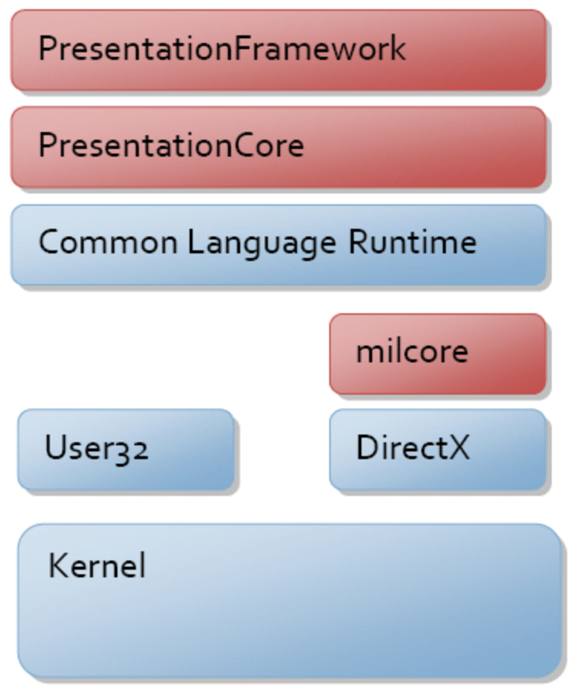
\includegraphics[scale=1]{chapter/uibase/wpf.png}
    \caption{WPF主要组件}
    \label{fig:wpf}
\end{figure}

 WPF的主要组件如图 \ref{fig:wpf} 所示,关系图的红色部分(PresentationFramework、PresentationCore 和 milcore)是 WPF 的主要代码部分。 WPF 中的所有显示都是通过 DirectX 引擎完成的,因此硬件和软件呈现高效。
 
 WPF 作为 .NET 类型的一个子集存在,大部分位于 System.Windows 命名空间中。 
 WPF设计思想是将界面标记描述与实现代码分离,从而实现界面设计(美工)与代码实现(开发人员)并行工作,提升开发效率。
 
界面标记描述使用 XAML,XAML的英文全称为 Extensible Application Markup Language, 翻译为中文为``可扩展应用程序标记语言'',XAML是派生自XML的可扩展应用程序标记语言,以声明形式实现应用程序的外观。 通常用它定义窗口、对话框、页面和用户控件,并填充控件、形状和图形。
  
现代软件开发如Android等,均采用xml等标记语言编写界面,因此WPF的思想以及XAML的方法很值得我们学习。
 
\subsection{WPF核心设计原则}

传统GDI方式与WinForm界面编写方式,均以鼠标拖拽为基础布置界面。

WPF界面设计的核心是:

\begin{enumerate}
    
\item 布局Grid化

摒弃鼠标拖拽这种过于简单方式布局界面,一般的应用将整个Window/Page用Grid进行网格化,再将各个控件按相应的网格行列号布置到相应位置上。

网格宽度与与高度则可设置为自动、指定像素值、按比例设置三种模式,从而控制在界面大小发生改变时,仍然使界面保持合理布局。

\item 数据交换绑定化

传统的界面与数据交换方式是直接向诸如Textbox的Text属性取值,并将其转换为相应数值,提供给相应算法进行计算,再将计算结果赋值到界面元素的相应属性中。

这种方式简单、直接。但在数据的容错处理上十分困难,从而导致程序的健壮性、功能正确性上也受到影响。

WPF为我们提供了数据绑定的方式进行数据交换。

\item 数据驱动界面化

WPF以数据为中心,数据驱动界面,而不是传统的事件驱动。

WPF是通过样式、控件模板、数据模板等方式实现了数据驱动界面。


\end{enumerate}



\section{XAML基本语法}

由于课时与篇幅的原因,此处对WPF的设计原理不做过多的论述,我们直接生成一个实例来分析XAML的语法。

\subsection{WPF项目结构}
我们基于 .net 6 生成一个默认的 WPF 项目,项目结构如图\ref{fig:wpfsln}所示:

\begin{figure}[htbp]
    \centering
    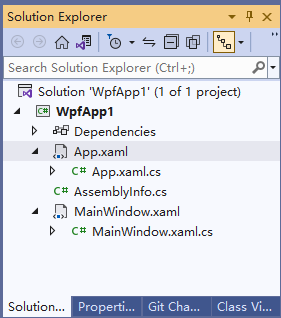
\includegraphics[scale=1]{chapter/uibase/wpfsln.png}
    \caption{WPF项目结构}
    \label{fig:wpfsln}
\end{figure}

项目中主要有两个文件App.xaml 与 MainWindow.xaml。每个xaml文件都有一个相应的扩展名为cs
的后台编码文件。

\subsection{项目中的xaml文件及含义}
App.xaml文件主要描述了项目的初始信息,代码如下:
\begin{lstlisting}[language=xml]
<Application x:Class="WpfApp1.App"
    xmlns="http://schemas.microsoft.com/winfx/2006/xaml/presentation"
    xmlns:x="http://schemas.microsoft.com/winfx/2006/xaml"
    xmlns:local="clr-namespace:WpfApp1"
    StartupUri="MainWindow.xaml">
    <Application.Resources>
    
    </Application.Resources>
</Application>
\end{lstlisting}

最主要的就是StartupUri 属性指定了该Application的启动地址是  "MainWindow.xaml" 文件。

 MainWindow.xaml文件描述了启动的主窗体,代码如下:

 \begin{lstlisting}[language=xml]
<Window x:Class="WpfApp1.MainWindow"
        xmlns="http://schemas.microsoft.com/winfx/2006/xaml/presentation"
        xmlns:x="http://schemas.microsoft.com/winfx/2006/xaml"
        xmlns:d="http://schemas.microsoft.com/expression/blend/2008"
        xmlns:mc="http://schemas.openxmlformats.org/markup-compatibility/2006"
        xmlns:local="clr-namespace:WpfApp1"
        mc:Ignorable="d"
        Title="MainWindow" Height="450" Width="800">
    <Grid>

    </Grid>
</Window>
\end{lstlisting}

文件中出现的 xmlns为文件中引入的命名空间,xmlns 为 xml namespace的缩写。

从这两个文件可以看出,每个xaml文件都是一颗xml的树,这棵树的根为Application、Window、Page等等。







%%%%%%%%%%%%%%%%%%%%%%%%%%%%%%%%%%%%%%
\section{WPF常用控件}

WPF控件基本上可以分为六类:

\begin{enumerate}
    \item 布局控件
    
    可以容纳多个控件或嵌套其它布局控件,用于在UI上组织和排列控件。如Grid、StackPanel、DockPanel等。
    
    \item 内容控件
    
    只能容纳一个其它控件或布局控件作为它的内容。Window、Button等均属于该类,是继承于类ContentControl。
    
    \item 带标题内容控件
    
    相当于一个内容控件,但可以加一个标题(Header),如GroupBox、TabItem等,是继承于类HeaderedContentControl。
    
    \item 条目控件
    
    可以显示一系列的数据,如ListBox、ComboBox等,它们继承于类ItemsControl。
    
    \item 带标题条目控件
    
    相当于一个条目控件加上一个标题显示区,如TreeViewItem、MenuItem等,用于显示层级关系数据,节点显示在Header区域,子节点显示在条目控件区域。它们继承于类HeaderedItemsControl。
    
    \item 特殊内容控件
    
    如TextBox容纳的字符串,TextBlock容纳的可自由控制格式的文本, Image容纳图片类型数据。
    
\end{enumerate}




%%%%%%%%%%%%%%%%%%%%%%%%%%%%%%%%%%%%%%
\section{坐标方位角计算图形界面程序编写}

前面我们编写了坐标方位角计算算法函数与角度弧度互相转换的函数。这节我们将借助于
WPF界面编写技术完成一个较为完整的图形界面的坐标方位角程序的编写。

\subsection{建立解决方案与项目}
启动Visual Studio(本书中所用版本为2017英文版),依次点击菜单File -> New -> Project...,
在弹出的对话框中按图\ref{fig:AzimuthApp1}所示输入新建项目名称、选择项目类型等。

\begin{figure}[htbp]
    \centering
    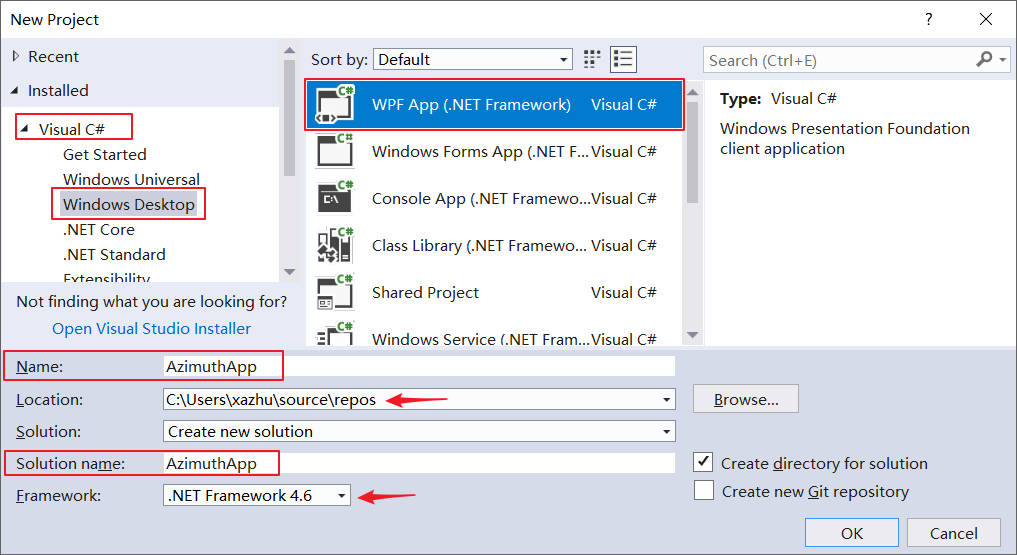
\includegraphics[scale=0.6]{chapter/surveybase/AzimuthApp1.png}
    \caption{新建项目示意图}
    \label{fig:AzimuthApp1}
\end{figure}

建好后的项目如图\ref{fig:AzimuthApp2}所示:

\begin{figure}[htbp]
    \centering
    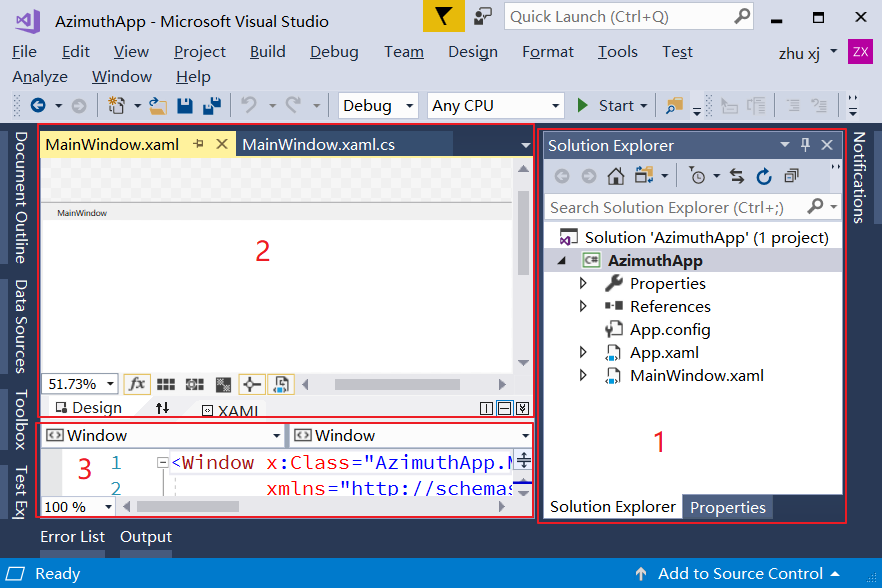
\includegraphics[scale=0.6]{chapter/surveybase/AzimuthApp2.png}
    \caption{方位角计算项目示意图}
    \label{fig:AzimuthApp2}
\end{figure}

由图\ref{fig:AzimuthApp2}可以看出,Visual Studio是以Solution、Project、File
的形式组织管理的。一个Solution可以包括一个至多个Project,一个Project中包含多个文件,
且一个Project编译为一个exe或dll文件,C\#中所有的对象与数据均以文件的形式组织。

图\ref{fig:AzimuthApp2}中的1区为Solution Explorer区,可对Project及File进行各种
操作。2、3区为代码与界面编写区,文件类型不同,呈现的内容也会不一样。

现代软件开发应遵循界面与算法分离的原则,因此我们再新建一类库项目SMath,用于
组织我们的算法,如图\ref{fig:AzimuthApp3}所示:

\begin{figure}[htbp]
    \centering
    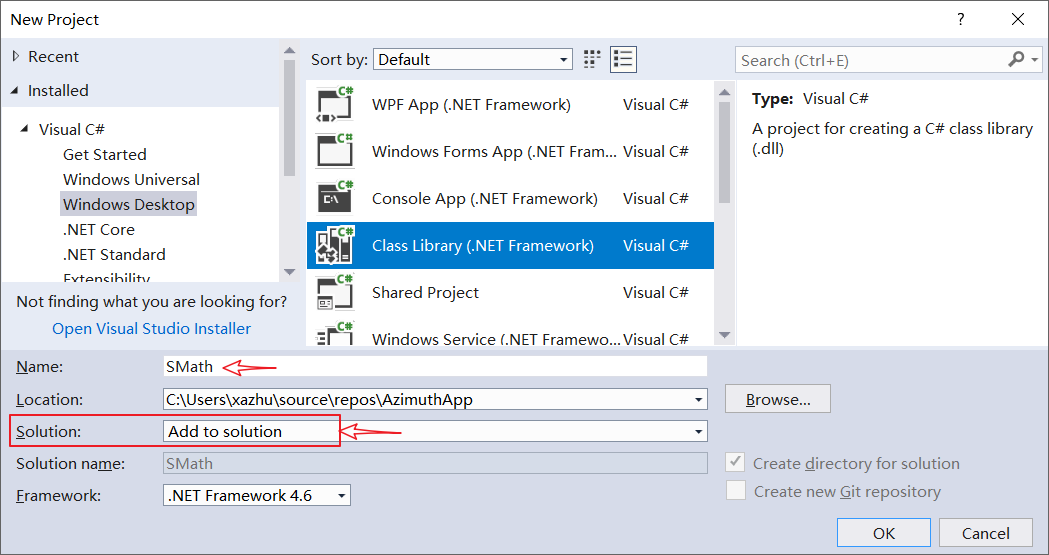
\includegraphics[scale=0.6]{chapter/surveybase/AzimuthApp3.png}
    \caption{新建类库项目示意图}
    \label{fig:AzimuthApp3}
\end{figure}

在该步操作中除了项目类型应选择Class Library之外,与图\ref{fig:AzimuthApp1}
不同的是此处Solution项应选择Add to solution而不是原来的 Create new solution。

现代软件开发的另一个原则是保证代码的可测试性,在增加类库项目后,
再增加一单元测试项目UnitTestSMath。鼠标右击图\ref{fig:AzimuthApp2}中的Solution Explorer区
中的Solution 'AzimuthApp'项,在弹出的右键快捷菜单中选择 Add,
在 Add 的下级菜单中选择 New Project..., 将弹出如图\ref{fig:AzimuthApp6}所示的添加单元测试项目的
对话框。

\begin{figure}[htbp]
    \centering
    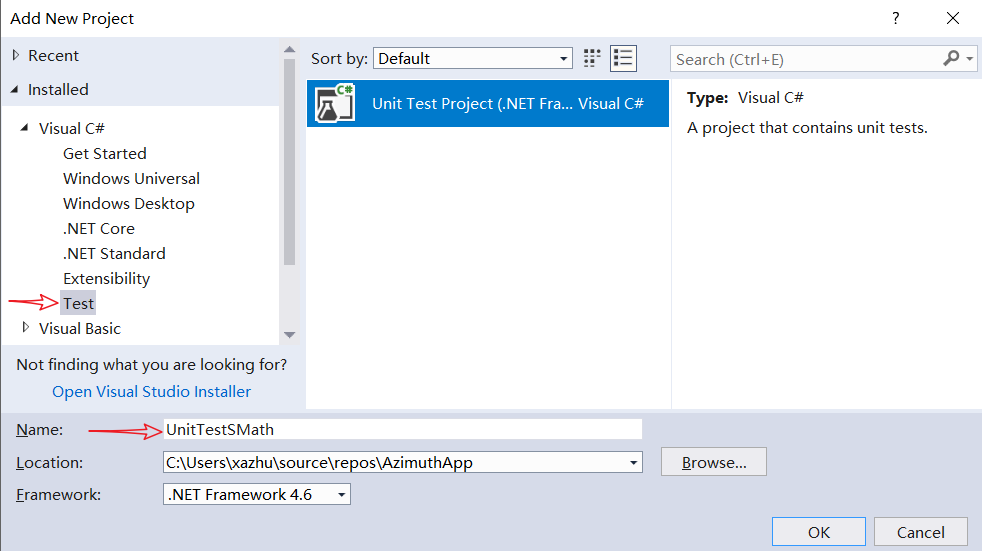
\includegraphics[scale=0.6]{chapter/surveybase/AzimuthApp6.png}
    \caption{添加单元测试项目示意图}
    \label{fig:AzimuthApp6}
\end{figure}

在图\ref{fig:AzimuthApp6}的操作中,应在左侧选择Test,在右边选择 Unit Test Project,

整个操作完成后,我们的解决方案Solution就拥有三个项目了,如图\ref{fig:AzimuthApp7}所示。
项目AzimuthApp为我们的界面编写项目,是启动项目(StartUp Project)。
项目SMath为我们的算法项目,项目UnitTestSMath为
对算法项目SMath进行单元测试的项目。

\begin{figure}[htbp]
\centering
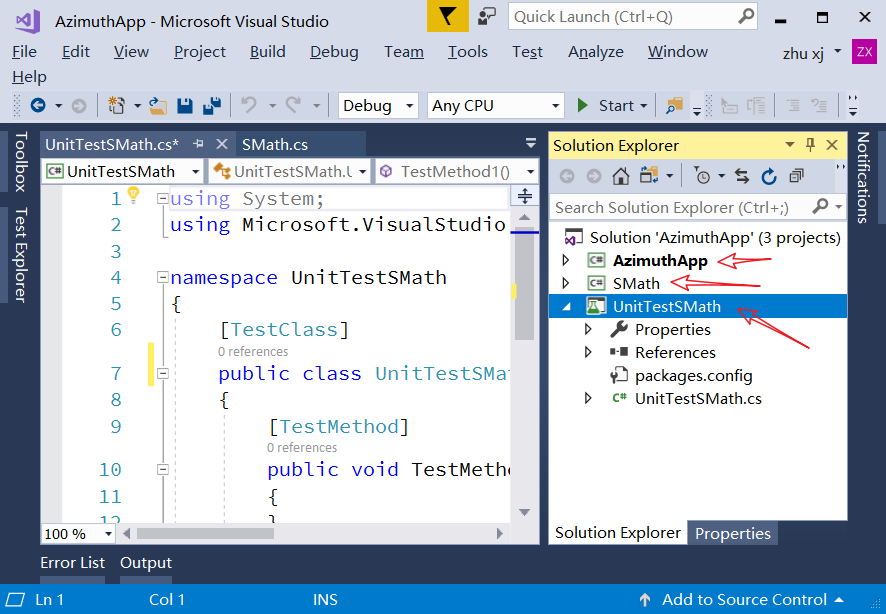
\includegraphics[scale=0.7]{chapter/surveybase/AzimuthApp7.png}
\caption{完整的Solution示意图}
\label{fig:AzimuthApp7}
\end{figure}

下面我们通过添加引用或参考(Add Reference)为三个项目建立关系。

SMath项目为基础算法,AzimuthApp需要用到其中的算法,因此应该向AzimuthApp项目
添加对SMath项目的引用。点击AzimuthApp项目将其展开,鼠标右击项目中的References
项,弹出如图\ref{fig:AzimuthApp4}所示的快捷菜单:

\begin{figure}[htbp]
\centering
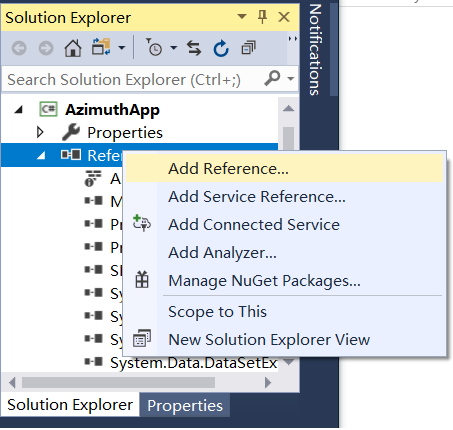
\includegraphics[scale=0.8]{chapter/surveybase/AzimuthApp4.png}
\caption{引用类库项目示意图}
\label{fig:AzimuthApp4}
\end{figure}

点击Add Reference...项,弹出如图\ref{fig:AzimuthApp5}所示的对话框。
在对话框左侧确保选中Projects,在右侧选中SMath项目,单击OK按钮就将引用添加完毕。
同样的方法向UnitTestSMath项目添加对SMath项目的引用。
\begin{figure}[htbp]
\centering
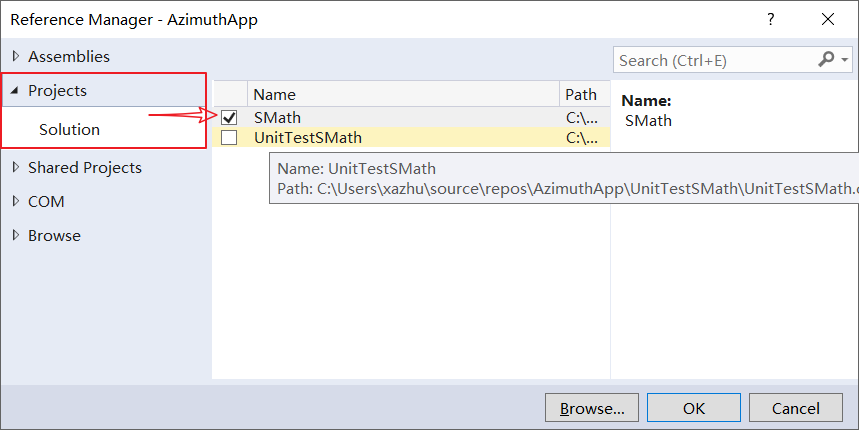
\includegraphics[scale=0.7]{chapter/surveybase/AzimuthApp5.png}
\caption{选择引用类库项目示意图}
\label{fig:AzimuthApp5}
\end{figure}

至此,我们的项目构建完成,整个程序的架构已经搭建好了。
在SMath项目中将原来的Class1.cs文件删除,新添一SMath.cs
文件,在SMath.cs文件中将我们前边讲解的SMath类加入其中,将各个函数组织进来,
对该项目执行构建(build)操作生成Dll类库文件,在另两个项目中就可以使用了。

\subsection{界面编写}

在确保基本算法的正确性后,我们就可以编写界面程序了。我们编写一简单界面,如图\ref{fig:AzimuthUI1}
所示。

\begin{figure}[htbp]
\centering
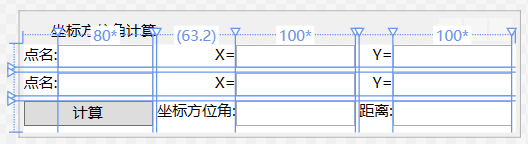
\includegraphics[scale=1]{chapter/surveybase/AzimuthUI1.png}
\caption{坐标方位角计算设计界面}
\label{fig:AzimuthUI1}
\end{figure}

相应的XAML设计代码如下:

\begin{lstlisting}[language=xml]
<Window x:Class="AzimuthApp.MainWindow"
    xmlns="http://schemas.microsoft.com/winfx/2006/xaml/presentation"
    xmlns:x="http://schemas.microsoft.com/winfx/2006/xaml"
    xmlns:d="http://schemas.microsoft.com/expression/blend/2008"
    xmlns:mc="http://schemas.openxmlformats.org/markup-compatibility/2006"
    xmlns:local="clr-namespace:AzimuthApp"
    mc:Ignorable="d"
    Title="坐标方位角计算" Height="100" Width="400">
    <Grid>
        <Grid.ColumnDefinitions>
            <ColumnDefinition Width="Auto"/>
            <ColumnDefinition Width="80*"/>
            <ColumnDefinition Width="3"/>
            <ColumnDefinition Width="Auto"/>
            <ColumnDefinition Width="100*"/>
            <ColumnDefinition Width="3"/>
            <ColumnDefinition Width="Auto"/>
            <ColumnDefinition Width="100*"/>
            <ColumnDefinition Width="3"/>
        </Grid.ColumnDefinitions>
        <Grid.RowDefinitions>
            <RowDefinition Height="Auto"/>
            <RowDefinition Height="3"/>
            <RowDefinition Height="Auto"/>
            <RowDefinition Height="3"/>
            <RowDefinition Height="Auto"/>
        </Grid.RowDefinitions>
        <TextBlock Text="点名:" Grid.Row="0" Grid.Column="0" />
        <TextBox x:Name="textBoxAName" Grid.Row="0" Grid.Column="1" />
        <TextBlock Text="X=" TextAlignment="Right" Grid.Row="0" Grid.Column="3"/>
        <TextBox x:Name="textBoxAX" Grid.Row="0" Grid.Column="4"/>
        <TextBlock Text="Y=" TextAlignment="Right" Grid.Row="0" Grid.Column="6"/>
        <TextBox x:Name="textBoxAY" Grid.Row="0" Grid.Column="7" />
        
        <TextBlock Text="点名:" Grid.Row="2" Grid.Column="0" />
        <TextBox x:Name="textBoxBName" Grid.Row="2" Grid.Column="1" />
        <TextBlock Text="X=" TextAlignment="Right" Grid.Row="2" Grid.Column="3"/>
        <TextBox x:Name="textBoxBX" Grid.Row="2" Grid.Column="4" />
        <TextBlock Text="Y=" TextAlignment="Right" Grid.Row="2" Grid.Column="6"/>
        <TextBox x:Name="textBoxBY" Grid.Row="2" Grid.Column="7" />
        
        <Button x:Name="buttonAzimuth" Content="计算" Grid.Row="5" 
            Grid.Column="0" Grid.ColumnSpan="2" Click="buttonAzimuth_Click"/>
        <TextBlock x:Name="textBlockAzimuth" 
            Text="坐标方位角:" TextAlignment="Right" Grid.Row="5" Grid.Column="3"/>
        <TextBox x:Name="textBoxAzimuth" Grid.Row="5" Grid.Column="4" />
        <TextBlock Text="距离:" TextAlignment="Right" Grid.Row="5" Grid.Column="6" />
        <TextBox x:Name="textBoxDistance" Grid.Row="5" Grid.Column="7" />
    </Grid>
</Window>
\end{lstlisting}

计算按钮的Click事件代码如下:
\begin{lstlisting}
private void buttonAzimuth_Click(object sender, RoutedEventArgs e)
{
    double.TryParse(textBoxAX.Text, out double xA);
    double.TryParse(textBoxAY.Text, out double yA);
    double.TryParse(textBoxBX.Text, out double xB);
    double.TryParse(textBoxBY.Text, out double yB);

    double distanceAB = ZXY.SMath.Azimuth(xA, yA, xB, yB, out double azimuthAB);

    textBoxAzimuth.Text = ZXY.SMath.RADtoString(azimuthAB);
    textBoxDistance.Text = distanceAB.ToString();
    textBlockAzimuth.Text = $"{textBoxAName.Text}->{textBoxBName.Text}坐标方位角:";
}
\end{lstlisting}

程序的运行结果如图\ref{fig:AzimuthUI2}所示。

\begin{figure}[htbp]
    \centering
    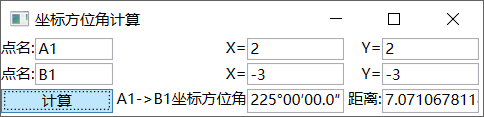
\includegraphics[scale=1]{chapter/surveybase/AzimuthUI2.png}
    \caption{坐标方位角计算运行界面}
    \label{fig:AzimuthUI2}
\end{figure}

\subsection{界面程序的优化}

WPF技术的核心是绑定(Binding),以上程序虽然简单,但也涉及数据与界面的交互问题。
我们对其界面稍加抽象,改写一下。

我们新建一个类AzimuthUI,其代码如下:
\begin{lstlisting}
using System.ComponentModel;

namespace AzimuthApp
{
    class AzimuthUI : INotifyPropertyChanged
    {
        public event PropertyChangedEventHandler PropertyChanged;
        public void RaisePropertyChanged(string propertyName)
        {
            if (PropertyChanged != null)
            {
                PropertyChanged.Invoke(this, new PropertyChangedEventArgs(propertyName));
            }
        }
        
        private string _AName = "";
        public string AName
        {
            get => _AName;
            set
            {
                _AName = value;
                RaisePropertyChanged("AName");
            }
        }
        
        private double _xA;
        public double XA
        {
            get => _xA;
            set
            {
                _xA = value;
                RaisePropertyChanged("XA");
            }
        }
        
        
        private double _yA;
        public double YA
        {
            get => _yA;
            set
            {
                _yA = value;
                RaisePropertyChanged("YA");
            }
        }
        
        private string _BName = "";
        public string BName
        {
            get => _BName;
            set
            {
                _BName = value;
                RaisePropertyChanged("BName");
            }
        }
        
        private double _xB;
        public double XB
        {
            get => _xB;
            set
            {
                _xB = value;
                RaisePropertyChanged("XB");
            }
        }
        
        private double _yB;
        public double YB
        {
            get => _yB;
            set
            {
                _yB = value;
                RaisePropertyChanged("YB");
            }
        }
        
        public string AzimuthName
        {
            get => $"{AName}->{BName}坐标方位角:";
        }
        
        private double _azimuthAB;
        public string AzimuthAB
        {
            get => ZXY.SMath.RADtoString(_azimuthAB);
        }
        
        private double _distanceAB;
        public double DistanceAB
        {
            get => _distanceAB;
        }
        
        public void CalAzimuthDistanceAB()
        {
            _distanceAB = ZXY.SMath.Azimuth(XA, YA, XB, YB, out _azimuthAB);
            RaisePropertyChanged("AzimuthAB");
            RaisePropertyChanged("DistanceAB");
            RaisePropertyChanged("AzimuthName");
        }
    }
}
\end{lstlisting}

界面代码做如下修改:
\begin{lstlisting}[language=XML]
    <TextBlock Text="点名:" Grid.Row="0" Grid.Column="0" />
    <TextBox x:Name="textBoxAName" Text="{Binding AName}" 
    Grid.Row="0" Grid.Column="1" />
    <TextBlock Text="X=" TextAlignment="Right"
    Grid.Row="0" Grid.Column="3"/>
    <TextBox x:Name="textBoxAX" Text="{Binding XA}" 
    Grid.Row="0" Grid.Column="4"/>
    <TextBlock Text="Y=" TextAlignment="Right" 
    Grid.Row="0" Grid.Column="6"/>
    <TextBox x:Name="textBoxAY" Text="{Binding YA}" 
    Grid.Row="0" Grid.Column="7" />
    
    <TextBlock Text="点名:" Grid.Row="2" Grid.Column="0" />
    <TextBox x:Name="textBoxBName" Text="{Binding BName}" 
    Grid.Row="2" Grid.Column="1" />
    <TextBlock Text="X=" TextAlignment="Right" Grid.Row="2" Grid.Column="3"/>
    <TextBox x:Name="textBoxBX" Text="{Binding XB}" 
    Grid.Row="2" Grid.Column="4" />
    <TextBlock Text="Y=" TextAlignment="Right" Grid.Row="2" Grid.Column="6"/>
    <TextBox x:Name="textBoxBY"  Text="{Binding YB}" 
    Grid.Row="2" Grid.Column="7" />
    
    <Button x:Name="buttonAzimuth" Content="计算" Grid.Row="5" 
    Grid.Column="0" Grid.ColumnSpan="2"
    Click="buttonAzimuth_Click"/>
    <TextBlock x:Name="textBlockAzimuth" 
    Text="{Binding AzimuthName, Mode=OneWay}" 
    TextAlignment="Right" Grid.Row="5" Grid.Column="3"/>
    <TextBox x:Name="textBoxAzimuth" Text="{Binding AzimuthAB, Mode=OneWay}" 
    Grid.Row="5" Grid.Column="4" />
    <TextBlock Text="距离:" TextAlignment="Right" Grid.Row="5" Grid.Column="6" />
    <TextBox x:Name="textBoxDistance" Text="{Binding DistanceAB, Mode=OneWay}"
    Grid.Row="5" Grid.Column="7" />
\end{lstlisting}

MainWindow窗体的后代代码做如下修改:

\begin{lstlisting}
namespace AzimuthApp
{
    public partial class MainWindow : Window
    {
        AzimuthUI azimuthUI;
        public MainWindow()
        {
            InitializeComponent();
            
            azimuthUI = new AzimuthUI();
            this.DataContext = azimuthUI;
        }
        
        private void buttonAzimuth_Click(object sender, RoutedEventArgs e)
        {
            azimuthUI.CalAzimuthDistanceAB();
        }
    }
}
\end{lstlisting}          %% wpf UI 基础, 将wpf基础、wpf数据绑定、wpf数据验证合并到这一章中,并以坐标方位角计算程序作为例子

%!TEX root = ../../clcxsj.tex

\chapter{高斯投影程序设计}

高斯投影是为解决球面与平面之间的坐标映射问题,即大地坐标(B,
L)与高斯平面直角坐标$(x,y)$之间的相互换算,以及不同带之间的高斯坐标
的换算问题。

高斯投影是我国1:50万以及更大比例尺地形图的数学基础,我国自1953年开始就采用,也是世界不少国家的地形图基础。
高斯投影在低纬度地区变形较大,在纬度30以下投影带的边缘部分变形值超过 1/1000 。
对低纬度地区地形图不是很适宜,对高纬度地区的地形图较好。

通用横墨卡托(Universal Transverse Mercator)简称为 UTM 投影,是横割圆柱投影,投影方法与高斯投影基本相同。
但每带中央子午线的长度比为 0.9996。
对中纬度地区与低纬度地区来讲,UTM投影优于高斯-克吕格投影。
UTM投影是目前美国、德国等60多个国家的国家基本地形图的数学基础。

本章将运用 \cs 编程语言编写一个通用的高斯投影程序,用于1954北京坐标系、1980西安坐标系、
WGS84坐标系以及CGCS2000大地坐标系或自定义参考椭球的高斯投影正反算与换带计算。


\section{高斯投影的数学模型}

为了编制正确而且高效的高斯投影与换带程序,我们首先需要分析高斯投影的数学模型,也就是我们
常说的算法。

本章所引用的公式来自:
孔祥元,郭际明,刘宗泉.大地测量学基础-2版.武汉:武汉大学出版社,2010.5,
以下将这本书简称为大地测量学基础或大地测量学。

\subsection{椭球基础}
投影是基于参考椭球进行的,所以首先需要分析参考椭球的计算。

高斯投影是在椭球的几何参数(长半轴a、短半轴b、扁率$\alpha$)确定的条件下,根据
给定的数学模型来进行计算的,我们首先分析这些计算公式与数学模型。

\begin{enumerate}

\item 基本公式

\begin{enumerate}
\item 扁率:
$$\alpha=\frac{a-b}{a}$$

\item 第一偏心率:
$$e=\sqrt{\frac{a^2-b^2}{a^2}}$$

\item 第二偏心率:
$$e'=\sqrt{\frac{a^{2}-b^{2}}{b^{2}}}$$

\item 子午圈曲率半径:
$$M=\frac{a(1-e^2)}{(1-e^2\sin ^2 B)^{\frac{3}{2}}}$$

\item 卯酉圈曲率半径:
$$N=\frac{a}{\sqrt{1-e^2\sin^2 B}}$$

\item 辅助符号:
$$t=\tan B\qquad\eta=e'\cos B$$
\end{enumerate}

\item 椭球面梯形图幅面积计算

$$P = \frac{b^2}{2}(L_2 - L_1) \left | \frac{\sin B}{1-e^2\sin^2 B} 
+ \frac{1}{2e}\ln \frac{1+e\sin B}{1-e\sin B}\right |_{B1} ^{B2} $$
公式引用自《大地测量学基础》第121页(4-140)。

$$P=b^2(L_2 - L_1) \left | sinB + \frac{2}{3}e^2 \sin ^3 B 
+ \frac{3}{5}e^4 \sin^5 B + \frac{4}{7}e^6 \sin ^7 B \right | _{B_1} ^{B_2}$$

公式引用自《大地测量学基础》第121页(4-142),该公式为(4-140)的展开式。

\item 子午线弧长
\begin{equation}
\label{eq:xx}
X=a_0 B - \frac{a_2}{2}\sin 2B + \frac{a_4}{4}\sin 4B
- \frac{a_6}{6} \sin 6B  + \frac{a_8}{8}\sin 8B
\end{equation}

式中:
\begin{equation}
\label{eq:xxaa}
\left  . \begin{aligned}
a_0 &= m_0 + \frac{m_2}{2} + \frac{3}{8}m_4 + \frac{5}{16}m_6 + \frac{35}{128}m_8  \\
a_2 &= \frac{m_2}{2} + \frac{m_4}{2} + \frac{15}{32}m_6 + \frac{7}{16}m_8  \\
a_4 &= \frac{m_4}{8} + \frac{3}{16}m_6 + \frac{7}{32}m_8  \\
a_6 &= \frac{m_6}{32} + \frac{m_8}{16}  \\
a_8 &= \frac{m_8}{128}
\end{aligned} \right \}
\end{equation}

式中$m_0, m_2, m_4, m_6, m_8$的值为:

\begin{equation}
\label{eq:xxmm}
\left . 
\begin{aligned}
m_0 &= a(1-e^2) \\
m_2 &= \frac{3}{2}e^2 m_0  \\
m_4 &= \frac{5}{4}e^2 m_2  = \frac{15}{8} e^4 m_0 \\
m_6 &= \frac{7}{6}e^2 m_4   = \frac{35}{16} e^6 m_0 \\
m_8 &= \frac{9}{8}e^2 m_6 = \frac{315}{128} e^8 m_0
\end{aligned} 
\right \}
\end{equation}

以上公式引用自《大地测量学基础》第115页(4-101)、(4-100)与(4-72).

将公式 \ref{eq:xxmm} 代入公式  \ref{eq:xxaa}可得到如下公式:

 \begin{equation}
\label{eq:xxaamm}
\left  . \begin{aligned}
a_0 &=(1 + \frac{3}{4} e^2 + \frac{45}{64} e^4 + \frac{175}{256} e^6 + \frac{11025}{16384} e^8) m_0  \\
a_2 &=(\frac{3}{4} e^2 + \frac{15}{16} e^4 + \frac{525}{512} e^6 + \frac{2205}{2048} e^8) m_0  \\
a_4 &=(\frac{15}{64} e^4 + \frac{105}{256} e^6 + \frac{2205}{4096} e^8) m_0  \\
a_6 &=(\frac{35}{512} e^6 + \frac{315}{2048} e^8) m_0  \\
a_8 &= \frac{315}{16384} e^8 m_0
\end{aligned} \right \}
\end{equation}

若令:
\begin{equation}
\label{eq:xxAAA}
\left  . \begin{aligned}
A_0 &=a_0 = (1 + \frac{3}{4} e^2 + \frac{45}{64} e^4 + \frac{175}{256} e^6 + \frac{11025}{16384} e^8) m_0  \\
A_2 &=-\frac{a2}{2} =-\frac{1}{2}  (\frac{3}{4} e^2 + \frac{15}{16} e^4 + \frac{525}{512} e^6 + \frac{2205}{2048} e^8) m_0  \\
A_4 &=\frac{a_4}{4}=\frac{1}{4} (\frac{15}{64} e^4 + \frac{105}{256} e^6 + \frac{2205}{4096} e^8) m_0  \\
A_6 &=-\frac{a_6}{6}=-\frac{1}{6} (\frac{35}{512} e^6 + \frac{315}{2048} e^8) m_0  \\
A_8 &= \frac{a_8}{8}=\frac{1}{8} \times \frac{315}{16384} e^8 m_0
\end{aligned} \right \}
\end{equation}

则子午线弧长公式 \ref{eq:xx}可以演变为如下公式:
\begin{equation}
\label{eq:AAAxxAAA}
X= A_0 B + A_2 \sin 2B + A_4 \sin 4B + A_6 \sin 6B  + A_8 \sin 8B
\end{equation}

公式 \ref{eq:AAAxxAAA} 将作为我们进行程序设计时进行子午线弧长与底点纬度计算的基本公式。

由公式 \ref{eq:xxAAA}看出,其值只与椭球的定义有关,一旦椭球的参数确定,这些值也就被确定。

% 或用很多书上都引用的公式:

% \begin{equation}
% \label{eq:CX}
% X=c[\beta_0 B + (\beta_2 \cos B + \beta_4 \cos^3 B + \beta_6 \cos^5 B + \beta_8 \cos^7 B) \sin B] 
% \end{equation}

% 式中 c 为极曲率半径,其值为: $c= a^2 / b$,
% $\beta_0, \beta_2, \beta_4, \beta_6, \beta_8$的值为:

% \begin{equation}
% \label{eq:CXC}
% \left .
% \begin{aligned}
% \beta_0 &= 1 - \frac{3}{4}e'^2 + \frac{45}{64}e'^4 - \frac{175}{256}e'^6 + \frac{11025}{16384}e'^8  \\
% \beta_2 &= \beta_0 -1  \\
% \beta_4 &= \frac{15}{32}e'^4 - \frac{175}{384}e'^6 + \frac{3675}{8192}e'^8   \\
% \beta_6 &= -\frac{35}{96}e'^6 + \frac{735}{2048}e'^8   \\
% \beta_8 &= \frac{315}{1024}e'^8
% \end{aligned} 
% \right \}
% \end{equation}

% 公式引用自《大地测量学基础》第115页(4-107)、与(4-108)。

% 可对公式\ref{eq:CXC}做进一步演化,令:
% \begin{equation}
% 	\label{eq:CXCC}
% 	\left .
% 	\begin{aligned}
% 		C_0 &= c \beta_0 = c(1 - \frac{3}{4}e'^2 + \frac{45}{64}e'^4 - \frac{175}{256}e'^6 + \frac{11025}{16384}e'^8) \\
% 		C_2 &= c \beta_2 = c(\beta_0 -1)                                                                              \\
% 		C_4 &= c \beta_4 = c(\frac{15}{32}e'^4 - \frac{175}{384}e'^6 + \frac{3675}{8192}e'^8)                         \\
% 		C_6 &= c \beta_6 = c(-\frac{35}{96}e'^6 + \frac{735}{2048}e'^8)                                               \\
% 		C_8 &= c \beta_8 = c(\frac{315}{1024}e'^8)
% 	\end{aligned}
% 	\right \}
% \end{equation}

% 则子午线弧长公式\ref{eq:CX}可演化为:

% \begin{equation}
% 	\label{eq:CXX}
% 	X=C_0 B + (C_2 \cos^2 B + C_4 \cos^4 B + C_6 \cos^6 B + C_8 \cos^8 B) \tan B
% \end{equation}

\subsection{高斯投影正算}

高斯投影正算就是将球面上一点的大地坐标 $(B, L)$ 投影为高斯平面直角坐标 $(x, y)$。

\item 高斯投影正算
\begin{equation}
\left .
\begin{aligned}
x&=X+\frac{l^2 N}{2}sinBcosB +\frac{l^4 N}{24}sinBcos^3B(5-t^2 +9\eta^2+4\eta^4) \\
  &+\frac{N}{720}sinBcos^5 B(61-58t^2 +t^4)l^6  \\
y&=l N cosB+\frac{l^3 N}{6}cos^3 B(1-t^2 +\eta^2 ) \\
        &+\frac{l^5 N}{120}cos^5 B (5-18t^2+t^4 +14\eta^2 -58\eta^2t^2)
\end{aligned}
 \right \}
\end{equation}

公式引用自《大地测量学基础》第169页(4-367)。

\item 高斯投影反算

\begin{equation}
\left  .
\begin{aligned}
B&=B_f - \frac{t_f}{2M_f N_f }y^2 +\frac{t_f}{24 M_f N_f ^3}
(5 + 3t_f ^2  + \eta_f ^2 - 9\eta_f ^2 t_f^2)y^4 \\
 &- \frac{t_f}{720 M_f N_f ^5}(61 + 90t_f ^2 + 45t_f ^4)y^6 \\
l&=\frac{1}{N_f cosB_f}y - \frac{1}{6N_f ^3 cosB_f}(1 + 2t_f ^2 + \eta_f ^2)y^3  \\
 &+ \frac{1}{120N_f ^5 cosB_f}(5 + 28t_f ^2 + 24t_f ^4 + 6\eta_f ^2 +8\eta_f ^2 t_f ^2)y^5
\end{aligned} 
\right \}
\end{equation}

公式引用自《大地测量学基础》第171页(4-383)。


\item 平面子午线收敛角计算

利用$(B, l)$计算公式如下:
$$\gamma = l \cdot \sin B  + \frac{l^3}{3} \sin B \cos ^2 B \cdot (1 + 3 \eta^2 + 2 \eta^4)
+ \frac{ l^5}{15}\sin B \cos ^4 B \cdot (2 - t^2)$$

公式引用自《大地测量学基础》第181页(4-408)。

利用$(x, y)$计算公式如下:

$$\gamma = \frac{1}{N_f}t_f y - \frac{1+t_f ^2 - \eta_f ^2}{3N_f ^3}t_f y^3
+ \frac{2+5t_f^2+3t_f^4}{15N_f ^5}t_fy^5$$

公式引用自《大地测量学基础》第182页(4-410)。

\item 长度比计算

利用$(B, l)$计算公式如下:
$$m=1+\frac{l^2}{2} \cos ^2 B(1+\eta^2) + \frac{l^4}{24}\cos ^4 B(5-4t^2)$$

公式引用自《大地测量学基础》第189页(4-447)。

利用$(x, y)$计算公式如下:

$$m=1+\frac{y^2}{2R^2} + \frac{y^4}{24R^4}$$

式中$R=\sqrt{MN}$,公式引用自《大地测量学基础》第189页(4-451)。

\end{enumerate}

\section{程序功能分析与设计}

\subsection{高斯投影的主要内容}
\begin{enumerate}
    \item 坐标正算:将点的大地坐标转换成高斯投影平面直角坐标。
    \item 坐标反算:将点的高斯投影平面直角坐标转换成大地坐标。
    \item 换带计算:将某带的点的高斯投影平面直角坐标转换成邻带或某中央
    子午线经度的高斯投影平面直角坐标。
    \item 其他计算:计算子午线收敛角、长度比等。
\end{enumerate}

\subsection{参考椭球类的设计}

分析以上各个计算公式发现,如果椭球长半轴与扁率确定,参考椭球的第一偏心率$e$、
第二偏心率$e'$,子午线弧长计算的辅助计算参数$(m_0, m_2, m_4, m_6, m_8)$与
$(a_0, a_2, a_4, a_6, a_8)$也就确定了,其中的$(m_0, m_2, m_4, m_6, m_8)$
作为计算$(a_0, a_2, a_4, a_6, a_8)$的值使用过一次。也就是说这些参数对于某一种确定的
参考椭球是常数。而$(M,N,t,\eta)$则是纬度$B$的函数。

我们新建一 WPF 项目,命名为GaussProj,程序中我们将应用WPF技术编写图形界面。

在高斯投影中由于要处理角度与点等数据,我们可将前面的角度处理函数DMS2RAD、RAD2DMS
与SPoint点类拷贝到当前项目中来,也可以将其打包成一 Class Library(.NET Framework)
即类库文件引用到当前项目中,在当前项目中尽量不修改前面的各个功能代码。

基于上一小节的分析,我们新建一椭球类$(Spheroid)$,在其中我们定义以上与椭球类型
相关的元素。代码如下所示:

\begin{lstlisting}
namespace GaussProj
{
    /// <summary>
    /// 参考椭球
    /// </summary>
    public class Spheroid
    {
        /// <summary>
        /// 长半轴
        /// </summary>
        public double a { get; set; }

        /// <summary>
        /// 短半轴
        /// </summary>
        public double b { get; set; }

        /// <summary>
        /// 扁率分母
        /// </summary>
        public double f { get; set; }  //(a-b)/a = 1/f

        /// <summary>
        /// 第一偏心率的平方
        /// </summary>
        public double e2 { get; set; }

         /// <summary>
        /// 第二偏心率的平方
        /// </summary>
        public double eT2 { get; set; }

        //计算子午线弧长时的各个系数项
        private double a0;
        private double a2;
        private double a4;
        private double a6;
        private double a8;
    }
}
\end{lstlisting}

在各项计算中,第一偏心率与第二偏心率的直接使用较少,其平方值用的较多,因此在
Spheroid类我们直接用其平方值。

 在Spheroid类中我们可以如下直接定义构造函数用于初始化其各个字段(Field):
  \begin{lstlisting}
/// <summary>
/// 构造函数
/// </summary>
private Spheroid(double semimajor_axis, double inverse_flattening)
{
    this.a = semimajor;
    this.f =  inverse_flattening;
    ...................................................
}
\end{lstlisting}

但这样我们可能无法为已知的一些参考椭球直接提供参数,所以我们将构造函数定义
为 private,让用户无法通过new直接创建实例化对象。我们设计类的静态函数
Create**** 来创建类Spheroid的实例化对象,其代码如下:

 \begin{lstlisting}
/// <summary>
/// 构造函数
/// </summary>
private Spheroid(){}

/// <summary>
/// 初始化椭球参数的内部函数
/// </summary>
private void Init(double semimajor_axis, double inverse_flattening)
{
    this.a = semimajor_axis; this.f = inverse_flattening;
    b = a * (1 - 1 / f);

    e2 = 1 - b / a * b / a;
    eT2 = a / b * a / b - 1;

    double m0 = a * (1 - e2);
    double m2 = 3.0 / 2.0 * e2 * m0;
    double m4 = 5.0 / 4.0 * e2 * m2;
    double m6 = 7.0 / 6.0 * e2 * m4;
    double m8 = 9.0 / 8.0 * e2 * m6;

    a0 = m0 + m2 / 2.0 + 3.0 / 8.0 * m4 + 5.0 / 16.0 * m6
                  + 35.0 / 128.0 * m8;
    a2 = m2 / 2.0 + m4 / 2.0 + 15.0 / 32.0 * m6 + 7.0 / 16.0 * m8;
    a4 = m4 / 8.0 + 3.0 / 16.0 * m6 + 7.0 / 32.0 * m8;
    a6 = m6 / 32.0 + m8 / 16.0;
    a8 = m8 / 128.0;
}

public static Spheroid CreateBeiJing1954()
{
    Spheroid spheroid = new Spheroid();
    spheroid.Init(6378245, 298.3);
    return spheroid;
}

public static Spheroid CreateXian1980()
{
    Spheroid spheroid = new Spheroid();
    spheroid.Init(6378140, 298.257);
    return spheroid;
}

public static Spheroid CreateWGS1984()
{
    Spheroid spheroid = new Spheroid();
    spheroid.Init(6378137, 298.257223563);
    return spheroid;
}

public static Spheroid CreateCGCS2000()
{
    Spheroid spheroid = new Spheroid();
    spheroid.Init(6378137, 298.257222101);
    return spheroid;
}

public static Spheroid CreateCoordinateSystem(double semimajor_axis,
      double inverse_flattening)
{
    Spheroid spheroid = new Spheroid();
    spheroid.Init(semimajor_axis, inverse_flattening);
    return spheroid;
}
\end{lstlisting}

这种将构造函数设为private,通过静态函数来创建实例化对象的技术在软件设计中
会经常用到。同时在设计类的方法时,应注意访问权限的设置,如上面代码中Init函数,
在类中用于初始化椭球的各项几何参数,并不需要在类外来调用它,所以我们将其设置为
private权限。

\subsection{高斯投影正算功能的实现}
有了类Spheroid的设计,我们先来完成高斯投影正算功能。
为了避免在计算中频繁的进行度分秒与弧度之间的转换问题,
我们设定除了特别声明之外,在类Spheroid中所用的角度均为弧度。

我们将高斯投影正算的函数名称定义为 BLtoXY,其设计如下:

\begin{lstlisting}
/// <summary>
/// 高斯投影正算
/// </summary>
/// <param name="B">纬度,单位:弧度</param>
/// <param name="L">经度,单位:弧度</param>
/// <param name="L0">中央子午线经度,单位:弧度</param>
/// <param name="x">高斯平面x坐标</param>
/// <param name="y">高斯平面y坐标</param>
public void BLtoXY(double B, double L, double L0,
    out double x, out double y)
{
    ......................................
}
\end{lstlisting}

由于函数的返回值为两个值x与y,无法以函数的返回值return的形式返回计算结果,
所以我们用函数参数 out 的形式将计算结果返回。

 由前面的高斯投影正算公式分析可知,高斯投影正算的计算较为简单,没有复杂的逻辑,
 先计算经差,然后计算子午线弧长后就可以直接写计算坐标x,y的算法了。
 但公式较为复杂,极容易写错,公式中具有大量的平方、四次方等变量。因此在编程时
 应将这些变量命名为与其相似的形式并提前计算。相关代码如下:

\begin{lstlisting}
/// <summary>
/// 计算子午线弧长
/// </summary>
/// <param name="B">纬度(单位:弧度)</param>
/// <returns>子午线弧长</returns>
private double funX(double B)
{
    return a0 * B - a2 / 2.0 * Math.Sin(2 * B)
        + a4 / 4.0 * Math.Sin(4 * B)
        - a6 / 6.0 * Math.Sin(6 * B)
        + a8 / 8.0 * Math.Sin(8 * B);
}

private double funN(double sinB)
{
    return a / Math.Sqrt(1 - e2 * sinB * sinB);
}

/// <summary>
/// 高斯投影正算
/// </summary>
/// <param name="B">纬度,单位:弧度</param>
/// <param name="L">经度,单位:弧度</param>
/// <param name="L0">中央子午线经度,单位:弧度</param>
/// <param name="x">高斯平面x坐标</param>
/// <param name="y">高斯平面y坐标</param>
public void BLtoXY(double B, double L, double L0,
    out double x, out double y)
{
    double l = L - L0; //计算经差

    double sinB = Math.Sin(B);
    double cosB = Math.Cos(B);
    double cosB2 = cosB * cosB;
    double cosB4 = cosB2 * cosB2;
    double t = Math.Tan(B);
    double t2 = t * t;
    double t4 = t2 * t2;
    double g2 = eT2 * cosB * cosB;
    double g4 = g2 * g2;
    double l2 = l * l;
    double l4 = l2 * l2;

    double X = funX(B); //计算子午线弧长
    double N = funN(sinB);

    x = X + 0.5 * N * sinB * cosB * l2 * (1
        + cosB2 / 12.0 * (5 - t2 + 9 * g2 + 4 * g4) * l2
        + cosB4 / 360.0 * (61 - 58 * t2 + t4) * l4);


   y = N * cosB * l * (1
        + cosB2 * (1 - t2 + g2) * l2 / 6.0
        + cosB4 * (5 - 18 * t2 + t4 + 14 * g2 - 58 * g2 * t2)
                * l4 / 120.0);
}
\end{lstlisting}

利用 BLtoXY 函数就可以进行高斯投影正算了,其算法流程为:

\begin{lstlisting}
//创建克拉索夫斯基参考椭球
Spheroid  spheroid = Spheroid.CreateBeiJing1954();

//传入点的纬度B、经度与中央子午线经度,单位为弧度
double B = ZXY.SMath.DMS2RAD(21.58470845);
double L = ZXY.SMath.DMS2RAD(113.25314880);
double L0 = ZXY.SMath.DMS2RAD(111);
double x, y;

spheroid.BLtoXY(B, L, L0, out x, out y);
\end{lstlisting}

点的纬度、经度为:$ B = 21 \degree 58'47.0845'',  L= 113\degree 25'31.4880''$,
中央子午线经度为:$L0 = 111\degree$,
计算出的坐标为:$x=2433586.692, y=250547.403$, 坐标y为点的自然坐标,
未加常数500km与带号。

\subsection{高斯投影反算功能的实现}
由高斯投影反算公式分析,在反算时需要首先计算底点纬度。底点纬度需要由
子午线弧长公式进行反算,由该公式可以看出,已知X=x时,这个函数在计算B值时它
并不是一个线型函数,不能直接计算。解决这类问题的计算方法就是迭代计算,我们将公式
进行变换,如下所示:

$$B= (X + \frac{a_2}{2}\sin 2B - \frac{a_4}{4}\sin 4B
+ \frac{a_6}{6} \sin 6B  - \frac{a_8}{8}\sin 8B)/a_0$$

在该公式中,两边都有B,我们将公式右边的B赋初始值$B_0=X/a_0$代入可以
计算出新的$B$值,循环进行计算,由于该迭代收敛,两值之差 $B - B_0$ 在一定范围内时
我们认为其值 $B$ 即为我们的解。

因此底点纬度计算函数设计为:

\begin{lstlisting}
/// <summary>
/// 计算底点纬度
/// </summary>
/// <param name="x">高斯平面坐标x</param>
/// <returns>底点纬度</returns>
private double funBf(double x)
{
    double sinB, sin2B, sin4B, sin6B, sin8B;
    double Bf0 = x / a0, Bf = 0; //子午线弧长的初值
    int i = 0;
    while (i < 10000)//设定最大迭代次数
    {
        sinB = Math.Sin(Bf0);
        sin2B = Math.Sin(2 * Bf0);
        sin4B = Math.Sin(4 * Bf0);
        sin6B = Math.Sin(6 * Bf0);
        sin8B = Math.Sin(8 * Bf0);
        Bf = (x
        + a2 * sin2B / 2
        - a4 * sin4B / 4
        + a6 * sin6B / 6
        - a8 * sin8B / 8) / a0;

        if (Math.Abs(Bf - Bf0) < 1e-10) //计算精度
            return Bf;
        else
        {
            Bf0 = Bf;
            i++;
        }
    }
    return -1e12;
}
\end{lstlisting}

 在底点纬度计算出以后,高斯投影反算计算就没有难度了。
 我们将函数名命名为 XYtoBL,其函数设计为:
 \begin{lstlisting}
public void XYtoBL(double x, double y, double L0,
    out double B, out double L)
{
   double Bf = funBf(x);

    double cosBf = Math.Cos(Bf);
    double gf2 = eT2 * cosBf * cosBf;
    double gf4 = gf2 * gf2;
    double tf = Math.Tan(Bf);
    double tf2 = tf * tf;
    double tf4 = tf2 * tf2;
    double sinB = Math.Sin(Bf);
    double Nf = funN(sinB);
    double Mf = funM(sinB);
    double Nf2 = Nf * Nf;
    double Nf4 = Nf2 * Nf2;
    double y2 = y * y;
    double y4 = y2 * y2;

    B = Bf + tf * y2 / Mf / Nf * 0.5 * (
       -1.0
      + y2 * (5.0 + 3.0 * tf2 + gf2 - 9.0 * gf2 * tf2) / 12.0 / Nf2
      - y4 * (61.0 + 90.0 * tf2 + 45.0 * tf4) / 360.0 / Nf4);

   double l = y / Nf / cosBf * (
        1.0
      - y2 / 6.0 / Nf2 * (1.0 + 2.0 * tf2 + gf2)
     + y4 / 120.0 / Nf4
     * (5.0 + 28.0 * tf2 + 24.0 * tf4 + 6.0 * gf2 + 8.0 * gf2 * tf2));

    L = L0 + l;
}
\end{lstlisting}

该函数中还有Nf与Mf需要计算,Nf的计算同前面的funN函数,Mf的计算函数为
 \begin{lstlisting}
private double funM(double sinB)
{
    return a * (1 - e2) * Math.Pow(1 - e2 * sinB * sinB, -1.5);
}
\end{lstlisting}

 有了高斯投影反算函数 XYtoBL, 就可以比较容易的写出其反算示例了,如以下代码所示:

\begin{lstlisting}
//创建克拉索夫斯基参考椭球
Spheroid  spheroid = Spheroid.CreateBeiJing1954();

//传入点的X、Y坐标与中央子午线经度(单位为弧度)
double x=2433586.692, y=250547.403;
double L0 = ZXY.SMath.DMS2RAD(111);

double B, L;
spheroid.XYtoBL(x, y, L0, out B, out L);
//B= ZXY.SMath.RAD2DMS(B);
//L= ZXY.SMath.RAD2DMS(L);
\end{lstlisting}

传入的y坐标应为真实坐标值,应不包括500km与带号等。
如果计算的经纬度需向界面展示,还应像上述代码后两行所示将其值转换为
度分秒形式。

计算出的点的纬度与经度为:
$B=21 \degree 58'47.0845'', L=113\degree 25'31.4880''$

计算点的子午线收敛角与计算某点处的长度变形值均比较简单,可以在正算或反算时将其同时
计算出,大家可以自己练习完成,在此就不再讲述了。

\subsection{换带计算}
换带计算其实质就是变换坐标系的中央子午线位置。因此首先应根据点的坐标
反算出点的经纬度,然后再根据新的坐标系中央子午线位置计算出点在
新的坐标系中的高斯平面坐标。

也就是先反算,再正算,注意此处的反算与正算的中央子午线经度值是不一样的。

该函数我们命名为 XYtoXY,其设计为如下代码:

\begin{lstlisting}
/// <summary>
/// 高斯投影换带
/// </summary>
/// <param name="ox">点在源坐标系的x坐标</param>
/// <param name="oy">点在源坐标系的y坐标</param>
/// <param name="oL0">源坐标系的中央子午线经度,单位:弧度</param>
/// <param name="nL0">目标坐标系的中央子午线经度,单位:弧度</param>
/// <param name="nx">点在目标坐标系的x坐标</param>
/// <param name="ny">点在目标坐标系的y坐标</param>
public void XYtoXY(double ox, double oy,
    double oL0, double nL0,
   out double nx, out double ny)
{
    double B, L;
    XYtoBL(ox, oy, oL0, out B, out L); //高斯投影反算
    BLtoXY(B, L, nL0, out nx, out ny); //高斯投影正算
}
\end{lstlisting}

高斯投影换带的外部调用可以按如下方式写:

\begin{lstlisting}
double oldX = 3275110.535, oldY = 235437.233;

double oldL0 = ZXY.SMath.DMS2RAD(117);
double newL0 = ZXY.SMath.DMS2RAD(120);

double newX, newY;
Spheroid  spheroid = Spheroid.CreateBeiJing1954();
spheroid.XYtoXY(oldX, oldY, oldL0, newL0, out newX, out newY);
\end{lstlisting}

计算出的点在新坐标系下的坐标为(3272782.315, -55299.545)。

至此,我们已经完成了高斯投影的全部计算功能了。需要注意的是以上的函数调用中的角度均
使用了弧度的形式,在外部调用时可以利用前面所讲的度分秒化弧度和弧度化度分秒函数先行转换。

\section{图形界面程序编写}
以上我们已经将主要的算法编写完毕,下面我们将用  \cs  的 WPF技术编写图形界面,让我们的程序
变得更加实用与易用。

\subsection{单点高斯投影正反算图形界面编写}
我们先设计一简单的界面进行高斯投影正反算计算,以验证程序功能。
程序中我们默认的坐标系为1954北京坐标系,
界面设计如图\ref{fig:GaussProjUI01}所示,界面我们采用Grid布局,将其划分成三行三列,
将我们的控件布置在相应的单元格中,Textblock控件用来描述文字类的标题,TextBox用来输入
经纬度与坐标数据,中间用Button控件响应事件。

\begin{figure}[htbp]
    \centering
    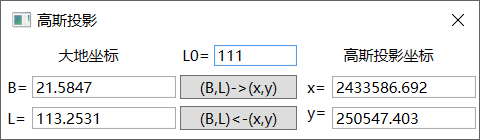
\includegraphics[scale=1]{chapter/gaussProj/UI01.png}
    \caption{简单的高斯投影正反算界面}
    \label{fig:GaussProjUI01}
\end{figure}

相应的主要界面代码如下:

\begin{lstlisting}[language=xml]
<TextBlock Text="大地坐标" HorizontalAlignment="Center"
        VerticalAlignment="Center"/>
<TextBlock  Text="B=" Grid.Row="1" Margin="5"/>
<TextBox x:Name="textBox_B" Grid.Row="1"
        Text=""
        VerticalAlignment="Center"  Margin="25,0,0,0"/>
<TextBlock  Text="L=" Margin="5" Grid.Row="2" />
<TextBox x:Name="textBox_L"
        Text=""
        VerticalAlignment="Center" Margin="25,0,0,0" Grid.Row="2" />

<TextBlock  Text="L0=" Grid.Column="1"
        Margin="5,0,0,0" VerticalAlignment="Center"/>
<TextBox x:Name="textBox_L0"
        Text=""
        Grid.Column="1"
        Margin="30,0,3,0" VerticalAlignment="Center"/>
<Button Content="(B,L)->(x,y)" Grid.Column="1" Grid.Row="1"
                Click="BLtoXYButton_Click" Margin="3,3"/>
<Button Content="(B,L)&lt;-(x,y)" Grid.Column="1" Grid.Row="2"
                Click="XYtoBLButton_Click"  Margin="3,3"/>
        
<TextBlock Text="高斯投影坐标" Grid.Column="2"
                HorizontalAlignment="Center" VerticalAlignment="Center"/>
<TextBlock  Text="x=" Margin="5" Grid.Row="1" Grid.Column="2"/>
<TextBox x:Name="textBox_x" Grid.Row="1" Grid.Column="2"
                Text=""
                Margin="25,0,0,0" VerticalAlignment="Center" />
<TextBlock Text="y=" Grid.Row="2" Grid.Column="2" Margin="5,0,0,0"/>
<TextBox x:Name="textBox_y"
                Text=""
                Grid.Row="2"  Grid.Column="2"
                Margin="25,0,0,0" VerticalAlignment="Center" />       
\end{lstlisting}

请注意,在这段xaml界面代码中,由于我们的算法需要与界面上的TextBox控件进行数据交换,
每个TextBox都需要命名(如上的每个TextBox控件都有一个 x:Name 属性)。

相应的正算与反算按钮响应事件代码如下:

\begin{lstlisting}
private void BLtoXYButton_Click(object sender, RoutedEventArgs e)
{
    double B, L, L0, x, y;
    double.TryParse(this.textBox_B.Text, out B);
    double.TryParse(this.textBox_L.Text, out L);
    double.TryParse(this.textBox_L0.Text, out L0);

    Spheroid proj = Spheroid.CreateBeiJing1954();
    proj.BLtoXY(
        ZXY.SMath.DMS2RAD(B),
        ZXY.SMath.DMS2RAD(L),
        ZXY.SMath.DMS2RAD(L0),
        out x, out y);
    this.textBox_x.Text = x.ToString();
    this.textBox_y.Text = y.ToString();
}

private void XYtoBLButton_Click(object sender, RoutedEventArgs e)
{
    double B, L, L0, x, y;
    double.TryParse(this.textBox_x.Text, out x);
    double.TryParse(this.textBox_y.Text, out y);
    double.TryParse(this.textBox_L0.Text, out L0);

    Spheroid proj = Spheroid.CreateBeiJing1954();
    proj.XYtoBL(x, y,
        ZXY.SMath.DMS2RAD(L0),
        out B, out L);
    this.textBox_B.Text =ZXY.SMath.RAD2DMS(B).ToString();
    this.textBox_L.Text = ZXY.SMath.RAD2DMS(L).ToString();
}
\end{lstlisting}

在这个两个响应事件中,首先需要直接从界面上的TextBox控件中取值,
由于TextBox的Text属性是文本(string类型),需要用double.TryParse
函数将其转换为double类型。

其次我们默认参考椭球为1954北京坐标系的参考椭球,需要将其创建,此处我们用
类的静态函数可以方便创建,不必记忆其椭球的几何参数值。

然后我们就可以调用我们前边写的正算与反算函数进行高斯投影正反算了,算完后
将值再赋值给相应的TextBox控件的Text属性就可以了。注意传入函数的值如果是度分秒形式的角度,
应该先调用我们前边的写的函数将其转换为弧度,如果算出的值也是角度,也应该调用我们
前面所写的函数将其转换为度分秒形式。


\subsection{界面程序的优化}
上面的简单界面程序存在着一个很大的问题,就是从界面取数据时无法判断数据的有效性等,
也无法发挥WPF界面技术。WPF界面技术里的数据绑定功能(binding)可以很好的简化这一过程。

我们仔细分析前边的界面,这个程序的实质就是一个点的两种形式的坐标之间的转换,
因此我们可以定义一个点类GeoPoint,其定义如下:

\begin{lstlisting}
public class GeoPoint
{
    public string Name { get; set;} //点名
    public double B { get; set;}    //纬度,单位:度分秒
    public double L { get; set;}    //经度,单位:度分秒
    public double L0 { get; set;}   //中央子午线经度,单位:度分秒
    public double X { get; set;}    //X坐标
    public double Y { get; set;}    //Y坐标
}
\end{lstlisting}

则在界面代码中可对TextBox的Text做如下绑定:

\begin{lstlisting}
<TextBlock Text="大地坐标" HorizontalAlignment="Center"
        VerticalAlignment="Center"/>
<TextBlock  Text="B=" Grid.Row="1" Margin="5"/>
<TextBox x:Name="textBox_B" Grid.Row="1"
        Text="{Binding B}"
        VerticalAlignment="Center"  Margin="25,0,0,0"/>
<TextBlock  Text="L=" Margin="5" Grid.Row="2" />
<TextBox x:Name="textBox_L"
        Text="{Binding L}"
        VerticalAlignment="Center" Margin="25,0,0,0" Grid.Row="2" />

<TextBlock  Text="L0=" Grid.Column="1"
        Margin="5,0,0,0" VerticalAlignment="Center"/>
<TextBox x:Name="textBox_L0"
        Text="{Binding L0}" 
        Grid.Column="1"
        Margin="30,0,3,0" VerticalAlignment="Center"/>
<Button Content="(B,L)->(x,y)" Grid.Column="1" Grid.Row="1"
        Click="BLtoXYButton_Click" Margin="3,3"/>
<Button Content="(B,L)&lt;-(x,y)" Grid.Column="1" Grid.Row="2"
        Click="XYtoBLButton_Click"  Margin="3,3"/>
        
<TextBlock Text="高斯投影坐标" Grid.Column="2"
        HorizontalAlignment="Center" VerticalAlignment="Center"/>
<TextBlock  Text="x=" Margin="5" Grid.Row="1" Grid.Column="2"/>
<TextBox x:Name="textBox_x" Grid.Row="1" Grid.Column="2"
        Text="{Binding X}"
        Margin="25,0,0,0" VerticalAlignment="Center" />
<TextBlock Text="y=" Grid.Row="2" Grid.Column="2" Margin="5,0,0,0"/>
<TextBox x:Name="textBox_y"
        Text="{Binding Y}"
        Grid.Row="2"  Grid.Column="2"
        Margin="25,0,0,0" VerticalAlignment="Center" />  
\end{lstlisting}

以上代码中的TextBox控件中的x:Name属性甚至都可以省略。由于这些控件都是
以这个窗体(Window)作为容器的,他们的数据源都可用这个窗体的DataContext
一次性设置,让系统以冒泡的形式自动为属性绑定寻找数据源。窗体为之
设定数据源的代码如下:

\begin{lstlisting}
public partial class MainWindow : Window
{
    private GeoPoint geoPoint;
    private Spheroid proj = Spheroid.CreateBeiJing1954();

    public MainWindow()
    {
        InitializeComponent();
        geoPoint = new GeoPoint(){ B= 21.58470845, L= 113.25314880 };
        this.DataContext = geoPoint;
    }
    //.......省略了其他代码......
}
\end{lstlisting}

程序中由于正反算都是基于相同的椭球基准,所以在类MainWindow中定义了
geoPoint实例字段与proj实例字段。在构造函数中为其赋了初值以简化每次在
界面输入数据,为这个窗体的DataContext指定点的各项属性绑定的数据源。

相应的正反算按钮的响应事件修改为:

\begin{lstlisting}
private void BLtoXYButton_Click(object sender, RoutedEventArgs e)
{
    double x, y;
    proj.BLtoXY(
        ZXY.SMath.DMS2RAD(geoPoint.B),
        ZXY.SMath.DMS2RAD(geoPoint.L),
        ZXY.SMath.DMS2RAD(geoPoint.L0),
        out x, out y);
    geoPoint.X = x; geoPoint.Y = y;
}

private void XYtoBLButton_Click(object sender, RoutedEventArgs e)
{
    double B, L;
    proj.XYtoBL(geoPoint.X, geoPoint.Y,
       ZXY.SMath.DMS2RAD(geoPoint.L0),
       out B, out L);
    geoPoint.B = ZXY.SMath.RAD2DMS(B);
    geoPoint.L = ZXY.SMath.RAD2DMS(L);
}
\end{lstlisting}

从响应事件可以看出,代码简洁了很多。运行程序时,TextBox框中都有默认数值,
而且非数值数据也输入不进去了,也不需要将文本框中的Text属性转换为double类型了。
一切看似都好,但你发现在点击正算或反算按钮时,界面上的数据没有变化,好像功能没有实现一样,
问题出现在什么地方呢?

我们回过头再看GeoPoint的定义,发现其属性定义过于简单。根据WPF知识可知,在对象属性发生改变时
(如我们的计算中正算改变了X与Y,反算改变了B与L),还需要一种机制通知系统需要刷新界面,
这就需要类GeoPoint从接口 INotifyPropertyChanged 继承并实现它
(该接口所在的命名空间为System.ComponentModel)。修改后的GeoPoint类如下:

\begin{lstlisting}
public class GeoPoint : INotifyPropertyChanged
{
    public event PropertyChangedEventHandler PropertyChanged;

    public void RaisePropertyChange(string propertyName)
    {
        if (this.PropertyChanged != null)
        {
            this.PropertyChanged.Invoke(this, 
                new PropertyChangedEventArgs(propertyName));
        }
    }

    private string _name;
    public string Name //点名
    {
        get { return _name; }
        set
        {
            _name = value;
            RaisePropertyChange("Name");
        }
    }

    private double _B;
    public double B //纬度,单位:度分秒
    {
        get { return _B; }
        set
        {
            _B = value;
            RaisePropertyChange("B");
        }
    }

    private double _L;
    public double L //经度,单位:度分秒
    {
        get { return _L; }
        set
        {
            _L = value;
            RaisePropertyChange("L");
        }
    }

    private double _L0;
    public double L0 //中央子午线经度,单位:度分秒
    {
        get { return _L0; }
        set
        {
            _L0 = value;
            RaisePropertyChange("L0");
        }
    }

    private double _X;
    public double X //X坐标
    {
        get { return _X; }
        set
        {
            _X = value;
            RaisePropertyChange("X");
        }
    }
  
    private double _Y;
    public double Y  //Y坐标
    {
        get { return _Y; }
        set
        {
            _Y = value;
            RaisePropertyChange("Y");
        }
    }
}
\end{lstlisting}

与前面的GeoPoint类相比较,现在的这个类从 INotifyPropertyChanged 继承
并实现了接口成员PropertyChanged,在属性值发生改变时利用该接口成员通知界面
属性值发生了变化。

运行程序,功能一切正常。


\subsection{点类的进一步优化}

我们再次审阅界面程序后的正反算代码,发现事实上的正反算都是基于点类的,
也就是说只与GeoPoint类相关,因此我们将正反算功能移到GeoPoint类中,
以进一步简化界面的方法调用。其代码如下:

\begin{lstlisting}
public class GeoPoint : INotifyPropertyChanged
{
    //......其它代码.......
    public void BLtoXY(Spheroid spheroid)
    {
        double x, y;
        spheroid.BLtoXY(
           ZXY.SMath.DMS2RAD(this.B),
           ZXY.SMath.DMS2RAD(this.L),
           ZXY.SMath.DMS2RAD(this.L0),
           out x, out y);
        this.X = x; this.Y = y;
    }

    public void XYtoBL(Spheroid spheroid)
    {
        double B, L;
        spheroid.XYtoBL(X, Y, ZXY.SMath.DMS2RAD(this.L0),
           out B, out L);
        this.B = ZXY.SMath.RAD2DMS(B);
        this.L = ZXY.SMath.RAD2DMS(L);
    }
}
\end{lstlisting}

界面正反算代码可以进一步简化为如下形式:

\begin{lstlisting}
private void BLtoXYButton_Click(object sender, RoutedEventArgs e)
{
    geoPoint.BLtoXY(proj);
}

private void XYtoBLButton_Click(object sender, RoutedEventArgs e)
{
    geoPoint.XYtoBL(proj) ;
}
\end{lstlisting}

至此,我们的算法与界面几乎是完全分离了,这符合我们第一章所讲的界面与算法相
分离的原则,也为我们的算法进行单元测试和进一步优化迭代打下了基础。


\section{更加实用的多点计算图形程序}

上面的程序从编程的角度讲比较完美了,但从实用的角度来说还有很多缺点,
比如不能选择椭球基准,不能进行多点的正反算,不能读取和写出文本文件数据。
这一节我们将从算法和界面两个方面来构造这个更加实用的多点高斯投影计算的
图形程序。

\subsection{程序的功能}

实用的高斯投影程序功能如下:

\begin{enumerate}
\item 椭球基准的选择:能够自由的选择参考椭球基准,或者自定义参考椭球;
\item 能实现高斯投影正反算与换带功能;
\item 高斯投影坐标的定义:能自动去除或添加点的Y坐标前的常数500km和带号;
\item 数据的界面录入:能利用程序界面组织输入数据;
\item 能导入导出文本数据:能将外部文本数据导入到程序中,能将程序中的数据导出为文本文件;
\item 能实现多个点的批量计算。
\end{enumerate}

软件运行时的界面如图\ref{fig:GaussProjUI02}所示,该界面基本能满足以上功能。

\begin{figure}[htbp]
    \centering
    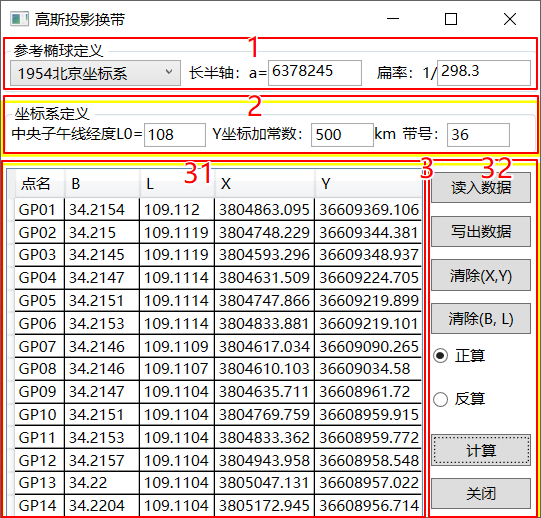
\includegraphics[scale=1]{chapter/gaussProj/UI02.png}
    \caption{实用高斯投影程序界面}
    \label{fig:GaussProjUI02}
\end{figure}

\subsection{程序的面向对象分析与实现}

从界面上我们可以看出,程序中应该包含三部分内容:
椭球基准、坐标系、点集。为了满足以上功能,我们需要对我们的程序进行重构。

分析我们前边的 GeoPoint 类会发现,一个点有中央子午线经度 L0 这个属性会很奇怪,
而在实际应用中点集也是基于坐标系的点集,一个点集的y坐标甚至x坐标前的加常数也是基本相同。
因此坐标系应该有中央子午线经度 L0属性,带号N与Y坐标前的加常数YKM,
由于坐标系是依赖于椭球基准的,也应有椭球基准属性ProjSpheroid。
坐标系类的定义如下代码所示:

\begin{lstlisting}
using System.Collections.ObjectModel;

/// <summary>
/// 坐标系
/// </summary>
public class CoordinateSystem : INotifyPropertyChanged
{
    //....省略与接口INotifyPropertyChanged有关的代码....

    /// <summary>
    /// 中央子午线经度
    /// </summary>
    private double _L0;
    
    /// <summary>
    /// 中央子午线经度
    /// </summary>
    public double L0
    {
        get { return _L0; }
        set
        {
            _L0 = value;
            RaisePropertyChange("L0");
        }
    }
    
    /// <summary>
    /// 带号
    /// </summary>
    private int _N;
    
    /// <summary>
    /// 带号
    /// </summary>
    public int N
    {
        get { return _N; }
        set
        {
            _N = value;
            RaisePropertyChange("N");
        }
    }
    
    /// <summary>
    /// Y坐标的加常数
    /// </summary>
    private double _YKM;
    
    /// <summary>
    /// Y坐标的加常数
    /// </summary>
    public double YKM
    {
        get { return _YKM; }
        set
        {
            _YKM = value;
            RaisePropertyChange("YKM");
        }
    }
    
    /// <summary>
    /// 坐标点集
    /// </summary>
    private ObservableCollection<GeoPoint>geoPointList = 
        new ObservableCollection<GeoPoint>();
    
    /// <summary>
    /// 坐标点集
    /// </summary>
    public ObservableCollection<GeoPoint> GeoPointList
    {
        get { return geoPointList; }
    }
    
    /// <summary>
    /// 投影椭球基准
    /// </summary>
    private Spheroid spheroid = Spheroid.CreateBeiJing1954();
    
    /// <summary>
    /// 投影椭球基准
    /// </summary>
    public Spheroid ProjSpheroid
    {
        get { return spheroid; }
        set
        {
            spheroid = value;
            RaisePropertyChange("ProjSpheroid");
        }
    }

   public CoordinateSystem(){ }
}
\end{lstlisting}

在类GeoPoint中将属性L0的定义删除。在CoordinateSystem类中,由于
N,L0,YKM需与界面交互,故须从接口 INotifyPropertyChanged 继承。

为与WPF界面中的DataGrid控件交互,点集需要用ObservableCollection<GPoint> 表达,
不能用List<GPoint>,而且默认状态下就应该生成其实例对象。注意二者的命名空间也不一样,
前者为System.Collections.ObjectModel,
用于界面交互较多,后者为 System.Collections.Generic,用于不需要界面的
算法较多。

为了与界面的初始状态一致,对投影的参考椭球我们默认生成北京54坐标系的
参考椭球。

在我们的程序中GeoPoint类与CoordinateSystem类为了处理与界面交互的
问题,都需要实现接口 INotifyPropertyChanged,实现接口的代码重复。
本着相同或相似的代码在程序中只写一次的原则,我们将这部分的代码独立到
类 NotificationObject 中,让GeoPoint类与CoordinateSystem类从
NotificationObject 类继承。相应的实现代码如下:

\begin{lstlisting}
using System.ComponentModel;

namespace GaussProj
{
    public class NotificationObject : INotifyPropertyChanged
    {
        public event PropertyChangedEventHandler PropertyChanged;

        public void RaisePropertyChange(string propertyName)
        {
            if (this.PropertyChanged != null)
            {
                this.PropertyChanged.Invoke(this, new PropertyChangedEventArgs(propertyName));
            }
        }
    }
}

public class GeoPoint : NotificationObject
{
    //删除与NotificationObject类中相同的代码
    //省略GeoPoint类中的内容
}

public class CoordinateSystem : NotificationObject
{
    //删除与NotificationObject类中相同的代码
    //省略CoordinateSystem类中的内容
}
\end{lstlisting}

\subsection{多点的高斯投影计算}

如此,在类CoordinateSystem中就有了用于高斯投影的椭球基准,
有了坐标系的中央子午线经度,有了带号及y坐标前的加常数与点集,
多点的高斯投影计算就万事俱备,只欠实现了。其实现代码如下:

\begin{lstlisting}
public class CoordinateSystem : NotificationObject 
{
    //省略其他代码

    /// <summary>
    /// 多点高斯投影正算
    /// </summary>
    public void BLtoXY()
    {
        foreach (var pnt in this.geoPointList)
        {
            pnt.BLtoXY(spheroid, this);
        }
    }

    /// <summary>
    /// 多点高斯投影反算
    /// </summary>
    public void XYtoBL()
    {
        foreach (var pnt in this.geoPointList)
        {
            pnt.XYtoBL(spheroid, this);
        }
    }
}
\end{lstlisting}

从代码中可以看出,在类CoordinateSystem中并没有真正的进行高斯投影正算与
反算,而是通过循环将其委托给每个点的实例了。

点类GeoPoint中的高斯投影正反算实现如下:

\begin{lstlisting}
public class GeoPoint : NotificationObject
{
    //省略其他代码
    /// <summary>
    /// 高斯投影正算
    /// </summary>
    /// <param name="spheroid">投影椭球</param>
    /// <param name="cs">坐标系</param>
    public void BLtoXY(Spheroid spheroid, CoordinateSystem cs)
    {
        double x, y;
        spheroid.BLtoXY(
           ZXY.SMath.DMS2RAD(this.B),
           ZXY.SMath.DMS2RAD(this.L),
           ZXY.SMath.DMS2RAD(cs.L0),
           out x, out y);
        this.X = x; this.Y = y + cs.YKM * 1000 + cs.N * 1000000;
    }
    /// <summary>
    /// 高斯投影反算
    /// </summary>
    /// <param name="spheroid">投影椭球</param>
    /// <param name="cs">坐标系</param>
    public void XYtoBL(Spheroid spheroid, CoordinateSystem cs)
    {
        double tB, tL;
        double y = Y - cs.YKM * 1000 - cs.N * 1000000;
        spheroid.XYtoBL(X, y, ZXY.SMath.DMS2RAD(cs.L0),
           out tB, out tL);
        this.B = ZXY.SMath.RAD2DMS(tB);
        this.L = ZXY.SMath.RAD2DMS(tL);
    }
}
\end{lstlisting}

从如上的代码中可以看出,真正的高斯投影正反算还是在我们前面写的Spheroid类中。
请注意在Spheroid类中,所有的与角度有关的单位是弧度,y坐标也是点的真实坐标,
在此我们需要根据坐标系中的信息对其做相应的预处理。

还应注意,在BLtoXY中,为了与界面交互,要赋值给this.X与this.Y,而不是赋值给其变量
this.\_X与this.\_Y。在 XYtoBL 中也同样如此,当然还需要将计算出的弧度值转换为度分秒形式。

\subsection{点坐标数据的读入与写出}

利用我们的界面可以手工输入点的坐标数据,但导入与导出文本数据对于一个
程序来讲是必不可少的功能。

为了避免我们的教学程序过于复杂,我们对数据文件的格式进行适当简化。

在高斯投影正算时,所需的数据应该是:点名,纬度B, 经度L,设计我们的文本文件
内容如下:

\begin{verbatim}
 #点名,   B,   L
GP01,34.2154,109.112
GP02,34.215,109.1119
GP03,34.2145,109.1119
GP04,34.2147,109.1114
GP05,34.2151,109.1114
\end{verbatim}

文件中的每一行第一个字符以 \#开头的我们视为注释行,予以忽略。

在高斯投影反算时,所需的数据应该是:点名,X, Y,设计我们的文本文件
内容如下:

\begin{verbatim}
#点名,       X,       Y,         H
GP01, 3805709.2106, 19333388.3123, 466.419
GP02, 3805595.1034, 19333360.1973, 470.94
GP03, 3805440.0738, 19333360.1727, 478.728
GP04, 3805481.9494, 19333237.0999, 475.975
GP05, 3805598.4201, 19333235.7343, 469.738
\end{verbatim}

文件中的数据项可以多余三项,我们只读取第1、2、3项,其余忽略。

在写出数据时,我们将点的五项数据:点名,B, L, X, Y 全部写出,
如下所示:

\begin{verbatim}
# 点名,    B,      L,     X,      Y 
GP01, 34.2154, 109.112  , 3804863.095, 36609369.106
GP02, 34.215,   109.1119, 3804748.229, 36609344.381
GP03, 34.2145, 109.1119, 3804593.296, 36609348.937
GP04, 34.2147, 109.1114, 3804631.509, 36609224.705
GP05, 34.2151, 109.1114, 3804747.866, 36609219.899
\end{verbatim}

用户在使用时可以将其数据拷贝到Word中按分隔符 ``,''生成表格进行编辑
处理,或按分隔符 ``,''导入到Excel中进行编辑排版处理。

读入的点坐标数据应存储在我们的程序中,很显然应该在类CoordinateSystem中
实现读入文本文件数据功能,写出数据的功能也如此,其实现代码如下:

\begin{lstlisting}
public class CoordinateSystem : NotificationObject 
{
    //省略其他代码

    /// <summary>
    /// 读入点集坐标数据
    /// </summary>
    /// <param name="fileName">文件名</param>
    /// <param name="format">点的坐标格式:BL-Name,B,L  
    ///                                 XY-Name,X,Y
    /// </param>
    public void ReadGeoPointData(string fileName, string format)
    {
        using (System.IO.StreamReader sr = new System.IO.StreamReader(fileName) )
        {
            string buffer;
            //读入点的坐标数据
            this.GeoPointList.Clear();
            while (true)
            {
                buffer = sr.ReadLine();
                if (string.IsNullOrEmpty(buffer)) break; //文件末尾或空行退出
                if (buffer[0] == '#') continue;
                string[] its = buffer.Split(new char[1] { ',' });
                if (its.Length < 3) continue; //少于三项数据,不是点的坐标数据,忽略
                GeoPoint pnt = new GeoPoint();
                pnt.Name = its[0].Trim(); 
                if (format == "XY")
                {                       
                    pnt.X = double.Parse(its[1]); 
                    pnt.Y = double.Parse(its[2]);
                    pnt.B = 0; pnt.L = 0;
                }
                else if (format == "BL")
                {
                    pnt.B = double.Parse(its[1]); 
                    pnt.L = double.Parse(its[2]); 
                    pnt.X = 0; pnt.Y = 0;
                }
               
                this.GeoPointList.Add(pnt);
            }
        }
    }

    /// <summary>
    /// 写出点集坐标数据
    /// </summary>
    /// <param name="fileName">文件名</param>
    public void WriteGeoPointData(string fileName)
    {
        using (System.IO.StreamWriter sr = new System.IO.StreamWriter(fileName))
        {
            sr.WriteLine("#点名,   B,   L,  X,  Y");
            foreach (var pnt in this.geoPointList)
            {
                sr.WriteLine( pnt );
            }
        }
    }
}
\end{lstlisting}

写数据比较简单,按要求写出即可,需要注意的是第57行,在函数WriteLine中
我们直接写出了GeoPoint的实例对象pnt,这需要在GeoPoint中将ToString()
进行override,实现代码如下:
\begin{lstlisting}
public class GeoPoint : NotificationObject
{
    public override string ToString()
    {
        return string.Format("{0},{1:0.0000},{2:0.0000},{3:0.000},{4:0.000}", Name, B, L, X, Y);
    }
}
\end{lstlisting}

在占位符中我们加入了输出浮点数据的格式控制,保证输出的角度小数位数不超过四位,
输出的坐标不超过三位。

读入数据相对于写出数据要由于需要解码数据,所以要复杂一些。小于三个数据项
的行我们直接略过,同时我们能加入格式控制,如果格式控制BL,
意味着数据文件是经纬度数据,其他属性相应置零。

读入数据的这段代码我们实现的方式较为粗略,只是通过逗号分隔的数据项个数
进行了判断,这在真正的程序开发中是不可靠的,可以通过正则表达式对每行数据进行检验,
对符合要求的文本数据加以处理,以此来提高读取文本数据功能的容错能力。

清除(X, Y)与清除(B, L)功能实质上是将点的这些属性置零,比较简单,相应代码如下:

\begin{lstlisting}
public class CoordinateSystem : NotificationObject 
{
    //省略其他代码

    public void ClearXY()
    {
        foreach (var pnt in this.geoPointList)
        {
            pnt.X = pnt.Y = 0;
        }
    }
    public void ClearBL()
    {
        foreach (var pnt in this.geoPointList)
        {
            pnt.B = pnt.L = 0;
        }
    }
}
\end{lstlisting}


\subsection{界面设计与实现}

按图\ref{fig:GaussProjUI02}设计的界面代码如下:

\begin{lstlisting}[language=xml]
<Window x:Class="GaussProj.GaussProjWin"
        xmlns="http://schemas.microsoft.com/winfx/2006/xaml/presentation"
        xmlns:x="http://schemas.microsoft.com/winfx/2006/xaml"
        xmlns:d="http://schemas.microsoft.com/expression/blend/2008"
        xmlns:mc="http://schemas.openxmlformats.org/markup-compatibility/2006"
        xmlns:local="clr-namespace:GaussProj"
        mc:Ignorable="d"
        Title="高斯投影换带" Height="360" Width="540">
    <Grid>
        <Grid.RowDefinitions>
            <RowDefinition Height="45"/>
            <RowDefinition Height="5"/>
            <RowDefinition Height="45"/>
            <RowDefinition Height="5"/>
            <RowDefinition Height="Auto"/>
        </Grid.RowDefinitions>
        <GroupBox x:Name="groupBox_spheroid" Header="参考椭球定义" 
            DataContext="ProjSpheroid" Margin="1">
            <Grid>
                <Grid.ColumnDefinitions>
                    <ColumnDefinition Width="200*"/>
                    <ColumnDefinition Width="70"/>
                    <ColumnDefinition Width="110*"/>
                    <ColumnDefinition Width="60"/>
                    <ColumnDefinition Width="110*"/>
                </Grid.ColumnDefinitions>
                <ComboBox Grid.Column="0" x:Name="comboBox_Spheroid" 
                          SelectionChanged="comboBox_Spheroid_SelectionChanged">
                    <ComboBoxItem  Content="1954北京坐标系" Tag="BJ1954"/>
                    <ComboBoxItem Content="1980西安坐标系" Tag="XA1980"/>
                    <ComboBoxItem Content="CGCS2000大地坐标系" Tag="CGCS2000"/>
                    <ComboBoxItem Content="自定义参考椭球" Tag="CS0000"/>
                </ComboBox>
                <TextBlock Text="长半轴:a=" Grid.Column="1" 
                    VerticalAlignment="Center" HorizontalAlignment="Right"/>
                <TextBox x:Name="textBox_a" Grid.Column="2" Text="{Binding a}"/>
                <TextBlock Text="扁率:1/" Grid.Column="3" 
                    VerticalAlignment="Center" HorizontalAlignment="Right"/>
                <TextBox x:Name="textBox_f" Grid.Column="4" Text="{Binding f}"/>
            </Grid>
        </GroupBox>

        <Border  Grid.Row="2" BorderBrush="Yellow" BorderThickness="2">
            <GroupBox x:Name="groupBox_CoordinateSystem" Header="坐标系定义">
            <StackPanel Orientation="Horizontal">
                <TextBlock Text="中央子午线经度L0=" />
                <TextBox x:Name="textBox_L0" Text="{Binding L0}" Width="50"/>
                <TextBlock Text="Y坐标加常数:" Margin="5,0,0,0" />
                <TextBox x:Name="textBox_YKM" Text="{Binding YKM}" Width="50"/>
                <TextBlock Text="km" />
                <TextBlock Text="带号:" Margin="5,0,0,0"/>
                <TextBox x:Name="textBox_N" Text="{Binding N}" Width="50"/>
            </StackPanel>
            </GroupBox>
        </Border>
        
        <Border  Grid.Row="4" BorderBrush="Yellow" BorderThickness="2">
            <Grid>
                <Grid.ColumnDefinitions>
                    <ColumnDefinition Width="200*"/>
                    <ColumnDefinition Width="90"/>
                </Grid.ColumnDefinitions>
                <DataGrid x:Name="dataGrid_ctrPnt" 
                    AutoGenerateColumns="False" Margin="2" 
                    ItemsSource="{Binding GeoPointList}" >
                <DataGrid.Columns>
                    <DataGridTextColumn Header="点名" 
                        Binding="{Binding Name}"
                        MinWidth="40"/>
                    <DataGridTextColumn Header="B" 
                        Binding="{Binding B , StringFormat={}{0:##0.####}}" 
                        MinWidth="60"/>
                    <DataGridTextColumn Header="L" 
                        Binding="{Binding L , StringFormat={}{0:##0.####}}" 
                        MinWidth="60"/>
                    <DataGridTextColumn Header="X" 
                        Binding="{Binding X , StringFormat={}{0:##0.###}}" 
                        MinWidth="60"/>
                    <DataGridTextColumn Header="Y" 
                        Binding="{Binding Y, StringFormat={}{0:##0.###}}"
                        MinWidth="60" />
                </DataGrid.Columns>
            </DataGrid>

                <StackPanel Grid.Column="1" Orientation="Vertical">
                    <RadioButton x:Name="radioButton_BLtoXY"  Content="正算" 
                        Height="25" Width="80" Margin="5"/>
                    <RadioButton x:Name="radioButton_XYtoBL"  Content="反算" 
                        IsChecked="True" Height="25" Width="80" Margin="5" />

                    <Button x:Name="Button_ReadGaussProjData" Content="读入数据"
                        Height="25" Width="80" Margin="5" 
                        Click="Button_ReadGaussProjData_Click"/>
                    <Button x:Name="Button_WriteGaussProjData" Content="写出数据" 
                        Height="25" Width="80" Margin="5" 
                        Click="Button_WriteGaussProjData_Click"/>

                    <Button x:Name="Button_ClearXY" Content="清除(X,Y)" 
                        Height="25" Width="80" Margin="5" 
                        Click="Button_ClearXY_Click"/>
                    <Button x:Name="Button_ClearBL" Content="清除(B, L)" 
                        Height="25" Width="80" Margin="5" 
                        Click="Button_ClearBL_Click"/>
                    
                    <Button x:Name="Button_CalGaussProj"  Content="计算" 
                        Height="25" Width="80" Margin="5" 
                        Click="Button_CalGaussProj_Click"/>
                    <Button x:Name="Button_Close" Content="关闭" 
                        Height="25" Width="80" Margin="5" 
                        Click="Button_Close_Click"/>
                </StackPanel>
            </Grid>
        </Border>     
    </Grid>
</Window>
\end{lstlisting}

在这段xaml代码中,除了功能按钮区外,实际上分为了三部分:

第一部分为参考椭球定义,如第18行代码所示,我们将其布局到
 groupBox\_spheroid中,数据绑定a与f,数据源设置在groupBox\_spheroid中,
 采用冒泡搜寻类CoordinateSystem中的ProjSpheroid属性。

为了简化示例程序的编写,ComboBox中的参考椭球类型采用硬编码方式直接写在其中了。
通过SelectionChange事件对不同的椭球类型选择进行响应。

第二部分为坐标系定义,同样采用数据绑定的形式与界面交互数据,数据源来自
类CoordinateSystem。

第三部分为点集部分,数据源为类CoordinateSystem中的GeoPointList属性,如
第65行代码所示。

界面后台代码如下:

\begin{lstlisting}
public partial class GaussProjWin : Window
{       
    private CoordinateSystem myCoordinateSystem;

    public GaussProjWin()
    {
        InitializeComponent();

        myCoordinateSystem = new CoordinateSystem() {
            L0 = 111, N = 19, YKM = 500};
        this.DataContext = myCoordinateSystem;

        this.comboBox_Spheroid.SelectedIndex = 0;
    }

    //省略其他代码
}
\end{lstlisting}

在窗体后台代码中,我们设置了窗体类的类实例变量myCoordinateSystem完成
各项功能。在其窗体类的构造函数中实例化并对其属性赋了初始值,同时将
窗体的DataContex属性设为myCoordinateSystem,完成数据绑定的数据源设置。
同时为了维持与界面属性的一致性,将comboBox\_Spheroid的SelectedIndex设为0。

界面的其它功能按钮的实现比较简单,实现代码如下:

\begin{lstlisting}
public partial class GaussProjWin : Window
{   
    //省略其他代码

    private void comboBox_Spheroid_SelectionChanged(object sender, 
        SelectionChangedEventArgs e)
    {
        if(comboBox_Spheroid.SelectedIndex == 0)
            myCoordinateSystem.ProjSpheroid = Spheroid.CreateBeiJing1954();
        else if (comboBox_Spheroid.SelectedIndex == 1)
            myCoordinateSystem.ProjSpheroid = Spheroid.CreateXian1980();
        else if (comboBox_Spheroid.SelectedIndex == 2)
            myCoordinateSystem.ProjSpheroid = Spheroid.CreateCGCS2000();
        else if (comboBox_Spheroid.SelectedIndex == 3)
            myCoordinateSystem.ProjSpheroid = 
                Spheroid.CreateCoordinateSystem(6378137, 298.257222101);
        this.groupBox_spheroid.DataContext = myCoordinateSystem.ProjSpheroid;
    }

    private void Button_ReadGaussProjData_Click(object sender,
        RoutedEventArgs e)
    {
        OpenFileDialog dlg = new OpenFileDialog();
        dlg.DefaultExt = ".txt";
        dlg.Filter = "高斯投影坐标数据|*.txt|All File(*.*)|*.*";
        if (dlg.ShowDialog() != true) return;

        if (this.radioButton_BLtoXY.IsChecked == true)
            myCoordinateSystem.ReadGeoPointData(dlg.FileName, "BL");
        else if(this.radioButton_XYtoBL.IsChecked == true)
            myCoordinateSystem.ReadGeoPointData(dlg.FileName, "XY");
    }

    private void Button_WriteGaussProjData_Click(object sender, 
        RoutedEventArgs e)
    {
        SaveFileDialog dlg = new SaveFileDialog();
        dlg.DefaultExt = ".txt";
        dlg.Filter = "高斯投影坐标数据|*.txt|All File(*.*)|*.*";
        if (dlg.ShowDialog() != true) return;

        myCoordinateSystem.WriteGeoPointData(dlg.FileName);
    }

    private void Button_ClearXY_Click(object sender, RoutedEventArgs e)
    {
        myCoordinateSystem.ClearXY();
    }

    private void Button_ClearBL_Click(object sender, RoutedEventArgs e)
    {
        myCoordinateSystem.ClearBL();
    }

    private void Button_CalGaussProj_Click(object sender, RoutedEventArgs e)
    {
        if (radioButton_BLtoXY.IsChecked == true)
            myCoordinateSystem.BLtoXY();
        else if (radioButton_XYtoBL.IsChecked == true)
            myCoordinateSystem.XYtoBL();
    }

    private void Button_Close_Click(object sender, RoutedEventArgs e)
    {
        this.Close();
    }
}
\end{lstlisting}

\subsection{换带功能的实现}

在我们以上的设计中好像没有换带计算,虽然没有直接实现,但确实是实现了。
在前边的论述中,我们讲过,换带计算的实质是变换坐标系的中央子午线位置,
过程为:先进行坐标反算,然后变换中央子午线经度,再反算新的坐标即可。

\begin{figure}[htbp]
    \centering
    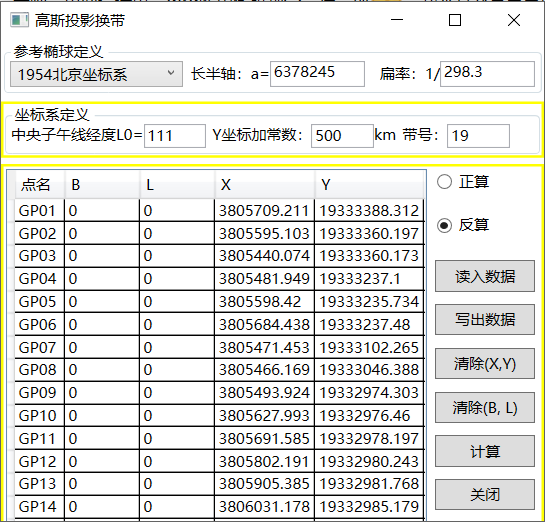
\includegraphics[scale=0.8]{chapter/gaussProj/UI03.png}
    \caption{$6\degree$带第19带数据界面}
    \label{fig:GaussProjUI03}
\end{figure}

启动程序,在反算的模式下读入数据,如图\ref{fig:GaussProjUI03}所示,这是一6度带第
19带的北京54坐标:

点击计算,反算各点的大地坐标经纬度,如图\ref{fig:GaussProjUI04}所示。

\begin{figure}[htbp]
    \centering
    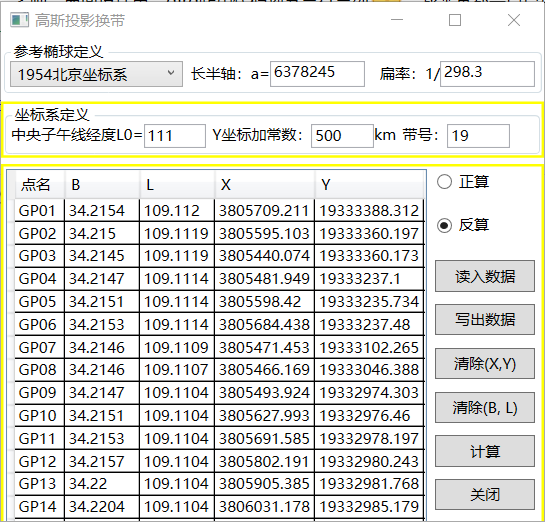
\includegraphics[scale=0.8]{chapter/gaussProj/UI04.png}
    \caption{$6\degree$带第19带反算数据界面}
    \label{fig:GaussProjUI04}
\end{figure}

现在我们准备将其换带到3度带的38带坐标系去,设置中央子午线经度L0为108,
带号设为36,选择正算,点击清除(x,y)按钮将X,Y坐标设置为0,如图\ref{fig:GaussProjUI05}所示:

\begin{figure}[htbp]
    \centering
    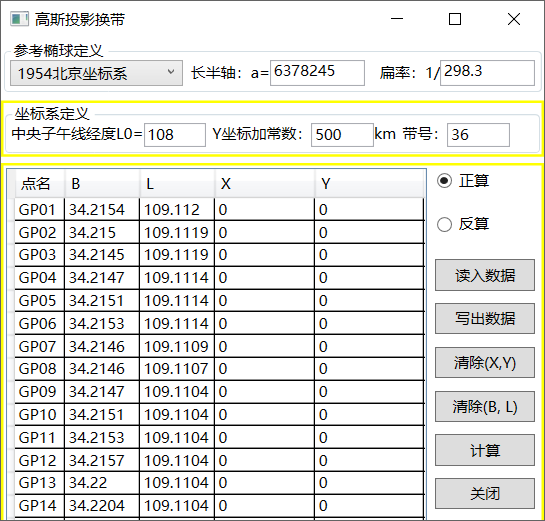
\includegraphics[scale=0.8]{chapter/gaussProj/UI05.png}
    \caption{设置$3\degree$带第36带数据界面}
    \label{fig:GaussProjUI05}
\end{figure}

点击计算按钮,计算出新坐标系下各点的坐标,如图\ref{fig:GaussProjUI06}所示:
\begin{figure}[htbp]
    \centering
    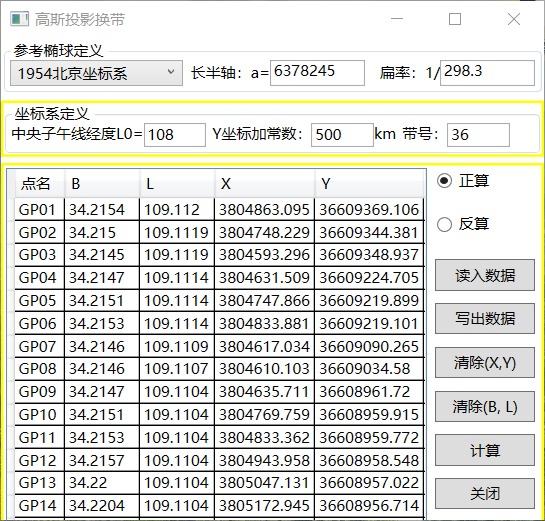
\includegraphics[scale=0.8]{chapter/gaussProj/UI06.png}
    \caption{$3\degree$带第36带正算数据界面}
    \label{fig:GaussProjUI06}
\end{figure}

到此就完成了换带功能,可以点击写出数据按钮将计算成果输出。

\section{扩展}

\subsection{UTM投影}

北半球: $x = x_r + 0$

南半球: $x = x_r + 10,000,000$, 加一万公里

Y坐标: $y = y_r + 500,000$, 加五百公里

需要注意的是:

UTM投影的分带与国际1:100万地图的划分一致,从 $180\degree$起向东每$6\degree$为一带。
因此, 高斯-克吕格投影的第一带($0\degree - 6\degree E$)为UTM投影的第31带,
UTM投影的第一带($180\degree - 174\degree W$)为高斯-克吕格投影的第31带.

\subsection{注意事项}

以上过程也可以看成是我们这个软件的教程。但应注意,换带计算只限于相同椭球
基准的情况才能应用,不能在不同椭球基准间应该该功能。

以上换带功能也可以设计一个界面,在新的界面上将新旧坐标系的中央子午线经度
都设置出,从而完成一键式换带计算功能。

\subsection{空间直角坐标系与大地坐标之间的转换}

随着我国对CGCS2000大地坐标系的推广应用与北斗导航系统的日益成熟,将大地坐标 $(B, L, H)$
与空间直角坐标 $(X, Y, Z)$ 进行相互转换的应用也会越来越多。如果能实现大地坐标 $(B, L, H)$
与空间直角坐标 $(X, Y, Z)$ 的相互转换,也就可以实现空间直角坐标 $(X, Y, Z)$
到高斯平面坐标的投影计算了,进而在桌面端电脑或移动设备上编程实现更多的功能应用。

大地坐标 $(B, L, H)$ 与空间直角坐标 $(X, Y, Z)$ 的相互转换公式如下:

已知大地坐标计算空间直角坐标的公式:
\begin{equation}
\left .
\begin{aligned}
X &= (N+H) \cos B \cos L \\
Y &= (N+H) \cos B \sin L \\
Z &= [N(1 - e^2) + H)] \sin B 
\end{aligned} 
\right \}
\end{equation}

已知空间直角坐标$(X,Y,Z)$计算大地坐标$(B, L, H)$的公式如下:

\begin{equation}
\left . 
\begin{aligned}
L &= \arctan \frac{Y}{X} \\
\tan B &= \frac{Z + Ne^2 \sin B}{\sqrt{X^2 + Y^2}} \\
H &= \frac{Z}{sinB} - N(1-e^2)  \\
 or  \\
H &=\frac{\sqrt{X^2 + Y^2}}{\cos B} - N 
\end{aligned} 
\right \}
\end{equation}

由以上公式可以看出,L 可以直接由X,Y算出,B 则需要迭代计算。

可对上面公式的B直接进行迭代计算,其过程如下:

% \begin{equation}
%     B = \arctan { \frac{Z+Ne^2 \sin B}{\sqrt{X^2 + Y^2}}}
% \end{equation}

先取B的初始值为:$B_0 =\arctan{ (Z / \sqrt{X^2 + Y^2} ) }$ 计算出$N$与$\sin B_0$,
代入上式,计算出新的B值$B_1$。然后将新的$B_1$代入再计算,直到两次的B值满足所要求的
精度。

或将:
$$N = \frac{c}{\sqrt{1+e'^2 \cos ^2 B}}$$
与$$\frac{1}{\cos^2 B} = 1+ \tan^2 B$$

代入到上式中,得到:
\begin{equation}
    \tan B = \frac{Z}{\sqrt{X^2 + Y^2}} + \frac{ce^2 \cdot \tan B}{\sqrt{X^2 + Y^2} \cdot \sqrt{1 + e'^2 + \tan^2 B}}
\end{equation}

则可令 $tB = \tan B$,对公式两边的 tB 进行迭代计算,当满足精度要求时,再求出B值 $B = \arctan (tB)$ 即可。 %% 没有\atan 这个函数

本处只是列出了基本的计算公式与计算思路,大家可以查找资料寻找更加高效的计算方法予以实现。

\subsection{同基准下的椭球膨胀法}

我们经常在一些资料中见到椭球膨胀法建立独立坐标系或施工坐标系的方法,
椭球膨胀法是依据某种给定的参考椭球,根据测区的平均高程和平距纬度将
椭球面扩大而维持扁率不变,也可以应用换带的方法将椭球膨胀后的坐标与原坐标系的
坐标进行相互转换。但应注意椭球膨胀后,各个点的纬度值也会发生变化,
在这种换带过程中需要修正各个点的纬度值,大家可以参看这方面的资料。


平距曲率半径:

$$R_m = \sqrt{MN}= a \frac{\sqrt{1-e^2}}{1-e^2 \sin^2 B_m}$$


子午曲率半径

$$
\left .
\begin{aligned}
M &= \frac{a \cdot (1-e^2)}{\sqrt{(1-e^2 \sin ^2 B)^3}} \\
N &= \frac{a}{\sqrt{1-e^2 \sin^2 B}}
\end{aligned} 
\right \}
$$


用 $R_m$ 求 a

$$a = \frac{1-e^2 \sin^2 B_m }{\sqrt{1-e^2}} R_m$$


新椭球的平均曲率半径 $R'_m$
$$R'_m = R_m + H_m = a \frac{\sqrt{1-e^2}}{1-e^2 \sin^2 B_m} + H_m$$

则有:
$$da = \frac{1-e^2 \sin ^2 B_m}{\sqrt{1-e^2}} \cdot H_m$$

由于是同基准的椭球膨胀,所以公式中的平移量$\Delta X_0, \Delta Y_0, \Delta Z_0$ 均为0,
旋转量$\varepsilon_X, \varepsilon_Y, \varepsilon_Z$ 均为0,尺度变化参数$m=0$, 扁率变化参数$\Delta \alpha=0$。公式(2-77)可以简化为:


$$
\left .
\begin{aligned}
dL &= 0 \\
dB &= \frac{N}{(M+H) \cdot a} e^2 \sin B \cos B \cdot \Delta a  \\
dH &= -\frac{N}{a}(1-e^2 \sin ^2 B ) \cdot \Delta a
\end{aligned} 
\right \}
$$


\section*{小结}

我们从较为简单的单点高斯投影正反算程序开始,运用
 \cs 知识与WPF界面技术实现了一个较为实用的高斯投影正反算与换带
程序。

在程序过程中,我们遵循了界面与算法相分离的原则,运用了WPF的
事件绑定等技术。

这个程序从功能上讲还是有许多不足的,从易用性上也还有许多值得改进的
地方。希望随着我们的 \cs 知识与WPF技术的积累,能在以后将它优化得更好!


                   %%高斯投影程序设计


%!TEX root = ../../clcxsj.tex

\chapter{平面坐标系统之间的转换}

在某些工程中,由于不知道新旧两种坐标系的建立方法或参数,因此无法用换带计算的方法
进行坐标转换。如果知道某些点在两个坐标系中的坐标值,我们就可以采用一些近似的转换方
法将其它的点也转换到新坐标系中,求出其坐标值。尤其对于较低等级的大量控制点来说,
采用这些近似方法,能够快速得到转换结果。

 \section{原理和数学模型}

\subsection{原理}
这些方法的实质是根据新旧网的重合点(又称为公共点)的坐标值之差,按一定的规律修正
旧网的各点坐标值,使旧网最恰当的配合到新网内。修正时因不合观测值改正数平方和为最
小的原则,故为近似方法。

\begin{figure}[htbp]
    \centering
    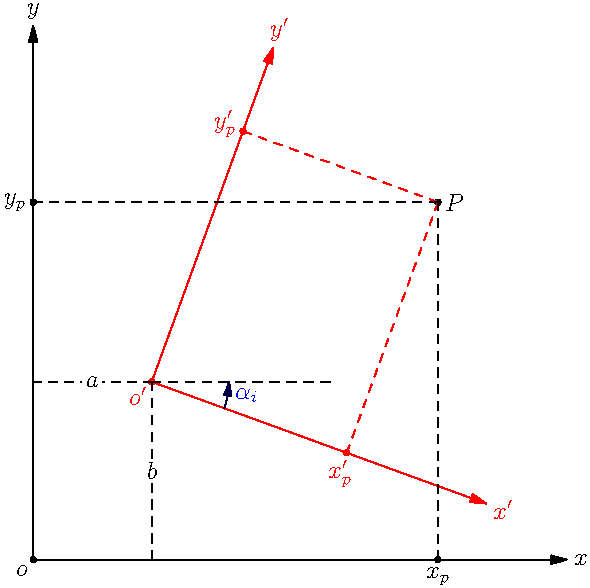
\includegraphics[scale=1]{chapter/xytoxy/xytoxy.pdf}
    \caption{坐标相似变换示意图}
    \label{fig:xytoxy}
\end{figure}

常用的方法有简单变换方法(又称赫尔默特法或相似变换法)、仿射变换法、正形变换法等。
在这里我们主要讲解简单变换法。

\subsection{相似变换法的数学模型}
实质是使旧网坐标系平移、旋转和进行尺度因子改正,将旧网配合到新网上。因旧网形状保
持不变,故称为平面相似变换法。

变换方程为:
$$\left.
\begin{array}{l}
\textrm{$x=a+k(x'\cos\alpha+y'\sin\alpha)$} \\
\textrm{$y=b+k(-x'\sin\alpha+y'\cos\alpha)$}
\end{array}\right\}$$

式中$a$,$b$表示平移,$\alpha$是旧网$x'$轴逆转至新网$x$轴的转角,$k$为尺度因子。
这些变换参数是未知的,要根据新旧网公共点上的已知坐标$x$,$y$和$x'$、$y'$求解确定。

因此必须至少有两个公共点,列出四个方程式,解算出这四个未知参数值。如果具有两个以
上的公共点时,就应该应用最小二乘平差方法,求解最或是参数值。

为解算出这些参数,我们引入参数$c$、$d$:

$c=k\cos\alpha$,$d=k\sin\alpha$

将公式转换为:
$$\left.
\begin{array}{l}
\textrm{$x=a+x'c+y'd$}\\
\textrm{$y=b+y'c-x'd¥$}
\end{array}\right\}$$

由于新旧网都存在测量误差,设新旧坐标$x$,$y$和$x'$,$y'$的误差分别为
$v_x$,$v_y$和$v_{x'}$,$v_{y'}$,因此上式改写为:

$$\left.\begin{array}{l}
\textrm{$x+v_x=a+(x'+v_{x'})c+(y'+v_{y'})d$} \\
\textrm{$y+v_y=b+(y'+v_{y'})c-(x'+v_{x'})d$}
\end{array}\right\}$$

设:
$$\left.\begin{array}{l}
\textrm{$n_x=-v_x+cv_{x'}+dv_{y'}$} \\
\textrm{$n_y=-v_y-dv_{x'}+cv_{y'}$}
\end{array}\right\}$$

则有:
$$\left.\begin{array}{l}
\textrm{$-n_x=a+x'c+y'd-x$} \\
\textrm{$-n_y=b+y'c-x'd-y$}
\end{array}\right\}$$

若有$r$个新旧网的公共点,则可组成$r$对方程:
$$V=BX-l$$

上式即为参数平差时的方程,$l$代表观测向量,$V$代表改正数向量,$B$代表系数矩阵,
$X$是参数向量。它们的值为:

$\mathbf{V}=
\left(\begin{array}{c}
-n_{x1} \\ -n_{y1} \\ \vdots \\ -n_{xr} \\ -n_{yr}
\end{array}\right)$
$\mathbf{B}=
\left(\begin{array}{cccc}
1 & 0 & x'_1 & y'_1 \\
0 & 1 & y'_1 & -x'_1 \\
\dots & \dots & \ldots & \ldots \\
1 & 0 & x'_r & y'_r \\
0 & 1 & y'_r & -x'_r
\end{array}\right)$
$\mathbf{X}=
\left(\begin{array}{c}
a \\ b \\ c \\ d
\end{array}\right)$
$\mathbf{l}=
\left(\begin{array}{c}
x_1 \\ y_1 \\ \vdots \\ x_r \\ y_r
\end{array}\right)$

根据最小二乘原理$V^TV=min$可得到法方程:
$$B^TBX-B^Tl=0$$

解法方程可求得$a$、$b$、$c$、$d$的值:
$$X=(B^TB)^{-1}(B^Tl)$$

旋转角$\alpha$和尺度比$k$为:
$$\alpha=\arctan\frac{d}{c}$$
$$k=\sqrt{c^2+d^2}$$
之后,就可计算旧网中所有待转换点的新坐标。

请注意,以上图及公式推导是按数学坐标系进行的,在用测量坐标代入计算时
应将测量坐标$(x,y)$以$(y,x)$形式代入,否则应对以上图形与公式进行变换。

\section{程序设计与实现}

程序整体功能比较单一,从数学模型分析可看出,程序的关
键是在于如何组成系数矩阵$B$与常数项$l$。

\subsection{程序功能分析}

在程序中,我们需要能够有录入数据界面手工输入数据,能够导入与导出
文本文件形式组织的数据,能够输出计算成果,能够计算转换系数或根据已有的
转换系数也能计算待计算点在新坐标系中的坐标。

由此,我们设计出程序界面如图\ref{fig:XYtoXYUI02}所示:

\begin{figure}[htbp]
    \centering
    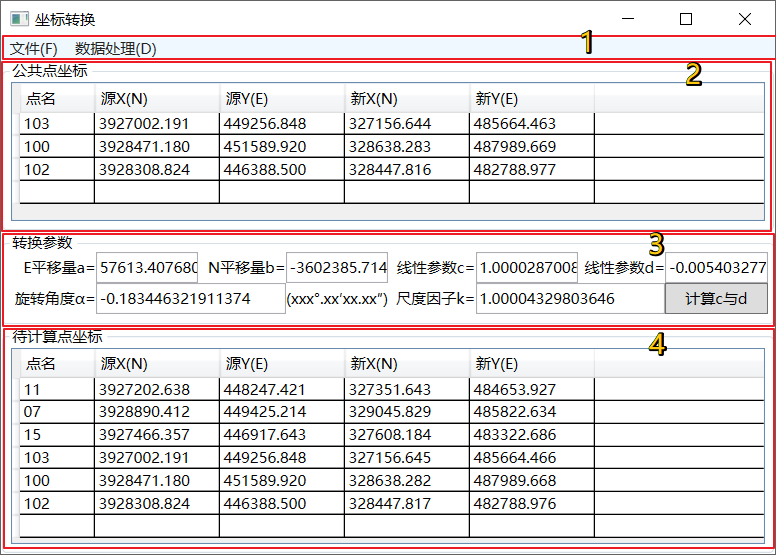
\includegraphics[scale=1]{chapter/xytoxy/XYtoXYUI02.png}
    \caption{坐标转换程序界面}
    \label{fig:XYtoXYUI02}
\end{figure}

\subsection{程序界面设计}

由图\ref{fig:XYtoXYUI02}分析可知,界面分为菜单、公共点坐标、转换参数与
待计算点坐标四个部分。

整个界面采用DockPanel布局,以加入菜单项,使用菜单项进行功能计算可以有效节省
界面的布局空间。余下的部分采用Grid布局,将其划分为三行,
即三个部分。第一行中加入GroupBox控件作为标题,在其中加入DataGrid控件;
第二部分中加入Grid布局,将其二行八列进行布局;第三部分同第一部分一样。

由于需要根据输入的a、b、$\alpha$、k计算各点在新坐标系中的坐标,为了输入
旋转角度的便捷性(直接输入度分秒),因此加入了计算c与d的按钮。程序中计算各待计算点坐标
时实际使用的参数是$a,b,c,d$。

整个界面布局xaml代码如下:
\begin{lstlisting}[language=xml]
<DockPanel LastChildFill="True">
        <Menu  x:Name="mainmenu" DockPanel.Dock="Top" Background="AliceBlue">
            <MenuItem Header="文件(F)">
                <MenuItem Header="打开文本数据"
                    Click="menuItem_OpenTextFileData_Click"/>
                <MenuItem Header="保存文本数据"
                    Click="menuItem_SaveTextFileData_Click"/>
                <Separator/>
                <MenuItem Header="退出" Click="menuItem_Exit_Click"/>
            </MenuItem>
            <MenuItem Header="数据处理(D)">
                <MenuItem Header="计算转换参数" 
                    Click="menuItem_CalCoefficient_Click" />
                <MenuItem Header="计算待计算点坐标" 
                    Click="menuItem_Cal_UnKnw_XY_Click" />
                <Separator/>
                <MenuItem Header="写出计算成果" 
                    Click="menuItem_Write_Result_Click" />
            </MenuItem>
        </Menu>

        <Grid>
            <Grid.RowDefinitions>
                <RowDefinition Height="150*"/>
                <RowDefinition Height="75"/>
                <RowDefinition Height="200*"/>
            </Grid.RowDefinitions>
            <GroupBox Header="公共点坐标" Grid.Row="0">
                <DataGrid AutoGenerateColumns="False" Margin="2" 
                    ItemsSource="{Binding KnwPointList}">
                    <DataGrid.Columns>
                        <DataGridTextColumn Header="点名" MinWidth="60"
                            Binding="{Binding Name}"  />
                        <DataGridTextColumn Header="源X(N)" MinWidth="100"
                            Binding="{Binding OX, StringFormat={}{0:0.000}}"/>
                        <DataGridTextColumn Header="源Y(E)" MinWidth="100"
                            Binding="{Binding OY, StringFormat={}{0:0.000}}"/>
                        <DataGridTextColumn Header="新X(N)"  MinWidth="100"
                            Binding="{Binding NX, StringFormat={}{0:0.000}}"/>
                        <DataGridTextColumn Header="新Y(E)" MinWidth="100"
                            Binding="{Binding NY, StringFormat={}{0:0.000}}"/>
                    </DataGrid.Columns>
                </DataGrid>
            </GroupBox>

            <GroupBox Header="转换参数" Grid.Row="1">
                <Grid>
                    <Grid.ColumnDefinitions>
                        <ColumnDefinition Width="70"/>
                        <ColumnDefinition Width="120*"/>
                        <ColumnDefinition Width="70"/>
                        <ColumnDefinition Width="120*"/>
                        <ColumnDefinition Width="70"/>
                        <ColumnDefinition Width="120*"/>
                        <ColumnDefinition Width="70"/>
                        <ColumnDefinition Width="120*"/>
                    </Grid.ColumnDefinitions>
                    <Grid.RowDefinitions>
                        <RowDefinition Height="25"/>
                        <RowDefinition Height="25"/>
                    </Grid.RowDefinitions>
                    <TextBlock Text="E平移量a=" Grid.Row="0" Grid.Column="0" 
                        VerticalAlignment="Center" HorizontalAlignment="Right"/>
                    <TextBox x:Name="textBox_a" Grid.Row="0" Grid.Column="1" 
                        Text="{Binding a}" 
                        VerticalContentAlignment="Center"/>
                    <TextBlock Text="N平移量b=" Grid.Row="0" Grid.Column="2"  
                        VerticalAlignment="Center" HorizontalAlignment="Right"/>
                    <TextBox x:Name="textBox_b" Grid.Row="0" Grid.Column="3"  
                        Text="{Binding b}"
                        VerticalContentAlignment="Center"/>
                    <TextBlock Text="线性参数c=" Grid.Row="0" Grid.Column="4" 
                        VerticalAlignment="Center" HorizontalAlignment="Right"/>
                    <TextBox x:Name="textBox_c" Grid.Row="0" Grid.Column="5" 
                        Text="{Binding c}"
                        VerticalContentAlignment="Center"/>
                    <TextBlock Text="线性参数d=" Grid.Row="0" Grid.Column="6" 
                        VerticalAlignment="Center" HorizontalAlignment="Right"/>
                    <TextBox x:Name="textBox_d" Grid.Row="0" Grid.Column="7"  
                        Text="{Binding d}" 
                        VerticalContentAlignment="Center"/>
                    <TextBlock Text="旋转角度α=" Grid.Row="1" Grid.Column="0" 
                        VerticalAlignment="Center" HorizontalAlignment="Right"/>
                    <TextBox x:Name="textBox_alpha" Grid.Row="1" Grid.Column="1"  
                        Text="{Binding alpha}" 
                        Grid.ColumnSpan="2"
                        VerticalContentAlignment="Center"/>
                    <TextBlock Text="(xxx°.xx′xx.xx″)" Grid.Row="1" Grid.Column="3" 
                        VerticalAlignment="Center" HorizontalAlignment="Right"/>
                    <TextBlock Text="尺度因子k=" Grid.Row="1" Grid.Column="4" 
                        VerticalAlignment="Center" HorizontalAlignment="Right"/>
                    <TextBox x:Name="textBox_k" Grid.Row="1" Grid.Column="5" 
                        Text="{Binding k}" 
                        Grid.ColumnSpan="2"
                        VerticalContentAlignment="Center"/>
                    <Button x:Name="button_Cal_cd"  Content="计算c与d"
                        Grid.Row="1" Grid.Column="7" 
                        Click="button_Cal_cd_Click"/>
                </Grid>
            </GroupBox>

            <GroupBox Header="待计算点坐标" Grid.Row="2">
                <DataGrid AutoGenerateColumns="False" Margin="2" 
                    ItemsSource="{Binding UnKnwPointList}">
                    <DataGrid.Columns>
                        <DataGridTextColumn Header="点名" MinWidth="60"
                            Binding="{Binding Name}"  />
                        <DataGridTextColumn Header="源X(N)"  MinWidth="100"
                            Binding="{Binding OX, StringFormat={}{0:0.000}}"/>
                        <DataGridTextColumn Header="源Y(E)" MinWidth="100"
                            Binding="{Binding OY, StringFormat={}{0:0.000}}"/>
                        <DataGridTextColumn Header="新X(N)" MinWidth="100"
                            Binding="{Binding NX,StringFormat={}{0:0.000}}" />
                        <DataGridTextColumn Header="新Y(E)" MinWidth="100"
                            Binding="{Binding NY, StringFormat={}{0:0.000}}" />
                    </DataGrid.Columns>
                </DataGrid>
            </GroupBox>
        </Grid>
    </DockPanel>
\end{lstlisting}

\subsection{数据文件和成果文件格式}
由于程序的功能较为单一,数据文件的格式也较为简单。我们设计格式如下:
\begin{verbatim}
#赫尔默特四参数转换法数据文件
#每行以“#”开头的行均被认为是注释行
#公共点在源坐标系中的坐标: 点名, X(N), Y(E)
103, 3927002.191, 449256.848
100, 3928471.180, 451589.920
102, 3928308.824, 446388.500

#公共点在目标坐标系中的坐标: 点名, X(N), Y(E)
102, 328447.816, 482788.977
103, 327156.644, 485664.463
100, 328638.283, 487989.669

#待转换点在源坐标系中的坐标: 点名, X(N), Y(E)
11,   3927202.638, 448247.421
07,   3928890.412, 449425.214
15,   3927466.357, 446917.643
103, 3927002.191, 449256.848
100, 3928471.180, 451589.920
102, 3928308.824, 446388.500
\end{verbatim}

我们设计成果文件的格式如下:

\begin{verbatim}
#赫尔默特四参数转换法计算成果数据文件
# 公共点坐标
# 点名, 源X(N), 源Y(E), 新X(N), 新Y(E)
103,3927002.191,449256.848,327156.644,485664.463
100,3928471.180,451589.920,328638.283,487989.669
102,3928308.824,446388.500,328447.816,482788.977

# 转换参数
a=57613.4076806228,b=-3602385.71435623, c=1.00002870085641, d=-0.00540327780963763
α=-0.183446321911374,k=1.00004329803646

# 待计算点的坐标
# 点名, 源X(N), 源Y(E), 新X(N), 新Y(E)
11,3927202.638,448247.421,327351.643,484653.927
07,3928890.412,449425.214,329045.829,485822.634
15,3927466.357,446917.643,327608.184,483322.686
103,3927002.191,449256.848,327156.645,485664.466
100,3928471.180,451589.920,328638.282,487989.668
102,3928308.824,446388.500,328447.817,482788.976
\end{verbatim}

\subsection{程序流程}
根据以上分析,程序流程如下:
\begin{enumerate}
  \item 读取公共点旧坐标
  \item 读取公共点新坐标
  \item 组成误差方程式
  \item 解算参数向量
  \item 解算待定点的坐标
  \item 将计算成果写入文件
\end{enumerate}


\subsection{主要功能设计}
为了实现以上功能,我们需要设计一个类(或结构)用于表示点,设计如下:
\begin{lstlisting}[language=C]
namespace CoordniateTransform
{
    public class GeoPoint : NotificationObject
    {
        private string _name;
        public string Name //点名
        {
            get { return _name; }
            set
            {
                _name = value;
                RaisePropertyChange("Name");
            }
        }       

        private double _oX;
        public double OX //源X坐标
        {
            get { return _oX; }
            set
            {
                _oX = value;
                RaisePropertyChange("OX");
            }
        }
  
        private double _oY;
        public double OY  //源Y坐标
        {
            get { return _oY; }
            set
            {
                _oY = value;
                RaisePropertyChange("OY");
            }
        }


        private double _nX;
        public double NX //新X坐标
        {
            get { return _nX; }
            set
            {
                _nX = value;
                RaisePropertyChange("NX");
            }
        }

        private double _nY;
        public double NY  //新Y坐标
        {
            get { return _nY; }
            set
            {
                _nY = value;
                RaisePropertyChange("NY");
            }
        }

 
        public override string ToString()
        {
            return string.Format("{0},{1:0.000},{2:0.000},{3:0.000},{4:0.000}", Name, OX, OY, NX, NY);
        }
    }
}
\end{lstlisting}

类NotificationObject的设计见前一章内容。


同时,我们设计另一个类CoordinateSystem来完成相应的其它功能, 这个类相当于一个容器一样,
它包括点集(已知公共点集和待计算点集)、转换参数等,具体代码如下:

\begin{lstlisting}[language=C]
using System;
using System.Collections.ObjectModel;

namespace CoordniateTransform
{
    /// <summary>
    /// 坐标系
    /// </summary>
    public class CoordinateSystem : NotificationObject
    {
        /// <summary>
        /// 公共点集
        /// </summary>
        private ObservableCollection<GeoPoint> knwPointList = 
                new ObservableCollection<GeoPoint>();

        /// <summary>
        /// 公共点集
        /// </summary>
        public ObservableCollection<GeoPoint> KnwPointList
        {
            get { return knwPointList; }
        }
        
        /// <summary>
        /// 待计算点集
        /// </summary>
        private ObservableCollection<GeoPoint> unKnwPointList = 
                new ObservableCollection<GeoPoint>();

        /// <summary>
        ///待计算点集
        /// </summary>
        public ObservableCollection<GeoPoint> UnKnwPointList
        {
            get { return unKnwPointList; }
        }

        /// <summary>
        ///X方向平移量
        /// </summary>
        private double _a;

        /// <summary>
        /// X方向平移量
        /// </summary>
        public double a
        {
            get { return _a; }
            set
            {
                _a = value;
                RaisePropertyChange("a");
            }
        }

        /// <summary>
        /// Y方向平移量
        /// </summary>
        private double _b;

        /// <summary>
        /// Y方向平移量
        /// </summary>
        public double b
        {
            get { return _b; }
            set
            {
                _b = value;
                RaisePropertyChange("b");
            }
        }

        /// <summary>
        /// 线性方程计算系数c
        /// </summary>
        public double _c;

        /// <summary>
        /// 线性方程计算系数c
        /// </summary>
        public double c
        {
            get { return _c; }
            set
            {
                _c = value;
                RaisePropertyChange("c");
            }
        }

        /// <summary>
        /// 线性方程计算系数d
        /// </summary>
        public double _d;

        /// <summary>
        /// 线性方程计算系数d
        /// </summary>
        public double d
        {
            get { return _d; }
            set
            {
                _d = value;
                RaisePropertyChange("d");
            }
        }

        /// <summary>
        /// 旋转角度α
        /// </summary>
        public double _alpha;

        /// <summary>
        ///  旋转角度α
        /// </summary>
        public double alpha
        {
            get { return _alpha; }
            set
            {
                _alpha = value;
                RaisePropertyChange("alpha");
            }
        }

        /// <summary>
        /// 尺度比因子k
        /// </summary>
        public double _k;

        /// <summary>
        ///  尺度比因子k
        /// </summary>
        public double k
        {
            get { return _k; }
            set
            {
                _k = value;
                RaisePropertyChange("k");
            }
        }

        public CoordinateSystem(){ }

        /// <summary>
        /// 读入坐标转换数据文件
        /// </summary>
        /// <param name="fileName">文件名</param>
        public void ReadTextFileData(string fileName)
        {
            using (System.IO.StreamReader sr = new System.IO.StreamReader(fileName))
            {
                string buffer;

                //读入点的坐标数据
                this.KnwPointList.Clear();
                while (true)//读入公共点源坐标系坐标数据,至空行退出
                {
                    buffer = sr.ReadLine();
                    if (string.IsNullOrEmpty(buffer)) break; //文件末尾或空行退出

                    if (buffer[0] == '#') continue;

                    string[] its = buffer.Split(new char[1] { ',' });
                    if (its.Length == 3)
                    {
                        GeoPoint pnt = new GeoPoint();
                        pnt.Name = its[0].Trim();
                        pnt.OX = double.Parse(its[1]);
                        pnt.OY = double.Parse(its[2]);
                        this.KnwPointList.Add(pnt);
                    }
                }

                while (true)//读入公共点新坐标系坐标数据,至空行退出
                {
                    buffer = sr.ReadLine();
                    if (string.IsNullOrEmpty(buffer)) break; //文件末尾或空行退出

                    if (buffer[0] == '#') continue;

                    string[] its = buffer.Split(new char[1] { ',' });
                    if (its.Length == 3)
                    {
                        string name = its[0].Trim();
                        GeoPoint pnt = GetGeoPoint(name);
                        pnt.NX = double.Parse(its[1]);
                        pnt.NY = double.Parse(its[2]);
                    }
                }

                this.UnKnwPointList.Clear();
                while (true)//读入待计算点源坐标系坐标数据,至空行退出
                {
                    buffer = sr.ReadLine();
                    if (string.IsNullOrEmpty(buffer)) break; //文件末尾或空行退出

                    if (buffer[0] == '#') continue;

                    string[] its = buffer.Split(new char[1] { ',' });
                    if (its.Length == 3)
                    {
                        GeoPoint pnt = new GeoPoint();
                        pnt.Name = its[0].Trim();
                        pnt.OX = double.Parse(its[1]);
                        pnt.OY = double.Parse(its[2]);

                        this.UnKnwPointList.Add(pnt);
                    }
                }
            }
        }
     
        /// <summary>
        /// 根据点名获取点对象
        /// </summary>
        /// <param name="name">点名</param>
        /// <returns>点对象</returns>
        private GeoPoint GetGeoPoint(string name)
        {
            foreach (var it in this.KnwPointList)
            {
                if (it.Name == name)
                    return it;
            }

            return null;
        }

        /// <summary>
        /// 写坐标转换数据文件
        /// </summary>
        /// <param name="fileName">文件名</param>
        public void WriteTextFileData(string fileName)
        {
            using (System.IO.StreamWriter sr = new System.IO.StreamWriter(fileName))
            {
                sr.WriteLine("#赫尔默特四参数转换法数据文件");
                sr.WriteLine("#每行以“#”开头的行均被认为是注释行");
                sr.WriteLine("#公共点在源坐标系中的坐标: 点名, X(N), Y(E)");
                foreach (var pnt in this.knwPointList)
                {
                    sr.WriteLine("{0}, {1}, {2}", pnt.Name, pnt.OX, pnt.OY);
                }

                sr.WriteLine();
                sr.WriteLine("#公共点在新坐标系中的坐标: 点名, X(N), Y(E)");
                foreach (var pnt in this.knwPointList)
                {
                    sr.WriteLine("{0}, {1}, {2}", pnt.Name, pnt.NX, pnt.NY);
                }

                sr.WriteLine();
                sr.WriteLine("#待转换点在源坐标系中的坐标: 点名, X(N), Y(E)");
                foreach (var pnt in this.unKnwPointList)
                {
                    sr.WriteLine("{0}, {1}, {2}", pnt.Name, pnt.OX, pnt.OY);
                }
            }
        }
        /// <summary>
        /// 写计算成果数据文件
        /// </summary>
        /// <param name="fileName">文件名</param>
        public void WriteResultTextFileData(string fileName)
        {
            using (System.IO.StreamWriter sr = new System.IO.StreamWriter(fileName))
            {
                sr.WriteLine("#赫尔默特四参数转换法计算成果数据文件");
                sr.WriteLine("# 公共点坐标");
                sr.WriteLine("# 点名, 源X(N), 源Y(E), 新X(N), 新Y(E)");
                foreach (var pnt in this.knwPointList)
                {
                    sr.WriteLine(pnt);
                }

                sr.WriteLine();
                sr.WriteLine("# 转换参数");
                sr.WriteLine("a={0},b={1}, c={2}, d={3}\r\nα={4},k={5}", 
                    this.a, this.b, this.c, this.d, this.alpha, this.k);

                sr.WriteLine();
                sr.WriteLine("# 待计算点的坐标");
                sr.WriteLine("# 点名, 源X(N), 源Y(E), 新X(N), 新Y(E)");
                foreach (var pnt in this.unKnwPointList)
                {
                    sr.WriteLine(pnt);
                }
            }
        }

        /// <summary>
        /// 根据尺度比因子d与旋转角度α计算线性计算量c和d
        /// </summary>
        public void CalCd()
        {
            this.c = this.k * Math.Cos(ZXY.SMath.DMS2RAD(this.alpha));
            this.d = this.k * Math.Sin(ZXY.SMath.DMS2RAD(this.alpha));
        }

        /// <summary>
        /// 赫尔默特法计算转换系数
        /// </summary>
        public void CalCoefficient()
        {
            int n0 = this.knwPointList.Count;
            if (n0 < 2) return; //少于两个公共点,无法计算

            double[,] B = new double[2 * n0, 4];
            double[] l = new double[2 * n0];
            double[,] N = new double[4, 4];
            double[] U = new double[4];

            //组成系数阵B与l,此处应注意读入的坐标是测量坐标,
            //应将测量坐标转换为数学坐标
            double x, y, xT, yT;
            for (int i = 0; i < n0; i++)
            {
                x = knwPointList[i].OY;//数学上的x,测量上的y
                y = knwPointList[i].OX;//数学上的y,测量上的x
                xT = knwPointList[i].NY;
                yT = knwPointList[i].NX; 

                B[(2 * i), 0] = 1.0;
                B[(2 * i), 1] = 0.0;
                B[(2 * i), 2] = x;
                B[(2 * i), 3] = y;
                l[2 * i] = xT;

                B[(2 * i + 1), 0] = 0.0;
                B[(2 * i + 1), 1] = 1.0;
                B[(2 * i + 1), 2] = y; 
                B[(2 * i + 1), 3] = -x; 
                l[2 * i + 1] = yT;
            }

            for (int k = 0; k < 4; k++)
            {
                for (int j = 0; j < 4; j++)
                {
                    N[k, j] = 0.0;
                    for (int i = 0; i < 2 * n0; i++)
                    {
                        N[k, j] += B[i, k] * B[i, j];
                    }
                }

                U[k] = 0.0;
                for (int i = 0; i < 2 * n0; i++)
                    U[k] += B[i, k] * l[i];
            }

            NegativeMatrix(N, U, 4);

            this.a = U[0];
            this.b = U[1];
            this.c = U[2];
            this.d = U[3];
            this.alpha = ZXY.SMath.RAD2DMS(Math.Atan2(d, c));
            this.k = Math.Sqrt(d * d + c * c);
        }

        /// <summary>
        /// 计算点在新坐标系中的坐标
        /// </summary>
        public void CalUnKnwXY()
        {
            //应将测量坐标转换为数学坐标
            double x, y, xT, yT;
            foreach (var it in this.unKnwPointList)
            {
                x = it.OY; y = it.OX;

                xT = this.a + this.c * x + this.d * y;
                yT = this.b + this.c * y - this.d * x;

                it.NY = xT; it.NX = yT;
            }
        }

        /// <summary>
        ///  高斯约化法解方程 AX = B中的X值, 结果存B中
        /// </summary>
        /// <param name="A">A: nxn</param>
        /// <param name="B">B: nx1</param>
        /// <param name="n">n</param>
        private void NegativeMatrix(double[,] A, double[] B, int n)
        {
            for (int k = 0; k < n - 1; k++)
            {
                for (int i = k + 1; i < n; i++)
                {
                    A[i, k] /= A[k, k];
                    for (int j = k + 1; j < n; j++)
                    {
                        A[i, j] -= A[i, k] * A[k, j];
                    }
                    B[i] -= A[i, k] * B[k];
                }
            }
            B[n - 1] /= A[(n - 1), (n - 1)];
            for (int i = n - 2; i >= 0; i--)
            {
                double s = 0.0;
                for (int j = i + 1; j < n; j++)
                {
                    s += A[i, j] * B[j];
                }
                B[i] = (B[i] - s) / A[i, i];
            }
        }
    }
}
\end{lstlisting}

界面响应代码如下:

\begin{lstlisting}[language=C]
using Microsoft.Win32;
using System;
using System.Collections.Generic;
using System.Linq;
using System.Text;
using System.Threading.Tasks;
using System.Windows;
using System.Windows.Controls;
using System.Windows.Data;
using System.Windows.Documents;
using System.Windows.Input;
using System.Windows.Media;
using System.Windows.Media.Imaging;
using System.Windows.Navigation;
using System.Windows.Shapes;

namespace CoordniateTransform
{
    /// <summary>
    /// MainWindow.xaml 的交互逻辑
    /// </summary>
    public partial class MainWindow : Window
    {
        private CoordinateSystem cs;
        public MainWindow()
        {
            InitializeComponent();

            cs = new CoordinateSystem();
            this.DataContext = cs;
        }

        private void menuItem_OpenTextFileData_Click(object sender, RoutedEventArgs e)
        {
            OpenFileDialog dlg = new OpenFileDialog();
            dlg.DefaultExt = ".txt";
            dlg.Filter = "平面坐标相似变换数据文件|*.txt|All File(*.*)|*.*";
            if (dlg.ShowDialog() != true) return;

            cs.ReadTextFileData(dlg.FileName);
        }

        private void menuItem_SaveTextFileData_Click(object sender, RoutedEventArgs e)
        {
            SaveFileDialog dlg = new SaveFileDialog();
            dlg.DefaultExt = ".txt";
            dlg.Filter = "平面坐标相似变换数据文件|*.txt|All File(*.*)|*.*";
            if (dlg.ShowDialog() != true) return;

            cs.WriteTextFileData(dlg.FileName);
        }

        private void menuItem_CalCoefficient_Click(object sender, RoutedEventArgs e)
        {
            cs.CalCoefficient();
        }

        private void menuItem_Cal_UnKnw_XY_Click(object sender, RoutedEventArgs e)
        {
            cs.CalUnKnwXY();
        }

        private void menuItem_Write_Result_Click(object sender, RoutedEventArgs e)
        {
            SaveFileDialog dlg = new SaveFileDialog();
            dlg.DefaultExt = ".txt";
            dlg.Filter = "平面坐标相似变换成果数据文件|*.txt|All File(*.*)|*.*";
            if (dlg.ShowDialog() != true) return;

            cs.WriteResultTextFileData(dlg.FileName);
        }

        private void menuItem_Exit_Click(object sender, RoutedEventArgs e)
        {
            this.Close();
        }

        private void button_Cal_cd_Click(object sender, RoutedEventArgs e)
        {
            cs.CalCd();
        }
    }
}
\end{lstlisting}


%%% Local Variables:
%%% mode: latex
%%% TeX-master: "../clcxsj"
%%% End:
                         %%坐标转换程序设计
%!TEX root = ../../clcxsj.tex

\chapter{附合导线近似平差程序设计}

虽然GPS的广泛应用使传统的控制测量技术应用场景日益减少,但附合导线在一些工程中应用仍然非常广泛,如地铁、
隧道或建筑物密集的城区中。在导线平差数据处理中,由于近似平差法不受边角权的影响,能
最大程度的保持数据的真实性,仍然是数据检查的重要手段和数据处理的重要方法。

\section{程序功能分析}

\subsection{测绘专业背景知识与测量数据的组织}
在单导线测量中,常用的测量方法是测回法,测量仪器为全站仪,可能一个测回或多个测回。
因此测绘工程人员更加熟悉的角度数据组织格式为:

\begin{verbatim}
测站点,第一个照准点,第二个照准点,角度观测值
\end{verbatim}

许多的测绘人员将其按照水准测量的方式把第一个照准点称为后视点,第二个照准点称为前视点,
而且全站仪能直接测量平距, 近似平差时也是按照推算线路进行的,因此将测站至第二个照准点
的平距与角度观测数据组织到一起,形成如下的导线观测数据格式:

\begin{verbatim}
后视点, 测站点, 前视点, 水平角观测值, 前视水平距离
\end{verbatim}

如下形式的观测数据即为上面数据格式的一个简单例子:

\begin{verbatim}
#测角中误差mB,导线全长相对闭合差限差分母K
mB, 20
K, 4000

#Name, X, Y, H
D01, 3805820.521, 333150.649, 0
D02, 3805813.062, 333067.961, 0

#Start, Station, End, Angle, Distance
D02, D01, D04, 95.2340, 130.779
D01, D04, D03, 90.1217, 87.851
D04, D03, D02, 87.3918, 138.998
D03, D02, D01, 86.4453, -1
\end{verbatim}

上面的数据格式中以``\#''开头的行视为数据文件的注释行,数据文件由三部分组成:
导线精度信息部分,已知控制点部分,导线观测值部分。每部分由至少一个空行分隔开,
每个部分内部不能有空行,每行的数据项由英文逗号分隔开。

角度按DDD.MMSSS形式组织为double类型的数据,如果没有距离观测值则输为0或-1。

\subsection{程序基本功能}

我们设计程序的基本功能如下:
\begin{itemize}
\item 能自然处理角度与距离测量数据;
\item  能计算角度闭合差与限差;
\item  能计算导线全长相对闭合差;
\item  能显示中间计算过程与数据;
\item  数据录入具有容错与提示功能;
\item  能导出计算成果为文本文件和Excel文件;
\item  能绘制控制网略图,能将网图输出为DXF文件;
\end{itemize}

我们设计界面如图\ref{fig:ctUI01}所示:

\begin{figure}[htbp]
	\centering
	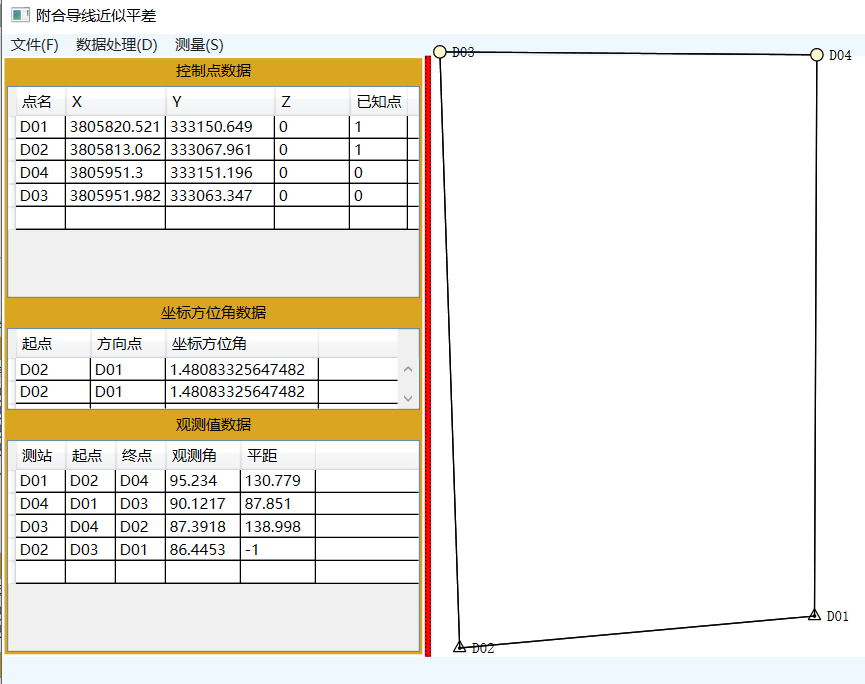
\includegraphics[scale=0.8]{chapter/connectingtraverse/ctUI01.png}
	\caption{附合导线界面功能图}
	\label{fig:ctUI01}
\end{figure}

\section{实现代码}

 \begin{lstlisting}[language=xml]
<Window x:Class="SurApp.MainWindow"
xmlns="http://schemas.microsoft.com/winfx/2006/xaml/presentation"
xmlns:x="http://schemas.microsoft.com/winfx/2006/xaml"
xmlns:local="clr-namespace:SurApp.models"
Title="附合导线近似平差" Height="350" Width="525"
WindowState="Maximized">

<DockPanel LastChildFill="True">
<Menu  x:Name="mainmenu" DockPanel.Dock="Top" Background="AliceBlue">
<MenuItem Header="文件(F)">
<MenuItem Header="新建附合导线..." Click="NewMenuItem_Click" />
<MenuItem Header="打开附合导线文件..." Click="OpenMenuItem_Click" />
<MenuItem Header="保存附合导线文件..."  Click="SaveMenuItem_Click" />
<Separator />
<MenuItem Header="导入文本数据" Click="ImportSPointMenuItem_Click"/>
<MenuItem Header="导出文本数据" Click="OutputSPointMenuItem_Click"/>
<Separator />
<MenuItem Header="导出为DXF文件" />
</MenuItem>

<MenuItem Header="数据处理(D)">
<MenuItem Header="附合导线平差" Click="AdjustMenuItem_Click" />
<MenuItem Header="平差成果" Click="AdjustResultMenuItem_Click" />
</MenuItem>

<MenuItem Header="测量(S)">
<MenuItem Header="角度弧度转换" Click="DMS2RADMenuItem_Click" />
<MenuItem Header="坐标方位角计算" Click="AzimuthMenuItem_Click" />
</MenuItem>
</Menu>
<StatusBar x:Name="statusBar" DockPanel.Dock="Bottom" Height="25"  Background="AliceBlue"/>
<Grid>
<Grid.ColumnDefinitions>
<ColumnDefinition Width="75*"/>
<ColumnDefinition Width="5"/>
<ColumnDefinition Width="170*"/>
</Grid.ColumnDefinitions>
<Border BorderThickness="2" Background="Goldenrod" Grid.Column="0">
<Grid x:Name="leftGrid" >
<Grid.RowDefinitions>
<RowDefinition Height="20"/>
<RowDefinition Height="100*"/>
<RowDefinition Height="20"/>
<RowDefinition Height="40*"/>
<RowDefinition Height="20"/>
<RowDefinition Height="100*"/>
</Grid.RowDefinitions>
<TextBlock Text="控制点数据" Grid.Row="0" TextAlignment="Center" Margin="2" />
<DataGrid x:Name="ctrPointDataGrid" Grid.Row="1" AutoGenerateColumns="False" Margin="2" ItemsSource="{Binding CtrPoints}" >
<DataGrid.Columns>
<DataGridTextColumn Header="点名" Binding="{Binding Name}" MinWidth="40"/>
<DataGridTextColumn Header="X" Binding="{Binding X , StringFormat={}{0:##0.###}}" MinWidth="60"/>
<DataGridTextColumn Header="Y" Binding="{Binding Y, StringFormat={}{0:##0.###}}" MinWidth="60" />
<DataGridTextColumn Header="Z" Binding="{Binding Z, StringFormat={}{0:##0.###}}" MinWidth="60"/>
<DataGridTextColumn Header="已知点" Binding="{Binding IsKnown}" MinWidth="30"/>
</DataGrid.Columns>
</DataGrid>

<TextBlock Text="坐标方位角数据" Grid.Row="2" TextAlignment="Center" Margin="2" />
<DataGrid x:Name="azimuthDataGrid" Grid.Row="3" AutoGenerateColumns="False" Margin="2" ItemsSource="{Binding KnownAzimuthes}" >
<DataGrid.Columns>
<DataGridTextColumn Header="起点" Binding="{Binding StartPnt.Name}" MinWidth="60"/>
<DataGridTextColumn Header="方向点" Binding="{Binding EndPnt.Name}" MinWidth="60"/>
<DataGridTextColumn Header="坐标方位角" Binding="{Binding Azimuth}" MinWidth="100" />
</DataGrid.Columns>
</DataGrid>

<TextBlock Text="观测值数据" Grid.Row="4" TextAlignment="Center" Margin="2"/>
<DataGrid x:Name="obsValueDataGrid" Grid.Row="5" AutoGenerateColumns="False"  Margin="2" ItemsSource="{Binding ObsValues}">
<DataGrid.Columns>
<DataGridTextColumn Header="测站" Binding="{Binding StnPnt.Name}" MinWidth="40"/>
<DataGridTextColumn Header="起点" Binding="{Binding StartPnt.Name}" MinWidth="40"/>
<DataGridTextColumn Header="终点" Binding="{Binding EndPnt.Name}" MinWidth="40" />
<DataGridTextColumn Header="观测角" Binding="{Binding DmsAngle}" MinWidth="60"/>
<DataGridTextColumn Header="平距" Binding="{Binding Distance}" MinWidth="60"/>
</DataGrid.Columns>
</DataGrid>

</Grid>
</Border>

<GridSplitter Background="Red" Width="5" Grid.Column="1" HorizontalAlignment="Stretch"/>

<Border BorderThickness="2" Grid.Column="2">
<local:DrawingCanvas x:Name="figureCanvas" SizeChanged="figureCanvas_SizeChanged">
<!--<Canvas.RenderTransform>
<TransformGroup>
<ScaleTransform x:Name="scaleTransform" ScaleX="1" ScaleY="-1" />
<TranslateTransform X ="0"  Y="{Binding ActualHeight, RelativeSource={RelativeSource AncestorType=Canvas}}" />
</TransformGroup>
</Canvas.RenderTransform>-->

<!--<Rectangle Height="50" Width="50" Fill="Red" Stroke="Blue" StrokeThickness="2" Canvas.Left="50" Canvas.Top="50" />

<Rectangle Height="50" Width="50" Fill="#CCCCCCFF" Stroke="Blue" StrokeThickness="2" Canvas.Left="50" Canvas.Top="50" >
<Rectangle.RenderTransform>
<TranslateTransform X="50" Y="50" />
</Rectangle.RenderTransform>
</Rectangle>-->
</local:DrawingCanvas>
</Border>
</Grid>
</DockPanel>

</Window>
 \end{lstlisting}

 \begin{lstlisting}[language=C]
using System;

namespace SurApp.models
{
[Serializable]
public class CtrPoint : ZXY.SPoint
{
private int isKnown = 0;

/// <summary>
/// 是否已知点(0:待定点, 1:已知点)
/// </summary>
public int IsKnown
	{
		get { return isKnown; }
		set
			{
				isKnown = value;
				this.RaisePropertyChange("IsKnown");
			}
	}

public CtrPoint() { }

public CtrPoint(string name, double x, double y, double z, int isKnown) : base(name, x, y, z)
{
		this.isKnown = isKnown;
	}

public override string ToString()
{
return string.Format("{0},{1},{2},{3}", Name, X, Y, Z);
}
}
}

using System;

namespace SurApp.models
{
[Serializable]
public class ObsValue : ZXY.NotificationObject
{
private CtrPoint stnPnt;
public CtrPoint StnPnt
	{
		get { return stnPnt; }
		set
			{
				stnPnt = value;
				this.RaisePropertyChange("StnPnt");
			}
	}

private CtrPoint startPnt;
public CtrPoint StartPnt
	{
		get { return startPnt; }
		set
			{
				startPnt = value;
				this.RaisePropertyChange("StartPnt");
			}
	}

private CtrPoint endPnt;
public CtrPoint EndPnt
	{
		get { return endPnt; }
		set
			{
				endPnt = value;
				this.RaisePropertyChange("EndPnt");
			}
	}

/// <summary>
///  观测角度值(单位:弧度)
/// </summary>
private double angleValue;

/// <summary>
/// 观测角度值(单位:弧度)
/// </summary>
public double AngleValue
	{
		get { return angleValue; }
		set
			{
				angleValue = value;
				this.RaisePropertyChange("DmsAngle");
				this.RaisePropertyChange("AngleValue");
			}
	}

/// <summary>
/// 观测角度值(单位:度分秒)
/// </summary>
public double DmsAngle
	{
		get { return ZXY.SMath.RAD2DMS(angleValue); }
		set
			{
				angleValue = ZXY.SMath.DMS2RAD(value);
				this.RaisePropertyChange("DmsAngle");
				this.RaisePropertyChange("AngleValue");
			}
	}


private double distance;
public double Distance
	{
		get { return distance; }
		set
			{
				distance = value;
				this.RaisePropertyChange("Distance");
			}
	}

public ObsValue() { }

public ObsValue(CtrPoint stnPnt, CtrPoint startPnt, CtrPoint endPnt,
double angleValue, double distance)
{
		this.stnPnt = stnPnt;
		this.startPnt = startPnt;
		this.endPnt = endPnt;
		this.DmsAngle = angleValue;
		this.distance = distance;
	}

private double vB; //角度改正数
public double VB
	{
		get { return vB; }
		set
			{
				vB = value;
				this.RaisePropertyChange("VB");
			}
	}

private double angleV; //改正后角度
public double AngleV
	{
		get { return angleV; }
		set
			{
				angleV = value;
				this.RaisePropertyChange("AngleV");
			}
	}

private double azimuth;
public double Azimuth
	{
		get { return azimuth; }
		set
			{
				azimuth = value;
				this.RaisePropertyChange("Azimuth");
			}
	}

private double dx;
public double DX
	{
		get { return dx; }
		set
			{
				dx = value;
				this.RaisePropertyChange("DX");
			}
	}

private double dy;
public double DY
	{
		get { return dy; }
		set
			{
				dy = value;
				this.RaisePropertyChange("DY");
			}
	}

private double vdx;
public double VDX
	{
		get { return vdx; }
		set
			{
				vdx = value;
				this.RaisePropertyChange("VDX");
			}
	}

private double vdy;
public double VDY
	{
		get { return vdy; }
		set
			{
				vdy = value;
				this.RaisePropertyChange("VDY");
			}
	}

public override string ToString()
{
return string.Format("{0},{1},{2},{3},{4}",
startPnt.Name, startPnt.Name, endPnt.Name,
DmsAngle, distance);
}
}
}

using System;
using System.Collections.Generic;
using System.Collections.ObjectModel;
using System.Windows.Media;
using ZXY;

namespace SurApp.models
{
/// <summary>
/// 用于已知边的坐标方位角信息
/// </summary>
[Serializable]
public class KnownAzimuth : NotificationObject
{
/// <summary>
/// 坐标方位角,单位:弧度
/// </summary>
public double azimuth;
public double Azimuth
	{
		get { return azimuth; }
		set
			{
				azimuth = value;
				this.RaisePropertyChange("Azimuth");
			}
	}

public CtrPoint startPnt; //坐标方位角的起点
public CtrPoint StartPnt
	{
		get { return startPnt; }
		set
			{
				startPnt = value;
				this.RaisePropertyChange("StartPnt");
			}
	}

public CtrPoint endPnt; //坐标方位角的方向点
public CtrPoint EndPnt
	{
		get { return endPnt; }
		set
			{
				endPnt = value;
				this.RaisePropertyChange("EndPnt");
			}
	}

public KnownAzimuth()
{
		startPnt = null;
		endPnt = null;
		azimuth = 0;
	}

public KnownAzimuth(CtrPoint startPnt, CtrPoint endPnt, double az)
{
		this.startPnt = startPnt;
		this.endPnt = endPnt;
		this.azimuth = az;
	}

public override string ToString()
{
if (startPnt == null || endPnt == null) return "~~~";
else
return string.Format("{0},{1},{2}", startPnt.Name, endPnt.Name, ZXY.SMath.RAD2DMS(azimuth));
}
}

[Serializable]
public class CtrNet : NotificationObject
{
private ObservableCollection<KnownAzimuth> knownAzimuthes = new ObservableCollection<KnownAzimuth>();
public ObservableCollection<KnownAzimuth> KnownAzimuthes
	{
		get { return knownAzimuthes; }
	}

private double m0 = 10; //中误差
private double fB;
private double FB; //角度闭合差的限差值
private double fx;
private double fy;
private double fs;

private double sumD;
private double K; // 1/K

//以下定义为绘图使用
private double minX;  //高斯坐标X的最小值xn
private double minY;  //高斯坐标Y的最小值yn
private double maxX; //高斯坐标X的最大值xm
private double maxY; //高斯坐标Y的最大值ym

private double maxVX; //屏幕坐标X的最大值
private double maxVY; //屏幕坐标Y的最大值

private double k;  //变换比例

private ObservableCollection<CtrPoint> ctrPoints =
new ObservableCollection<CtrPoint>();
public ObservableCollection<CtrPoint> CtrPoints
	{
		get { return ctrPoints; }
	}

private ObservableCollection<ObsValue> obsValues =
new ObservableCollection<ObsValue>();
public ObservableCollection<ObsValue> ObsValues
	{
		get { return obsValues; }
	}

/// <summary>
/// 正确的计算路线
/// </summary>
private List<ObsValue> route = new List<ObsValue>();

private bool isDirty = false;

public void ReadDataTextFile(string fileName)
{
using (System.IO.StreamReader sr = new System.IO.StreamReader(fileName))
{
string buffer;

//读入控制点数据
this.ctrPoints.Clear();
while (true)
{
		buffer = sr.ReadLine();
		if (string.IsNullOrEmpty(buffer)) break; //文件末尾或空行退出

		if (buffer[0] == '#') continue;

		string[] its = buffer.Split(new char[1] { ',' });
		if (its.Length != 4) continue; //不为四项控制点数据的继续,直到空行退出

		ctrPoints.Add(new CtrPoint(
		its[0].Trim(), // Name
		double.Parse(its[1]), //X
		double.Parse(its[2]), //Y
		double.Parse(its[3]), //H
		1)); //IsKnown
	}

//读入已知方位角信息:该节有可能不存在,也有可能有一条边,最多两条边
knownAzimuthes.Clear();
while (true)
{
		buffer = sr.ReadLine(); //由于是空行到此,所以继续往下读
		if (buffer == null) break; //文件末尾退出

		if (buffer == "" || buffer[0] == '#') continue; // 略过空行和注释行

		string[] its = buffer.Split(new char[1] { ',' });
		if (its.Length != 3) break; //数据项不为3,可能是角度观测值,退出当前

		KnownAzimuth ka = new KnownAzimuth();

		string ptName = its[0].Trim();
		ka.startPnt = GetCtrPoint(ptName);
		if (ka.startPnt == null)
		{
				ka.startPnt = new CtrPoint(ptName, 0, 0, 0, 0);//非已知点
				this.ctrPoints.Add(ka.startPnt);
			}

		ptName = its[1].Trim();
		ka.endPnt = GetCtrPoint(ptName);
		if (ka.endPnt == null)
		{
				ka.endPnt = new CtrPoint(ptName, 0, 0, 0, 0);//非已知点
				this.ctrPoints.Add(ka.endPnt);
			}

		ka.azimuth = ZXY.SMath.DMS2RAD(double.Parse(its[2]));
		knownAzimuthes.Add(ka);
	}

//读入观测值数据
this.obsValues.Clear();
while (true)
{
//此处可能由上不是3项数据的数据行退出,也有可能是文件末尾到此
//所以得先处理数据,后再读文本数据,否则,容易丢失数据
if (buffer == null) break; //文件末尾到此,继续退出
if (buffer == "" || buffer[0] == '#')//空行或正常的注释略过
{
buffer = sr.ReadLine();
continue;
}

string[] its = buffer.Split(new char[1] { ',' }); //进入正常的数据处理流程
if (its.Length == 5)
{
		string ptName = its[0].Trim();
		CtrPoint stnPnt = GetCtrPoint(ptName);
		if (stnPnt == null)
		{
				stnPnt = new CtrPoint(ptName, 0, 0, 0, 0);//非已知点
				this.ctrPoints.Add(stnPnt);
			}

		ptName = its[1].Trim();
		CtrPoint startPnt = GetCtrPoint(ptName);
		if (startPnt == null)
		{
				startPnt = new CtrPoint(ptName, 0, 0, 0, 0);//非已知点
				this.ctrPoints.Add(startPnt);
			}

		ptName = its[2].Trim();
		CtrPoint endPnt = GetCtrPoint(ptName);
		if (endPnt == null)
		{
				endPnt = new CtrPoint(ptName, 0, 0, 0, 0);//非已知点
				this.ctrPoints.Add(endPnt);
			}

		obsValues.Add(new ObsValue(
		stnPnt, startPnt, endPnt,
		double.Parse(its[3]), //AngleValue
		double.Parse(its[4]))); //Distance
	}

buffer = sr.ReadLine();
}
}
}

public void WriteDataTextFile(string fileName)
{
		using (System.IO.StreamWriter sw = new System.IO.StreamWriter(fileName))
		{
				sw.WriteLine("# Name, X, Y, Z");
				foreach (var pt in this.ctrPoints)
				{
						if(pt.IsKnown == 1) sw.WriteLine( pt );
					}

				sw.WriteLine();
				sw.WriteLine("# StartPnt, EndPnt, Azimuth");
				foreach (var az in this.knownAzimuthes)
				{
						sw.WriteLine( az );
					}

				sw.WriteLine();
				sw.WriteLine("# Station, StartPnt, EndPnt, Angle, Distance");
				foreach (var obs in this.ObsValues)
				{
						sw.WriteLine( obs );
					}
			}
	}


private ObsValue SearchStartObsValue()
{
		/**
		* 搜索起始边,首先:搜索直接给定的坐标方位角
		* 其次:上述搜索不成立的情况,搜索:测站点与后视点均为已知点的观测值
		* 再次:反向搜索:测站点与后视点均为已知点的观测值
		* */
		ObsValue obs = null;

		if (this.knownAzimuthes.Count > 0)
		{
				foreach (var azi in this.knownAzimuthes)
				{
						if (azi.endPnt.IsKnown == 1)
						{
								foreach (var it in obsValues)
								{
										if (it.StartPnt == azi.startPnt && it.StnPnt == azi.endPnt)
										{
												obs = it;
												return obs;
											}
									}
							}
					}
			}
		else if (this.knownAzimuthes.Count == 0)
		{
				foreach (var it in obsValues)
				{
						double az = 0;

						if (it.StartPnt.IsKnown == 1 && it.StnPnt.IsKnown == 1)
						{
								az = ZXY.SMath.Azimuth(it.StartPnt.X, it.StartPnt.Y, it.StnPnt.X, it.StnPnt.Y);
								this.knownAzimuthes.Add(new KnownAzimuth(it.StartPnt, it.StnPnt, az));
								obs = it;
							}

						if (it.StnPnt.IsKnown == 1 && it.EndPnt.IsKnown == 1)
						{
								az = ZXY.SMath.Azimuth(it.StnPnt.X, it.StnPnt.Y, it.EndPnt.X, it.EndPnt.Y);
								this.knownAzimuthes.Add(new KnownAzimuth(it.StnPnt, it.EndPnt, az));
							}
					}
			}
		return obs;
	}


/// <summary>
/// 递归搜索观测值obs0的下一条边
/// </summary>
/// <param name="obs0">当前观测值</param>
/// <returns>1:附合导线, -1:不构成附合导线</returns>
private int SearchObsValue(ObsValue obs0)
{
//传进来的第一条边应为起始边
ObsValue obsi = null;

foreach (var it in obsValues)
{
if (it == obs0) continue;

if (obs0.StnPnt == it.StartPnt && obs0.EndPnt == it.StnPnt)  //满足条件的下一条边
{
obsi = it;
break;
}
}

if (obsi == null) return -1;//没找到这样的边

this.route.Add(obsi);
if (obsi.StnPnt.IsKnown == 1 && obsi.EndPnt.IsKnown == 1) //附合到另一条已知边了,退出
{
return 1;
}
else
SearchObsValue(obsi); //递归继续寻找下一条这样的边

return 0;
}


/// <summary>
/// 搜索正确的计算路线
/// </summary>
/// <returns>是否成功</returns>
public bool SearchCalRoute()
{
		ObsValue obs0 = SearchStartObsValue();
		if (obs0 == null) return false;

		route.Clear(); //清空搜索线路

		route.Add(obs0);
		SearchObsValue(obs0);
		return true;
	}

/// <summary>
/// 简易平差
/// </summary>
/// <returns>0:成功</returns>
public int Adjust()
{
		/*
		1. 求起始边: 后视->测站 的方位角
		求末边:测站->前视 的方位角
		2. 计算角度闭合差fB,FB
		3. 改正角度值
		4. 推算各边坐标方位角
		5. 计算各边的坐标增量
		6.计算fx, fy, fs, 1/K
		7.计算改正后的坐标增量
		8.计算各点的坐标值
		*/
		if (this.obsValues.Count == 0) return -1; //观测值为空

		if (SearchCalRoute() == false) return -2; //搜索不到正确的附合路线

		double az0 = this.knownAzimuthes[0].azimuth;
		CtrPoint startPnt0 = this.knownAzimuthes[0].startPnt;
		CtrPoint stnPnt0 = this.knownAzimuthes[0].endPnt;

		double azn = this.knownAzimuthes[1].azimuth;
		CtrPoint stnPntn = this.knownAzimuthes[1].startPnt;
		CtrPoint endPntn = this.knownAzimuthes[1].endPnt;

		double azi = az0;
		double n = route.Count;
		foreach (var obs in route) //foreach (var obs in this.ObsValues)
		{
				obs.Azimuth = azi + obs.AngleValue + Math.PI;
				if (obs.Azimuth >= 2 * Math.PI) obs.Azimuth -= 2 * Math.PI;
				if (obs.Azimuth < 0) obs.Azimuth += 2 * Math.PI;

				azi = obs.Azimuth;
			}

		fB = azi - azn; //单位:弧度
		FB = m0 * 2 * Math.Sqrt(n); //单位:秒

		//改正角度,推算各边改正后的方位角
		azi = az0;
		double vi = -fB / n;
		foreach (var obs in route) //foreach (var obs in this.ObsValues)
		{
				obs.VB = vi;
				obs.AngleV = obs.AngleValue + obs.VB;
				obs.Azimuth = azi + obs.AngleV + Math.PI;
				if (obs.Azimuth >= 2 * Math.PI) obs.Azimuth -= 2 * Math.PI;
				if (obs.Azimuth < 0) obs.Azimuth += 2 * Math.PI;
				azi = obs.Azimuth;
			}

		//计算各边的坐标增量
		double sumDX = 0, sumDY = 0;
		sumD = 0;
		foreach (var obs in route) //foreach (var obs in this.ObsValues)
		{
				if (obs.Distance <= 0) continue;

				obs.DX = obs.Distance * Math.Cos(obs.Azimuth);
				obs.DY = obs.Distance * Math.Sin(obs.Azimuth);
				sumDX += obs.DX;
				sumDY += obs.DY;
				sumD += obs.Distance;
			}
		fx = stnPnt0.X + sumDX - stnPntn.X;
		fy = stnPnt0.Y + sumDY - stnPntn.Y;
		fs = Math.Sqrt(fx * fx + fy * fy);
		K = sumD / fs;

		//改正坐标增量,计算各点坐标
		foreach (var obs in route) //foreach (var obs in this.ObsValues)
		{
				if (obs.Distance <= 0) continue;

				obs.VDX = -fx / sumD * obs.Distance;
				obs.VDY = -fy / sumD * obs.Distance;

				obs.EndPnt.X = obs.StnPnt.X + obs.DX + obs.VDX;
				obs.EndPnt.Y = obs.StnPnt.Y + obs.DY + obs.VDY;
			}

		return 0;
	}

private CtrPoint GetCtrPoint(string pointName)
{
		foreach (var pt in this.ctrPoints)
		{
				if (pt.Name == pointName)
				return pt;
			}

		return null;
	}

public void OnDraw(DrawingCanvas canvas)
{
		if (this.ctrPoints.Count < 1) return;

		GetGaussXySize();

		maxVX = canvas.ActualWidth-20;
		maxVY = canvas.ActualHeight;

		double kx = maxVX / (maxY - minY);
		double ky = maxVY / (maxX - minX);
		k = kx <= ky ? kx : ky;

		canvas.ClearAll(); //先清除屏幕

		//画观测值
		double x0, y0, x1, y1, x2, y2; //画直线的两个端点
		foreach (var it in this.obsValues)
		{
				if (it.StnPnt.X <= 0 && it.StnPnt.Y <= 0) continue; //略过坐标为0的点
				GaussXyToViewXy(it.StnPnt.X, it.StnPnt.Y, out x0, out y0);

				if (it.StartPnt.X > 0 && it.StartPnt.Y > 0)
				{
						GaussXyToViewXy(it.StartPnt.X, it.StartPnt.Y, out x1, out y1);
						canvas.DrawLine(x1, y1, x0, y0, Brushes.Black, 1);
					}

				if (it.EndPnt.X > 0 && it.EndPnt.Y > 0)
				{
						GaussXyToViewXy(it.EndPnt.X, it.EndPnt.Y, out x2, out y2);
						canvas.DrawLine(x0, y0, x2, y2, Brushes.Black, 1);
					}
			}

		//再画控制点
		foreach (var pt in this.ctrPoints)
		{
				if (pt.X <= 0 && pt.Y <= 0) continue; //排除坐标为0的点

				GaussXyToViewXy(pt.X, pt.Y, out x0, out y0);
				if(pt.IsKnown == 1)
				canvas.DrawKnCtrPnt(x0, y0, Brushes.Black, 1);
				else
				canvas.DrawCtrPnt(x0, y0, Brushes.Black, 1);
				canvas.DrawText(pt.Name, x0 + 10, y0 - 7);
			}
	}

private void GaussXyToViewXy(double xt, double yt, out double xp, out double yp)
{
		//xp = x0 + kx(yt - yn);
		//yp = y1 - (y0 + ky * (xt - xn));
		// x0 = y0 =0 且 kx = ky =k, 故以上公式简化为:

		xp = 5 + k * (yt - minY); //x0 = 5;
		yp = maxVY - (5 + k * (xt - minX)); //y0=5;
	}

private void GetGaussXySize()
{
minX = this.ctrPoints[0].X; minY = this.ctrPoints[0].Y;
maxX = this.ctrPoints[0].X; maxY = this.ctrPoints[0].Y;

for (int i = 1; i < this.ctrPoints.Count; i++) //如果只有一个点,由循环条件知,不会执行循环体
{
if (this.ctrPoints[i].X <= 0 && this.ctrPoints[i].Y <= 0) continue;

if (this.ctrPoints[i].X < minX) minX = this.ctrPoints[i].X;
if (this.ctrPoints[i].Y < minY) minY = this.ctrPoints[i].Y;

if (this.ctrPoints[i].X > maxX) maxX = this.ctrPoints[i].X;
if (this.ctrPoints[i].Y > maxY) maxY = this.ctrPoints[i].Y;
}

//针对一个点或点范围较小的情况,进行范围扩展
if (minX + 10 > maxX) { maxX = minX + 10; minX = maxX - 20; }
if (minY + 10 > maxY) { maxY = minY + 10; minY = maxY - 20; }
}
}
}

using System.Globalization;
using System.Windows;
using System.Windows.Media;

namespace SurApp.models
	{
		public class DrawingCanvas : System.Windows.Controls.Canvas
			{
				private VisualCollection visuals;

				public DrawingCanvas()
				{
						visuals = new VisualCollection(this);
					}

				//获取Visual的个数
				protected override int VisualChildrenCount
					{
						get { return visuals.Count; }
					}

				//获取Visual
				protected override Visual GetVisualChild(int index)
				{
						return visuals[index];
					}

				//添加Visual
				public void AddVisual(Visual visualObject)
				{
						visuals.Add( visualObject );
					}

				//删除Visual
				public void RemoveVisual(Visual visualObject)
				{
						base.RemoveLogicalChild(visualObject);
					}

				//命中测试
				public DrawingVisual GetVisual(System.Windows.Point point)
				{
						HitTestResult hitResult = VisualTreeHelper.HitTest(this, point);
						return hitResult.VisualHit as DrawingVisual;
					}

				public void ClearAll()
				{
						this.visuals.Clear();
					}


				//使用DrawVisual画Polyline
				public void DrawLine(double x0, double y0, double x1, double y1,  Brush color, double thinkness)
				{
						DrawingVisual visualLine = new DrawingVisual();
						DrawingContext dc = visualLine.RenderOpen();
						Pen pen = new Pen(color, thinkness);
						pen.Freeze();  //冻结画笔,这样能加快绘图速度
						dc.DrawLine(pen, new Point(x0, y0),  new Point(x1, y1) );

						dc.Close();
						visuals.Add(visualLine);
					}

				public void DrawText(string text, double x, double y)
				{
						DrawingVisual visualText = new DrawingVisual();
						DrawingContext dc = visualText.RenderOpen();
						Typeface tp = new Typeface(new FontFamily("宋体"), FontStyles.Normal, FontWeights.Normal, FontStretches.Normal);
						FormattedText ft = new FormattedText(text, CultureInfo.CurrentCulture,
						FlowDirection.LeftToRight, tp, 12, Brushes.Black);
						dc.DrawText(ft, new Point(x, y) );
						dc.Close();
						visuals.Add( visualText );
					}

				//使用DrawVisual画Circle,用作控制点
				public void DrawCtrPnt(double x, double y,  Brush color, double thinkness)
				{
						DrawingVisual visualCircle = new DrawingVisual();
						DrawingContext dc = visualCircle.RenderOpen();
						Pen pen = new Pen(color, thinkness);
						pen.Freeze();  //冻结画笔,这样能加快绘图速度
						dc.DrawEllipse(Brushes.LemonChiffon,  pen,  new Point(x, y),  5, 5);
						dc.Close();
						visuals.Add(visualCircle);
					}

				//使用DrawVisual画Circle,用作控制点
				public void DrawKnCtrPnt(double x, double y, Brush color, double thinkness)
				{
						DrawingVisual visualCircle = new DrawingVisual();
						DrawingContext dc = visualCircle.RenderOpen();
						Pen pen = new Pen(color, thinkness);
						pen.Freeze();  //冻结画笔,这样能加快绘图速度
						dc.DrawEllipse(Brushes.Black, pen, new Point(x, y), 1, 1);
						dc.DrawLine(pen, new Point(x-5, y+2.9), new Point(x+5, y+2.9));
						dc.DrawLine(pen, new Point(x + 5, y + 2.9), new Point(x, y - 5.8));
						dc.DrawLine(pen, new Point(x, y - 5.8), new Point(x - 5, y + 2.9));
						dc.Close();
						visuals.Add(visualCircle);
					}
			}
	}

 \end{lstlisting}
 %%附合导线近似平差程序设计
%!TEX root = ../../clcxsj.tex

\chapter{线路要素计算程序设计}

\section{圆曲线程序设计}

\subsection{圆曲线的数学模型与算法分析}

\begin{figure}[htbp]
    \centering
    \subfloat[左偏]
    {
        \label{fig:CircleRoute-Left}
        \includegraphics[scale=0.7]{chapter/route/LeftCircleRoute.pdf}
    }
    \hspace{1pt} %
    \subfloat[右偏]
    {
        \label{fig:CircleRoute-Right}
        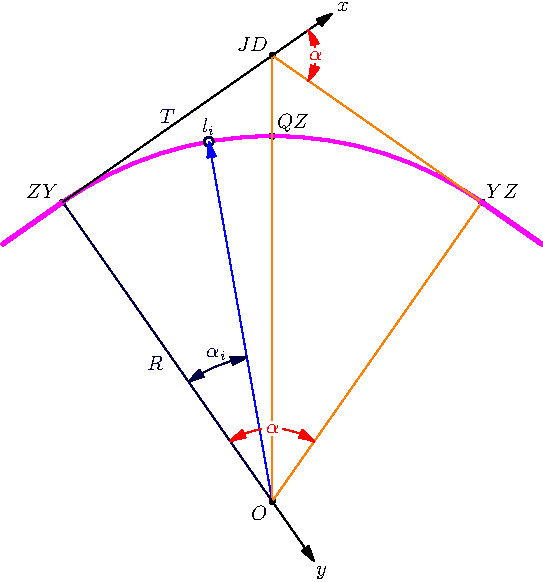
\includegraphics[scale=0.7]{chapter/route/RightCircleRoute.pdf}
    }
    \caption{圆曲线要素图}
    \label{fig:CircleRoute}
\end{figure}


% \begin{figure}[htbp]
%     \centering
%     \includegraphics[scale=0.8]{route/LeftCircleRoute.pdf}
%     \caption{左偏-圆曲线要素图}
%     \label{fig:LeftCircleRoute}
% \end{figure}

% \begin{figure}[htbp]
%     \centering
%     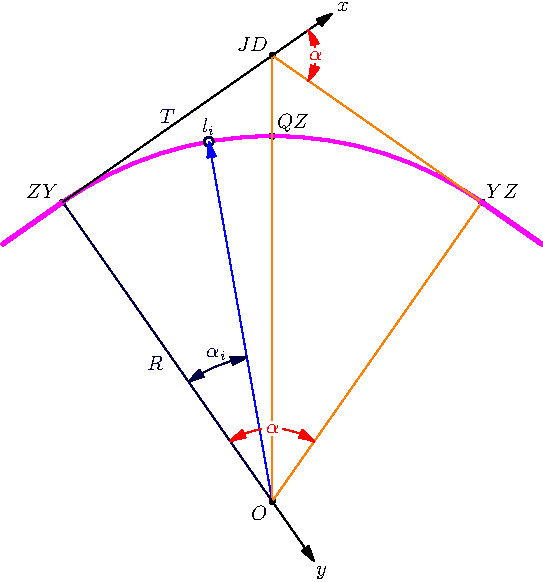
\includegraphics[scale=0.8]{chapter/route/RightCircleRoute.pdf}
%     \caption{右偏-圆曲线要素图}
%     \label{fig:RightCircleRoute}
% \end{figure}

圆曲线的各个要素计算算法如下:

 切线长:$T = R \cdot \tan (\alpha / 2)$

 曲线长:$L = R \cdot \alpha$

 外矢距:$E=R \cdot (\sec (\alpha /2) - 1)$

 切曲差:$q = 2T - L$

 \subsection{圆曲线上点的坐标计算算法分析}

 全站仪的坐标放样模式与 GPS RTK 可以十分方便的进行圆曲线上点的坐标放样。

 尽管圆曲线的计算方法有很多,也比较简单,但为了与后边的缓和曲线计算方法相一致,
 我们在此采用圆心角加半径再加坐标系转换法进行圆曲线上点的坐标计算。

 如图\ref{fig:CircleRoute}所示,以ZY点为原点,以ZY至JD切线方向为x轴,
 以ZY至O点方向为y轴建立ZY切线测量坐标系。从(a)与(b)两图可以看出
无论圆曲线是左偏还是右偏的,其坐标系是一致的。
 在ZY切线坐标系中用极坐标法按如下公式可以计算出圆曲线上任意一点$l_i$的坐标。

圆曲线偏左:

\begin{equation}
\left .
\begin{aligned}
x_{i} &= R \sin \alpha_i   \\
y_{i} &= -R(1- \cos \alpha_i)
\end{aligned}
\right \}
\label{eq:ZYLeftXY}
\end{equation}

圆曲线偏右:

\begin{equation}
\left .
\begin{aligned}
x_{i} &= R \sin \alpha_i   \\
y_{i} &= R(1- \cos \alpha_i)
\end{aligned}
\right \}
\label{eq:ZYRightXY}
\end{equation}

式中:$\alpha_i = l_i / R,  \alpha_i \le \alpha $, $l_i$可用圆曲线上任意一点的里程桩号
减去ZY点的里程桩号。

如果我们以偏右为正、偏左为负,则可以将以上两公式统一,将偏左的Y坐标
乘以 -1 即可。

已知JD的坐标与里程桩号,根据圆曲线的结合几何要素$R, \alpha$即可计算出圆曲线上特征点的
里程桩号:

$KNo_{ZY} = KNo_{JD} - T$

$KNo_{QZ} = KNo_{ZY} + T/2$

$KNo_{YZ} = KNo_{QZ} + T/2$

在ZY切线坐标系中计算出圆曲线上各点的坐标之后,还需将其转换为测量坐标系
(或更正式的称为大地坐标系或独立施工坐标系)。在前一章我们已经做过坐标系的
转换了,在这个线路转换中,我们将ZY-JD边定义为x轴,因此两坐标系的夹角
即为ZY-JD边的坐标方位角,其转换关系如图\ref{fig:xytoxyroute}所示:

\begin{figure}[htbp]
    \centering
    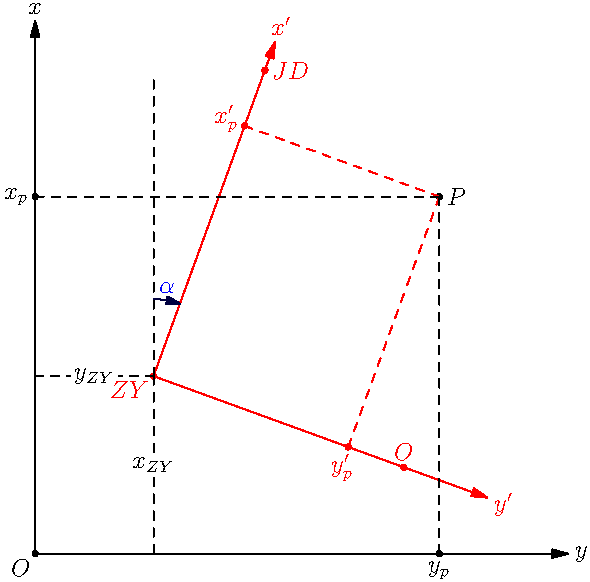
\includegraphics[scale=0.8]{chapter/route/xytoxyroute.pdf}
    \caption{ZY坐标系转测量坐标系}
    \label{fig:xytoxyroute}
\end{figure}

转换公式如下:

\begin{equation}
\left .
\begin{aligned}
x_{P} &= x_{ZY} + x'_P \cos \alpha - y'_P \sin \alpha  \\
y_{P} &= y_{ZY} + x'_P \sin \alpha + y'_P \cos \alpha
\end{aligned}
\right \}
\label{eq:routexytoxy}
\end{equation}


\subsection{圆曲线坐标计算中的类设计}

由以上分析可知,线路计算中至少应该有点类 GPoint 和 线路类 CircleRoute 。

\begin{enumerate}
\item 程序中的点类GPoint

线路上的GPoint 类应包含序号、里程桩号、X坐标、Y坐标、备注信息等内容。
我们设计如下:

\begin{lstlisting}[language=C]
using System;
namespace Route.models
{
    /// <summary>
    /// 点类
    /// </summary>
    public class GPoint : NotificationObject
    {
        private int _no;
        /// <summary>
        /// 序号
        /// </summary>
        public int No
        {
            get { return _no; }
            set
            {
                _no = value;
                RaisePropertyChange("No");
            }
        }

        private double _kno;
        /// <summary>
        /// 里程桩号
        /// </summary>
        public double KNo
        {
            get { return _kno; }
            set
            {
                _kno = value;
                RaisePropertyChange("KNo");
            }
        }

        private double _x;
        /// <summary>
        /// X坐标
        /// </summary>
        public double X
        {
            get { return _x; }
            set
            {
                _x = value;
                RaisePropertyChange("X");
            }
        }

        private double _y;
        /// <summary>
        /// Y坐标
        /// </summary>
        public double Y
        {
            get { return _y; }
            set
            {
                _y = value;
                RaisePropertyChange("Y");
            }
        }

        private string _note;
        /// <summary>
        /// 备注
        /// </summary>
        public string Note
        {
            get { return _note; }
            set
            {
                _note = value;
                RaisePropertyChange("Note");
            }
        }

        public GPoint()
        {
            _no = 0;
            _kno = _x = _y = 0;
            _note = "";
        }
    }
}
\end{lstlisting}

在上面GPoint类中,由于点的里程桩号是double类型,而我们常用的里程桩号是
``K5+200.00''这样的形式,因此我们在类GPoint中设计函数OutKNoInfo()
将其转换输出,其代码如下所示:

\begin{lstlisting}[language=C]
public class GPoint : NotificationObject
{
    //......类中其它代码......

    /// <summary>
    /// 将double类型的kno分解为K5+200.00形式的里程桩号
    /// </summary>
    /// <returns>里程桩号</returns>
    public string OutKNoInfo()
    {
        int k = (int)(_kno / 1000);
        double klength = _kno - k * 1000;
        return string.Format("K{0}+{1:0.000}", k, klength);
    }
}
\end{lstlisting}

以上代码的逻辑非常简单,double类型的里程除以1000,取出公里数,
然后将不足整公里数的部分再取出,然后组合成形如``K5+200.00''这样的
字符串输出。

由于以上代码只涉及类中的 \_kno 字段,因此也可以写成如下的只读属性字段,
调用会更加方便。

\begin{lstlisting}[language=C]
public class GPoint : NotificationObject
{
    //......类中其它代码......

    /// <summary>
    /// 将double类型的kno分解为K5+200.00形式的里程桩号
    /// </summary>
    public string KNoInfo
    {
        get{
            int k = (int)(_kno / 1000);
            double klength = _kno - k * 1000;
            return string.Format("K{0}+{1:0.000}", k, klength);
        }
    }
}
\end{lstlisting}

\item 程序中的圆曲线类CircleRoute

圆曲线类中应包含偏转角$\alpha$、曲率半径R、切线长$T$等基本属性,
还应包括JD点、ZY点、QZ点、YZ点等属性,设计代码如下:

\begin{lstlisting}[language=C]
public class CircleRoute : NotificationObject
{
    private double _alpha;
    /// <summary>
    /// 偏转角,单位:度分秒
    /// </summary>
    public double alpha
    {
        get { return _alpha; }
        set
        {
            _alpha = value;
            RaisePropertyChange("alpha");
        }
    }

    protected double _R;
    /// <summary>
    /// 圆曲线半径
    /// </summary>
    public double R
    {
        get { return _R; }
        set
        {
            _R = value;
            RaisePropertyChange("R");
        }
    }

    double _T;
    /// <summary>
    /// 切线长
    /// </summary>
    public double T
    {
        get { return _T; }
        set
        {
            _T = value;
            RaisePropertyChange("T");
        }
    }

    double _L;
    /// <summary>
    /// 曲线长
    /// </summary>
    public double L
    {
        get { return _L; }
        set
        {
            _L = value;
            RaisePropertyChange("L");
        }
    }

    double _E;
    /// <summary>
    /// 外矢距
    /// </summary>
    public double E
    {
        get { return _E; }
        set
        {
            _E = value;
            RaisePropertyChange("E");
        }
    }

    double _q;
    /// <summary>
    /// 切曲差
    /// </summary>
    public double q
    {
        get { return _q; }
        set
        {
            _q = value;
            RaisePropertyChange("q");
        }
    }

    GPoint _JD = new GPoint();
    /// <summary>
    /// 交点
    /// </summary>
    public GPoint JD
    {
        get { return _JD; }
        set
        {
            _JD = value;
            RaisePropertyChange("JD");
        }
    }

    GPoint _QZ = new GPoint();
    /// <summary>
    /// 曲中点
    /// </summary>
    public GPoint QZ
    {
        get { return _QZ; }
        set
        {
            _QZ = value;
            RaisePropertyChange("QZ");
        }
    }

    GPoint _ZY = new GPoint();
    /// <summary>
    /// 直圆点
    /// </summary>
    public GPoint ZY
	{
		get { return _ZY; }
		set
		{
			_ZY = value;
			RaisePropertyChange("ZY");
		}
	}

    GPoint _YZ = new GPoint();
    /// <summary>
    /// 圆直点
    /// </summary>
    public GPoint YZ
	{
		get { return _YZ; }
		set
		{
			_YZ = value;
			RaisePropertyChange("YZ");
		}
    }

    private int _isLeftRight = 1;
    /// <summary>
    /// 左偏:-1 或 右偏:1
    /// </summary>
    public int IsLeftRight
	{
		get { return _isLeftRight; }
		set
			{
				_isLeftRight = value;
				RaisePropertyChange("IsLeftRight");
			}
    }

    /// <summary>
    /// 线路点集
    /// </summary>
    protected ObservableCollection<GPoint> _pointList =
        new ObservableCollection<GPoint>();

    /// <summary>
    /// 线路点集
    /// </summary>
    public ObservableCollection<GPoint> PointList
    {
        get { return _pointList; }
    }
}
\end{lstlisting}

在圆曲线计算时,由于左偏与右偏的计算是不完全相同的,在此设计一
属性IsLeftRight用来标记。

为了存储计算后的点坐标,我们设计了一点集属性PointList。
\end{enumerate}

\subsection{ 任意桩号点的坐标计算 }

给定任意一桩号,计算圆曲线上点的坐标,函数设计如下:
\begin{lstlisting}[language=C]
/// <summary>
/// 计算任意里程桩号的点坐标
/// </summary>
/// <param name="kno">里程桩号</param>
public void CalSinglePoint(double kno)
{
    double radAlpha = ZXY.SMath.DMS2RAD(alpha);
    T = R * Math.Tan(radAlpha * 0.5);
    L = R * radAlpha;
    E = R * (1 / Math.Cos(radAlpha * 0.5) - 1);

    ZY.KNo = JD.KNo - T;
    QZ.KNo = ZY.KNo + L/2;
    YZ.KNo = QZ.KNo + L/2;

    double li = kno - ZY.KNo;
    if( li<0 || li>L) return; //不是圆曲线上有效范围
    double alphai = li / R;

    GPoint pt = new GPoint();
    pt.KNo = kno;

    pt.X = R * Math.Sin(alphai);
    pt.Y = IsLeftRight * R * (1 - Math.Cos(alphai));

    double A = ZXY.SMath.Azimuth(ZY.X, ZY.Y, JD.X, JD.Y);
    pt.TransformXY(ZY.X, ZY.Y, A); //转换到大地坐标

    PointList.Add(pt); //将计算结果存入PointList
}
\end{lstlisting}

在该算法中,第7行将度分秒形式的偏转角转换为弧度,再根据
前边的算法计算圆曲线的几何要素T、L、E等。

一般情况下JD的里程桩号与坐标是已知的,直圆点ZY的坐标也会已知,但里程桩号
未知,所以需要首先计算出ZY点的里程桩号。同样的道理也可以计算出曲中点QZ与圆
直点YZ点的里程桩号。

第16行根据给定的里程桩号与ZY点的里程桩号计算圆曲线的弧长$l_i$,
第17行做有效性判断:$0 \le l_i \le L$),
第18行根据弧长计算该点所在位置的圆心角$\alpha_i$。

第23、24行根据公式 \ref{eq:ZYRightXY} 计算圆曲线上各点在ZY坐标系
中的各点坐标。如果圆曲线偏左,根据公式 \ref{eq:ZYLeftXY} 将其Y坐标乘以
 -1 即IsLeftRight的属性值即可。

第26行计算出ZY点至JD点的坐标方位角,第27行根据公式\ref{eq:routexytoxy}将其
转换到大地坐标系。

第29行将其加入到PointList列表中,用于界面显示。

\subsection{圆曲线算例与测试代码}
圆曲线的曲率半径为$R=120m$,偏转角为$\alpha=40^{\degree}20'$, 交点JD
的里程桩号为``K3+135.12'',坐标为$(6848.320, 5634.240)$;
直圆点ZY的坐标为$(6821.354,5599.381)$。计算出的圆曲线上各点坐标
如表\ref{tab:YRoute}所示。

\begin{table}[htbp]
\centering
\caption{圆曲线计算示例数据表}
\label{tab:YRoute}
\begin{tabular}{clccl}
\hline
序号  &  里程     &     X    &   Y	  & 备注 \\
\hline
1    & K3+091.05 &  6821.35 & 5999.38 &  ZY \\
2    & K3+100	 & 	6826.56 & 5606.66 &     \\
3    & K3+120	 &  6836.15 & 5624.18 &     \\
4    & K3+133.29 &  6840.85 & 5636.60 &  QZ \\
5    & K3+140	 & 	6842.69 & 5643.06 &     \\
6    & K3+160	 &  6846.02 & 5662.76 &     \\
7    & K3+175.52 &  6846.31 & 5678.27 &  YZ \\
\hline
\end{tabular}
\end{table}

测试代码为:
\begin{lstlisting}[language=C]
models.CircleRoute route = new models.CircleRoute();
route.R = 120;
route.alpha = 40.20;
route.IsLeftRight = 1;

route.JD.X = 6848.320;
route.JD.Y = 5634.240;
route.JD.KNo = 3135.12;

route.ZY.X = 6821.354;
route.ZY.Y = 5599.381;

route.CalSinglePoint(3175.52);
\end{lstlisting}

\subsection{线路上的点按间距批量计算}

除了能进行任意里程桩号的计算外,线路计算程序还应该支持按指定间隔进行
批量计算的功能。在批量计算中,还应该将线路特征点的坐标计算并显示出来,
并按照里程桩号的顺序进行排列。


\subsection{界面的实现}

程序的界面编写我们仍采用WPF技术,布局如图...所示:


\section{有缓和曲线的圆曲线}

有缓和曲线的圆曲线的数学模型与算法相对于圆曲线来说就复杂多了。
下面我们将从算法到程序实现逐一分析。

\subsection{缓和曲线的数学模型}

 \begin{figure}[htbp]
    \centering
    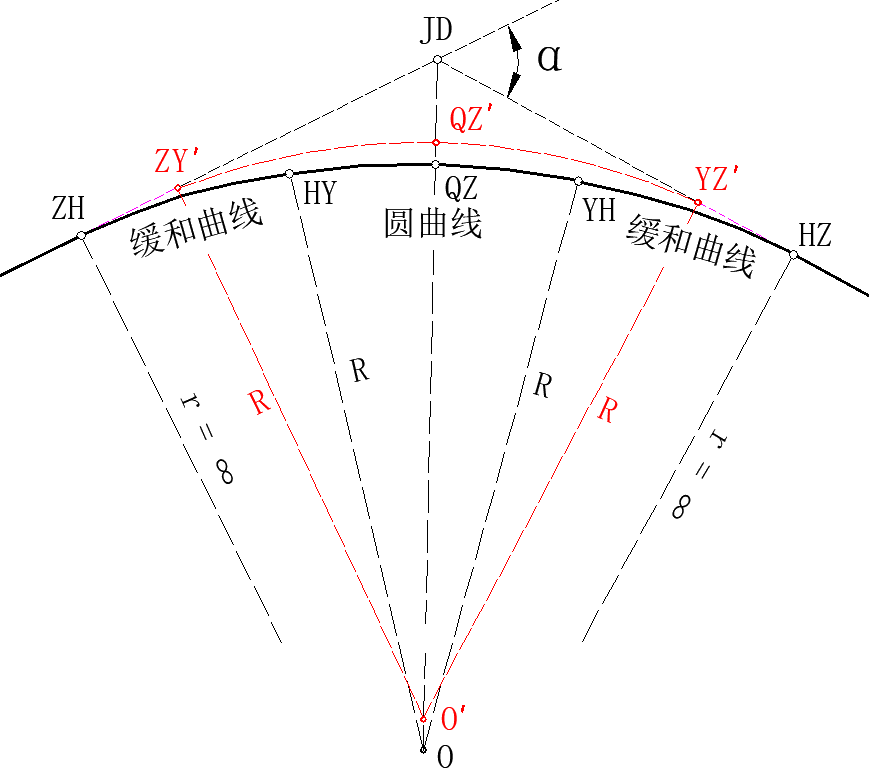
\includegraphics[scale=0.6]{chapter/route/HY01.png}
    \caption{缓和曲线的定义}
    \label{fig:HR01}
\end{figure}


\begin{figure}[htbp]
    \centering
    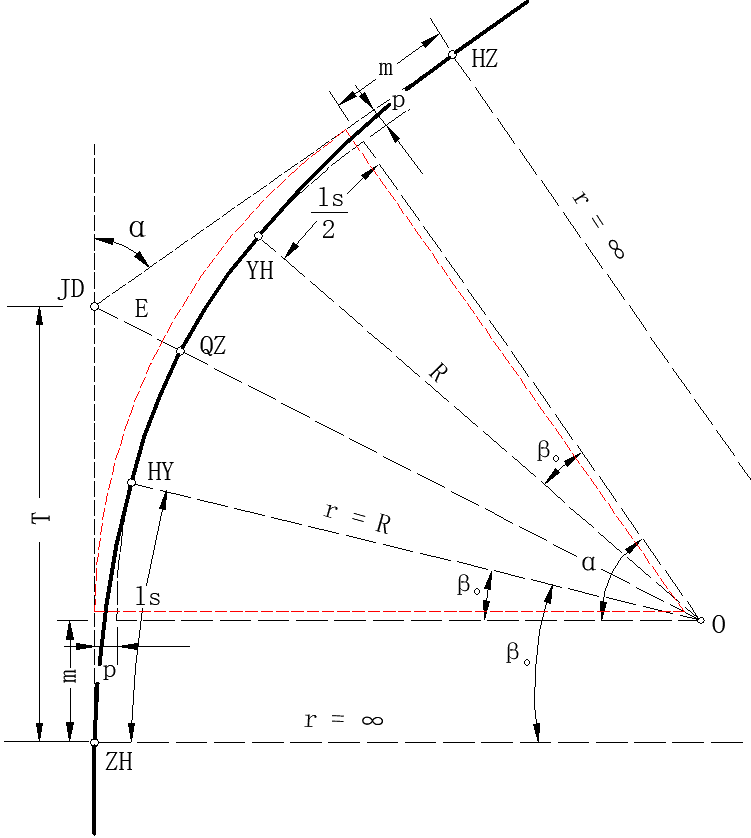
\includegraphics[scale=0.6]{chapter/route/HY02.png}
    \caption{缓和曲线的内移距和切线增长}
    \label{fig:HY02}
\end{figure}


\begin{figure}[htbp]
    \centering
    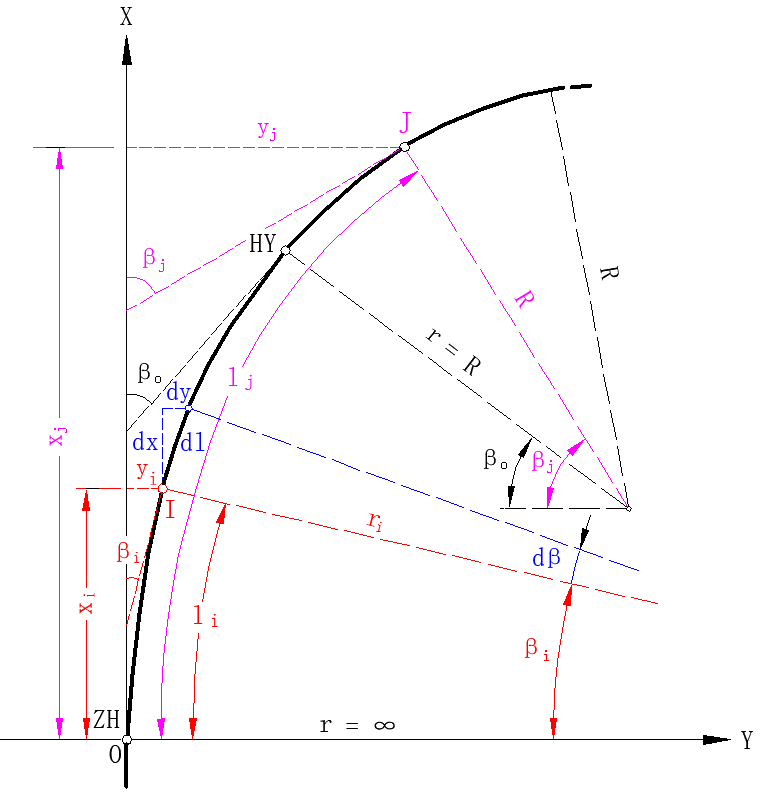
\includegraphics[scale=0.6]{chapter/route/HY03.png}
    \caption{缓和曲线的坐标计算}
    \label{fig:HR03}
\end{figure}

 缓和曲线参数计算公式为:

 $$\beta_0 = \frac{l_0}{2R} $$
切垂距:
$$m=\frac{l_0}{2} - \frac{l^3_0}{240R^2}$$
内移距:
$$p=\frac{l^2_0}{24R}$$


 切线长:$$T = m+ (R+p) \cdot \tan \frac{\alpha}{2}$$

 曲线全长:$$L = R \cdot (\alpha-2\beta_0)  + 2l_0$$

 圆曲线长:$$L_C = R \cdot (\alpha-2\beta_0)$$

 外矢距:$$E=(R+p) \cdot (\sec \frac{\alpha}{2} - 1)$$

\begin{enumerate}

\item  缓和曲线在ZH切线直角坐标系中的坐标计算(ZH段)

以ZH为坐标系原点,ZH至JD方向为x轴,过ZH点垂直于ZH-JD方向为y轴
建立坐标,如图\ref{fig:HY02}所示。则ZH部分缓和曲线上各点的坐标为:

\begin{equation}
\left .
\begin{aligned}
x_i &= l_i - \frac{l^5_i}{40R^2 l^2_0} + \frac{l^9_i}{3456R^4 l^4_0}
           - \frac{l^{13}_i}{599040R^6l^6_0} + ...  \\
y_i &=  \frac{l^3_i}{6Rl_0} - \frac{l^7_i}{336R^3 l^3_0}
    + \frac{l^{11}_i}{42240R^5l^5_0} -\frac{l^{15}_i}{9676800R^7l^7_0}+ ...
\end{aligned}
\right \}
\label{eq:routeZHXY}
\end{equation}

以上公式在计算中取前两项或前三项即可。

\item  缓圆点(HY)坐标计算公式为:

将$l_i = l_0$代入公式\ref{eq:routeZHXY}中计算可得到下式:
\begin{equation}
\left . \begin{aligned}
x_{HY} &= l_0 - \frac{l^3_0}{40R^2} + \frac{l^5_0}{3456R^4}
          - \frac{l^{7}_0}{599040R^6} + ...  \\
y_{HY} &=  \frac{l^2_0}{6R} - \frac{l^4_0}{336R^3}
          + \frac{l^{6}_i}{42240R^5} -\frac{l^{8}_0}{9676800R^7}+ ...
\end{aligned} \right \}
\label{eq:routeHY}
\end{equation}

\item  圆曲线上点的坐标计算公式为:

\begin{equation}
\left . \begin{aligned}
x_{j} &= R \sin \beta_j + m \\
y_{j} &= R(1- \cos \beta_j) +p
\end{aligned} \right \}
\label{eq:routeYQXY}
\end{equation}

式中:$\beta_i = \beta_0 + (l_i - l_0)/R$

\item  缓和曲线在HZ切线直角坐标系中的坐标计算(HZ段)

\begin{figure}[htbp]
    \centering
    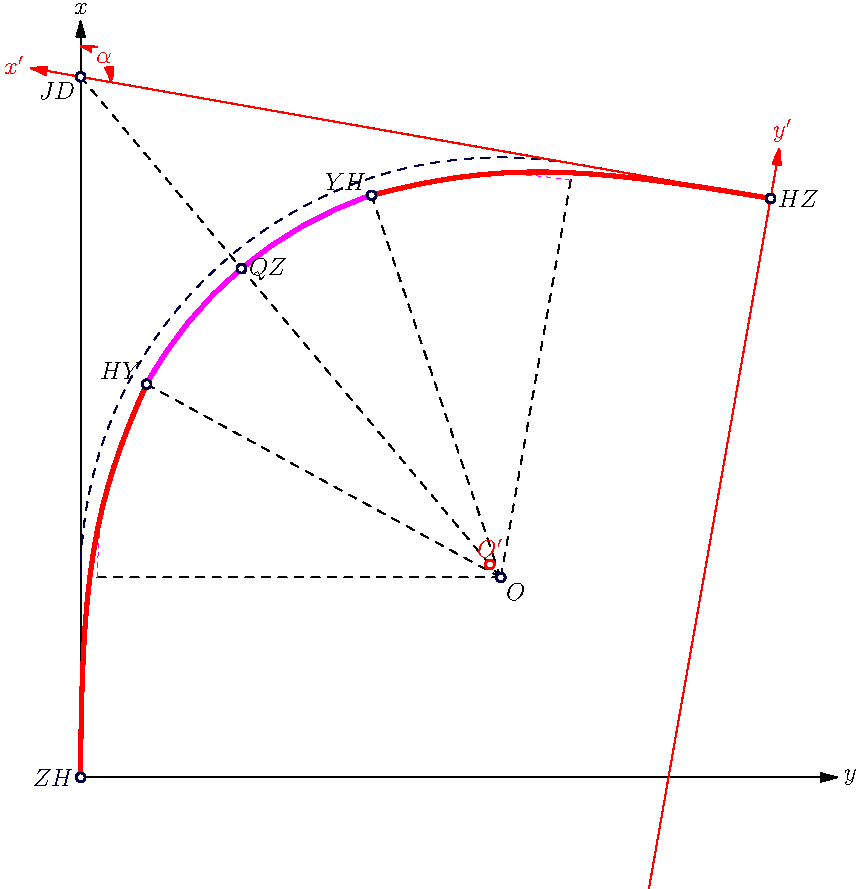
\includegraphics[scale=0.7]{chapter/route/RHY.pdf}
    \caption{缓和曲线的HZ部分坐标计算}
    \label{fig:RHY}
\end{figure}

如图\ref{fig:RHY}所示建立以缓直点HZ为原点,过HZ至JD方向为x轴,
过HZ点的缓和曲线切线为y轴的直角坐标系,计算另一半曲线任意一点的坐标$(x'_i, y'_i)$。
然后,将坐标转换为以ZH点为原点的直角坐标系中。

缓和曲线在HZ坐标系中的坐标可以继续使用公式 \ref{eq:routeZHXY} 计算,然后由图\ref{fig:RHY}
可知将其转换为HZ坐标系中的坐标计算公式为:

\begin{equation}
\left . \begin{aligned}
x'_i &= x_i  \\
y'_i &= - y_i
\end{aligned} \right \}
\label{eq:routeHZPtXY}
\end{equation}

请注意在使用公式 \ref{eq:routeZHXY} 时应将$l_i$替换为 $L-l_i$。

为了将HZ坐标系中的点坐标转换到ZH坐标系中,我们引用公式\ref{eq:routexytoxy}来计算,
请注意公式\ref{eq:routexytoxy}中的$\alpha$为$x'$轴的方位角(即x轴到$x'$轴的水平夹角),
因此图\ref{fig:RHY}应用到公式\ref{eq:routexytoxy}中的$\alpha$ 应为$\alpha + 180 \degree $。
如果将其代入公式\ref{eq:routexytoxy},则有转换公式为:

\begin{equation}
\left . \begin{aligned}
x_i &= x_{HZ} - x'_i  \cos \alpha + y'_i \sin \alpha \\
y_i &= y_{HZ}  -  x'_i \sin \alpha -  y'_i \cos \alpha
\end{aligned} \right \}
\label{eq:routeHZtoZH}
\end{equation}

公式\ref{eq:routeHZtoZH}中的$(x_{HZ}, y_{HZ})$为HZ点在ZH坐标系中的坐标,其值为:

\begin{equation}
\left .
\begin{aligned}
x_{HZ} &= T (1 +  \cos \alpha) \\
y_{HZ} &=  T \sin \alpha
\end{aligned}
\right \}
\label{eq:routeHZXY}
\end{equation}

也可以不用公式\ref{eq:routeHZtoZH},直接将$\alpha+180\degree$代入到
公式\ref{eq:routexytoxy}中进行计算。

在以上计算中,我们以曲线右偏为例的,如果曲线左偏,同样的方法建立坐标系,
x坐标是相同的, y坐标乘以 -1 即可。

\item 曲线上点坐标转换为大地坐标的计算公式为:

由于已经将曲线上的点坐标统一到ZH坐标系中了,我们继续引用公式\ref{eq:routexytoxy}
将ZH切线坐标系坐标转换到大地坐标系(测量坐标系)中,公式中的$\alpha$为$ZH \rightarrow JD$
的坐标方位角。

\end{enumerate}


\subsection{有缓和曲线的圆曲线算例}

缓和曲线的曲率半径$R=1000$,偏转角$\alpha =10.1820$, 右偏,
缓和曲线长$l_0=80$,直缓点ZH的坐标为$(3088256.238, 66798.566)$,
交点JD的坐标为$(3088386.436, 66798.566)$,里程桩号为``K5+5330.198''。
计算出的曲线上各点坐标如表\ref{tab:HYRoute}所示。

\begin{table}[htbp]
\centering
\caption{有缓和曲线的圆曲线计算示例数据表}
\label{tab:HYRoute}
\begin{tabular}{ccccl}
\hline
序号 & 里程	    &        X	   &      Y	   &  备注 \\
\hline
1   & K5+200.000 & 3088256.238 & 66798.566 &  ZH  \\
2   & K5+220.000 & 3088276.238 & 66798.583 &      \\
3   & K5+240.000 & 3088296.238 & 66798.699 &      \\
4   & K5+260.000 & 3088316.235 & 66799.016 &      \\
5   & K5+280.000 & 3088336.225 & 66799.632 &  HY  \\
6   & K5+300.000 & 3088356.200 & 66800.632 &      \\
7   & K5+320.000 & 3088376.150 & 66802.031 &      \\
8   & K5+329.933 & 3088386.048 & 66802.874 &  QZ  \\
9   & K5+339.866 & 3088395.936 & 66803.815 &      \\
10  & K5+359.866 & 3088415.815 & 66806.008 &      \\
11  & K5+379.866 & 3088435.646 & 66808.598 &  YH  \\
12  & K5+399.866 & 3088455.424 & 66811.568 &      \\
13  & K5+419.866 & 3088475.156 & 66814.834 &      \\
14  & K5+439.866 & 3088494.853 & 66818.297 &      \\
15  & K5+459.866 & 3088514.534 & 66821.858 &  HZ  \\
\hline
\end{tabular}

\end{table}

\section{较为完整的线路里程桩计算}

以上曲线要素的计算是按曲线类型单独进行分析编写的,实际上一条线路
是由无数段直线、圆曲线与缓和曲线组成。


                           %%线路要素计算程序设计

\end{document}
